\newif\ifanon\anontrue    % set true to suppress names, etc.
\newif\iffull\fullfalse   % set true for long version

\documentclass[numbers]{sigplanconf}
\listfiles

% The following \documentclass options may be useful:

% preprint      Remove this option only once the paper is in final form.
% 10pt          To set in 10-point type instead of 9-point.
% 11pt          To set in 11-point type instead of 9-point.
% authoryear    To obtain author/year citation style instead of numeric.

\usepackage{amsmath}
\usepackage[table]{xcolor}
\usepackage{mathtools}
\usepackage{bussproofs}
\usepackage{amsthm}
\usepackage{csvsimple}
\usepackage{thmtools,thm-restate}
\usepackage{changepage}
\usepackage{booktabs}
\usepackage{amssymb}
\usepackage{enumitem}
\usepackage{multirow,bigdelim}
\usepackage{siunitx}
\usepackage{listings}
\usepackage{sansmath}
\usepackage{url}
\usepackage{flushend}
\usepackage{microtype}
\usepackage[utf8]{inputenc}
\usepackage{mathpartir}
\usepackage{empheq}
\usepackage{array}
\usepackage{pgfplots}
\usepackage{stmaryrd}
\usepackage{courier}
\usepackage{qtree}
\usepackage[normalem]{ulem}
\usepackage{relsize}
\usepackage{tikz}

\usetikzlibrary{matrix}

%%%% Hyperlinks – must come late!
\usepackage[pdftex,%
            pdfpagelabels,%
            linkcolor=blue,%
            citecolor=blue,%
            filecolor=blue,%
            urlcolor=blue]
           {hyperref}

\newcommand{\Regex}{\ensuremath{r}}         % Regular Expression
\newcommand{\UserDefined}{\ensuremath{U}}   % User Defined
\newcommand{\ExampledRegex}{\ensuremath{er}} % Exampled Regex
\newcommand{\Atom}{\ensuremath{a}}          % Atoms
\newcommand{\Clause}{\ensuremath{cl}}       % Clauses
\newcommand{\DNFRegex}{\ensuremath{dr}}         % Regular Expression
\newcommand{\Context}{\ensuremath{\Gamma}}  % Context
\newcommand{\TypeContext}{\ensuremath{\Delta}} %TypeContext
\newcommand{\String}{\ensuremath{s}}        % String
\newcommand{\ExampleNumberList}{\ensuremath{enl}} %Example Number List
\newcommand{\ExampleNumberListList}{\ensuremath{enll}}
\newcommand{\ExampleStringList}{\ensuremath{esl}}
\newcommand{\StringList}{\ensuremath{sl}}
\newcommand{\Natural}{\ensuremath{n}}
\newcommand{\Interleaving}[1]{\ensuremath{interleaving(#1)}}
\newcommand{\Interleave}{\ensuremath{interleave}}
\newcommand{\BinaryInterleave}[2]{\ensuremath{interleave(#1,#2)}}
\newcommand{\NAryInterleave}[2]{\ensuremath{interleave(#1,\ldots,#2)}}
\newcommand{\Combine}{\ensuremath{combine}}
\newcommand{\List}{\ensuremath{l}}
\newcommand{\ValidCombine}[2]{\ensuremath{validcombine(#1,#2)}}
\newcommand{\Parent}[1]{\ensuremath{parent(#1)}}
\newcommand{\Parented}[1]{\ensuremath{parented(#1)}}
\newcommand{\CombineString}[1]{\ensuremath{combine_{\ExampleStringList}(#1)}}
\newcommand{\CombineList}[1]{\ensuremath{combine_{\ExampleNumberListList}(#1)}}
\newcommand{\Length}[1]{\ensuremath{len(#1)}}


\newcommand{\Lens}{\ensuremath{l}}
\newcommand{\AtomLens}{\ensuremath{al}}
\newcommand{\ClauseLens}{\ensuremath{cll}}
\newcommand{\DNFLens}{\ensuremath{dl}}


\newcommand{\Star}[1]{\ensuremath{#1^*}}
\newcommand{\ConcatLens}[2]{\ensuremath{concat(#1,#2)}}
\newcommand{\SwapLens}[2]{\ensuremath{swap(#1,#2)}}
\newcommand{\OrLens}[2]{\ensuremath{or(#1,#2)}}
\newcommand{\IdentityLens}{\ensuremath{identity}}
\newcommand{\IterateLens}[1]{\ensuremath{iterate(#1)}}
\newcommand{\ComposeLens}[2]{\ensuremath{#1 \circ #2}}

% GRAMMAR OPERATORS
\newcommand{\GBar}{\ensuremath{~|~}}
\newcommand{\GIndent}{\hspace{.5in}}
\newcommand{\GEq}{\ensuremath{::=~}}  
\newcommand{\GEmp}{\ensuremath{\cdot}}



\clubpenalty = 10000
\widowpenalty = 10000
\displaywidowpenalty = 10000

%\setlength{\belowcaptionskip}{-5pt}
%\setlength{\textfloatsep}{15pt}

% Creates a display mode for code in sans serif font
\lstnewenvironment{sflisting}[1][]
  {\lstset{%
    mathescape,
    basicstyle=\small\sffamily,
    aboveskip=5pt,
    belowskip=5pt,
    columns=flexible,
    frame=,
    xleftmargin=1em,#1}\sansmath}
  {}
% end

% Macros
\newcommand{\NameOf}[1]{\texttt{#1}}

\begin{document}

\special{papersize=8.5in,11in}
\setlength{\pdfpageheight}{\paperheight}
\setlength{\pdfpagewidth}{\paperwidth}
\toappear{}

\conferenceinfo{POPL '16}{January 20--22, 2016, St. Petersburg, FL, USA} 
\copyrightyear{2016} 
\copyrightdata{978-1-nnnn-nnnn-n/yy/mm} 

% Uncomment one of the following two, if you are not going for the 
% traditional copyright transfer agreement.

%\exclusivelicense                % ACM gets exclusive license to publish, 
                                  % you retain copyright

%\permissiontopublish             % ACM gets nonexclusive license to publish
                                  % (paid open-access papers, 
                                  % short abstracts)

\titlebanner{DRAFT---do not distribute}        % These are ignored unless
\preprintfooter{to appear in POPL '16}   % 'preprint' option specified.

\title{Synthesizing Bijective Lenses
\ifanon\vspace*{-2cm}\fi
}

\ifanon
\authorinfo{}
           {}
           {}
\maketitle
% \vspace*{-6cm}
\else
\authorinfo{Anders Miltner}
           {Princeton University, USA}
           {}
%            {amiltner@cs.princeton.edu}
\authorinfo{Kathleen Fisher}
           {Tufts University, USA}
           {}
%            {kfisher@eecs.tufts.edu}
\authorinfo{Benjamin Pierce}
           {University of Pennsylvania, USA}
%            {bcpierce@cis.upenn.edu}
           {}
\authorinfo{David Walker}
           {Princeton University, USA}
           {}
%            {dpw@cs.princeton.edu}
\authorinfo{Steve Zdancewic}
           {University of Pennsylvania, USA}
           {}
%            {stevez@cis.upenn.edu}
\maketitle
\fi



\begin{abstract}
  % begin abstract
  \afm{TODO: make sure all adjacent math expressions are separated by more than just
    punctuation, unless they are very short and very regular}
  \afm{TODO: subject verb agreement}
  \emph{Lenses} are a bi-directional technique for specifying conversions between
  data formats.  Specifically, a bijective lens is a declarative program that
  simultaneously specifies a function to convert data from type $A$ to
  type $B$ and a second function to convert data from type $B$ to type
  $A$.  Such programs provide invertibility guarantees, avoiding
  pernicious bugs that can corrupt data and downstream processing.
  Unfortunately, lenses can be quite difficult to write, as the restrictive
  typing which provides guarantees about the program's invertibility also
  heavily restricts what programs are allowed.  To overcome
  this difficulty, we develop an algorithm to automatically synthesize
  bijective lenses from their regular expression types, and
  a small number of examples.  This will allow average programmers to get the
  benefit of lenses' invertibility guarantees, without requiring them to
  understand their complicated type system.

  The rich structure of regular expressions
  makes lens synthesis more complicated than previous work on other
  forms of type-directed synthesis.  Specifically, finding a term to
  bi-directionally map between regular expressions $A$ and $B$ requires
  first finding equivalent regular expressions $A'$ and $B'$ that are
  more algorithmically tractable.
  We show how to manage this search by defining a new language of
  lenses governed by semi-canonical regular expression types and prove it
  sound with respect to a standard language of bijective lenses.  
  We then show
  how to search the reduced space for well-typed lenses that are consistent
  with the given examples.  We demonstrate the effectiveness of our algorithm
  by experimenting on a benchmark suite containing 42 examples
  comprising microbenchmarks, Flash Fill
  examples, and Augeas transformations of Linux configuration files.
  We show we are able to infer lenses for all examples in the
  benchmark suite in an average of 0.134 seconds \afm{TODO: automatically calculate this from CSV}. 
  % end abstract
\end{abstract}

% \category{D.3.1}
% {Programming Languages}
% {Formal Definitions and Theory}
% [Semantics]
\ifanon\else
\category{F.4.1}
{Mathematical Logic and Formal Languages}
{Mathematical Logic}
[Proof Theory]
\category{I.2.2}
{Artificial Intelligence}
{Automatic Pro\-gramming}
[Program Synthesis]

\terms Languages, Theory

\keywords Functional Programming, Proof Search, Program Synthesis, Type Theory
\fi

% begin introduction
\section{Introduction}

The growing dependence on big data makes tools for reliably parsing,
printing, cleaning, and transforming data increasingly important.
One such class of tools is the class of \emph{lenses}~\cite{Focal2005-long},
bi-directional programs that help users solve the classic ``view update problem.''
More specifically, a lens provides a user with two functions, a
\emph{get} function and a \emph{put} function.  The \emph{get}
function translates native data into a new format, or \emph{view}, for
the user.  If the user updates the new view, the corresponding
\emph{put} function can translate the edited data back into
the native format.

Converting data back and forth between representations is a common problem.
This problem arises in serializers and deserializers, models and views, picklers
and unpicklers, and more.
Bidirectional programs express both transformations in a single program, instead
of requiring a program for each transformation.
Bidirectional programming has begun to be used in practice for expressing some
classes of back and forth transformations.
Augeas~\cite{?}, a configuration editing system for linux, uses lens combinators
to provide editable views of configuration files.
The language biXid~\cite{bixid} is developed for expressing bidirectional XML
transformations.
XSugar~\cite{xsugar} is used to convert bidirectionally between XML and non-XML data,
and is used to convert between EpiDoc~\cite{epidoc} and
Leiden+~\cite{leidenplus} formats for
encoding ancient documents~\cite{epidocleidenplus}.

Lenses are popular because they typically come with strong guarantees
about the round-trip behavior.  Such guarantees
help users guard against data corruption while reading and editing
high-value data sources.  These guarantees are often achieved through
the use of domain-specific languages with strong type systems that
guarantee invertability of lens programs~\cite{Focal2005-long,boomerang,symmetric-lenses}.  Unfortunately, such
lens languages are currently quite non-standard.  The
process of writing a lens is challenging, as a user must think
about data conversion in two directions at once --- an
unusual task for the everyday programmer.  As a consequence, 
for the casual user of lenses, learning the language, its type system and its
unorthodox programming style is time-consuming and, in the end,
a disincentive to adopting the technology, despite its advantages.

In order to overcome the difficulty involved in programming
with lenses, we have developed a new system for synthesis of lenses
from their types and a collection of representative examples.  More
specifically, we focus on algorithms for the synthesis of bijective
string lenses.  The types for such lenses are regular expressions,
which describe the format of the source and target strings.  Given
such types, and a very small number of representative examples (sometimes
no examples at all), we synthesize a well-typed lens that implements
a bijection between data formats.

Recently, researchers have developed a number of new algorithms for
synthesis~\cite{yag+:pldi16,osera+:pldi15,frankle+:popl16,armando+:pldi16}.
Many of those
algorithms~\cite{osera+:pldi15,frankle+:popl16,armando+:pldi16} are
directed in part by the syntax of types.  For instance, to find an
expression with type $A \rightarrow B$, such algorithms will assume
that the expression in question is a function with the form $\lambda
x{:}A. e$, and they will continue the search for an expression $e$
with type $B$ under the hypothesis that the parameter $x$ has type
$A$.  In the case of the simply typed lambda calculus, such an
approach reduces the complexity of the search for terms inhabiting the
type without losing completeness.  Lenses are defined by a richer type system
than the simply typed lambda calculus,
with their regular expression types, as
there are many equivalent ways to express the same regular expression.
Unfortunately, this makes simple
syntax-directed algorithms not directly applicable.

In order to explain the major components of our synthesis algorithm,
we will consider a running example involving conversion between citations given
in (highly simplified) BibTex and EndNote formats.  Our BibTex format
consists entirely of specifying a list of authors on a single line as follows.
\begin{lstlisting}
author={Conway, John and Kleene, Stephen Cole}
\end{lstlisting}
Our EndNote format contains the same information, but uses different separators,
rearranges the order of first and last names, and uses a separate line for each
author. 
\begin{lstlisting}
% A John Conway
% A Stephen Cole Kleene
\end{lstlisting}

\begin{figure}
\begin{lstlisting}
Name = [A-Z][a-z]*
Names = (" " Name)*

BNames = Name ", " Name Names
Bib = ""
    | "author={" BNames (" and " BNames)* "},"

ENames = Name Names " " Name
End = ("%A " ENames "\n")*

BibEnd : Bib <=> End = {
"author={Conway, John and Kleene, Stephen Cole}"
<-> "%A John Conway\n%A Stephen Cole Kleene" }
\end{lstlisting}
  \caption{Synthesis Problem Definition: Idealized Bibtex to EndNote}
  \label{fig:bibend-spec}
\end{figure}

Figure~\ref{fig:bibend-spec} presents
the user's specification of such a problem.  In general, such specifications are
given by defining the source and target data formats~\footnote{Lenses
  operate both left-to-right and right-to-left, so both formats are sometimes
  sources and sometimes targets. Nevertheless, we will often call the
  format on the left, the ``source,'' and the format on the right, 
  the ``target.''} as well as some examples.  In this case, the lens
we wish to synthesize is \CF{BibEnd}.  It converts between 
the formats \CF{Bib} and \CF{End}.
Such formats are defined using a standard syntax for regular expressions.
Intermediate regular expressions are named in order to facilitate
construction of complex formats.


\paragraph*{The Central Challenge.}
To illustrate the central challenge facing the design of our synthesis system
in greater detail,
consider the concatenation lens, $\ConcatLensOf{\Lens_1}{\Lens_2}$,
one of the simplest string lens combinators.  
When viewed from left to right, this lens defines a function \emph{get}, which,
given a string 
$\String$, divides $\String$ into two substrings $\String_1$ 
and $\String_2$, applies $\Lens_1$ to the first, yielding $t_1$,
and $\Lens_2$ to the second, yielding $t_2$.  When viewed from
right to left, it defines a second function \emph{put}, which maps
data back from strings $t$ to strings $s$ in an analogous way.

The type system for lenses ensures such \emph{get} and \emph{put} functions
satisfy strong invertibility properties.  In our case, the two functions
form a bijection.  In general, to 
describe the type of a lens, we write $\Lens \OfType \Regex \Leftrightarrow
\RegexAlt$, which may be read ``lens $\Lens$ converts back and forth between
data in the language of regular expression $\Regex$ and data in the language
of regular expression $\RegexAlt$''.  More specifically, to give a type
to the concatenation lens, we use the following typing rule.
\[
  \inferrule
  {
    \Lens_1 \OfType \Regex_1 \Leftrightarrow \RegexAlt_1\\
    \Lens_2 \OfType \Regex_2 \Leftrightarrow \RegexAlt_2\\\\
    \UnambigConcatOf{\Regex_1}{\Regex_2}\\
    \UnambigConcatOf{\RegexAlt_1}{\RegexAlt_2}
  }
  {
    \ConcatLensOf{\Lens_1}{\Lens_2} \OfType \Regex_1\Regex_2 \Leftrightarrow \RegexAlt_1\RegexAlt_2
  }
\]
Above, the notation $\UnambigConcatOf{\Regex_1}{\Regex_2}$ asserts that $\Regex_1$ and $\Regex_2$ are
unambiguously concatenable, meaning there is
exactly one way to divide up any
string $\String$ in the language of $\Regex_1\Regex_2$ into $\String_1$
and $\String_2$ such that $\String_1$ is in the language of $\Regex_1$
and $\String_2$ is in the language of $\Regex_2$.  These unambiguous
concatenation constraints guarantee the \emph{get} and \emph{put}
functions are indeed functions and that they form a bijection if
the underlying lenses are bijective.

Now, with these typing rules in hand, consider trying to search for
a lens with the type $(A B) C \Leftrightarrow A' (B' C')$ where
we know of lenses with types 
$A \Leftrightarrow A'$, $B \Leftrightarrow B'$, and 
$C \Leftrightarrow C'$.  A straightforward,
syntax-directed search suggests applying the rule for concatenation,
and looking for two simpler lenses with the types $A B \Leftrightarrow A'$
and $C \Leftrightarrow B' C'$ respectively.  Unfortunately, at this point,
we are simply stuck---we have no lenses with those types.  Of course,
the natural
solution to this problem
is to introduce a type conversion rule to the system:
\[
  \inferrule
  {
    \Lens \OfType \Regex_1 \Leftrightarrow \Regex_2\\
    \Regex_1 \equiv \Regex_1'\\
    \Regex_2 \equiv \Regex_2'
  }
  {
    \Lens \OfType \Regex_1' \Leftrightarrow \Regex_2'
  }
\]
With such a type conversion rule, we could first 
convert the type $(A B) C \Leftrightarrow A' (B' C')$
to the better aligned $(A B) C \Leftrightarrow (A' B') C'$.
When we then proceed with structure decomposition using the
concatenation rule, we generate sub-problems involving
finding lenses for types
$A \Leftrightarrow A'$, $B \Leftrightarrow B'$, and 
$C \Leftrightarrow C'$, which is just what we had in hand.

Because equivalence of regular expressions is decideable, when
given a lens $\Lens$ with type $\Regex_1 \Leftrightarrow \Regex_2$,
it is easy to \emph{check} whether that lens also has type 
$\Regex_1' \Leftrightarrow \Regex_2'$, and lens programming languages
such as Boomerang \cite{foster:thesis} do so.  However, 
when we turn to synthesis and are given the lens type 
$\Regex_1' \Leftrightarrow \Regex_2'$ and the option to apply this
rule, the search space becomes unmanageably large --- we must guess
some arbitrary new regular expressions $\Regex_1$ and $\Regex_2$ that are
equivalent to  $\Regex_1'$ and $\Regex_2'$ respectively
and there are infinitely many such regular expressions to choose
from.

Furthermore, removing the composition operator from Boomerang reduces
expressivity.
That means to have a synthesis procedure that can synthesize all lenses,
composition lenses must be synthesized.
To synthesize a composition lens between $\Regex_1$ and $\Regex_2$, an arbitrary
$\Regex_3$ must be found,
and then two lenses of types $\Regex_1 \Leftrightarrow \Regex_3$ and
$\Regex_3 \Leftrightarrow \Regex_2$ must also be created.  Searching through all
possible
regular expressions for the correct $\Regex_3$ becomes a difficult infinite search
problem.

In essence, to naively apply type-directed synthesis techniques would involve
solving the problem of search \emph{in three dimensions}:  In one
dimension, we must search for a regular expression \emph{type}
with an appropriate ``syntactic shape''.  In a second dimension,
we must search for a lens \emph{expression} that has the given type and
is consistent with the user's examples.  In a final dimension, we must search
for intermediary regular expressions for composing lenses.

\paragraph*{Our Solution.}  Our solution to this problem is to define
a new language of lenses that
cuts down the synthesis search space \emph{in all dimensions}.
This language is designed so that its regular expression types are limited 
to those in a normalized form.  This normalized form
demands that regular expressions be defined as a flattened 
union of concatenated strings and atoms, where each atom is a user defined data
type or the Kleene star of an expression that is recursively in normal form.
When converted into this normalized form, two regular expressions that 
differed only by associativity of concatenation will be syntactically equal.
For example, rather than searching for a lens with type 
$(A B) C \Leftrightarrow A' (B' C')$, our algorithm will always search
for one with type  $(A B) C \Leftrightarrow (A' B') C'$

More generally, many, but not all, structural incongruities that
prevent the existence of lenses disappear.
Not all structural incogruities disappear because our normalized regular expressions
are only \emph{pseudo-canonical}.  For instance, our normal form
does not automatically unify lenses such as
$A B* \Leftrightarrow A (\epsilon + BB*)$ that result from an
unrolling of Kleene Star.
Consequently, we structure our synthesis algorithm in two parts:  The
first is a syntax-directed search for a lens based on the structure of the given
regular expression types and, if that fails, the second is a search,
using a subset of Conway's axioms~\cite{conway} for 
equivalent regular expression types that might allow a new search
in the first phase of the search to succeed.

Furthermore, the specialized lenses between these
pseudo-canonical forms can express more than lenses without composition.
Indeed, despite not having a composition operator, these specialized lenses 
are closed under composition.  This reduces the search space by an entire
dimension!  The synthesis algorithm no longer needs to search through possible
regular expressions for the central type in compositions.

The types
describing data formats may be very large --- they are regular
grammars describing complex data formats.  This is another complication that
arises in this synthesis setting, but not elsewhere in the literature on
type-directed synthesis.  On the one hand, this is
very useful as such types provide a wealth of information that constrains
the search process effectively.  On the other hand, there is a lot of
data that must be managed carefully by the synthesis system.
One important observation is that users naturally construct
such types compositionally\afm{Nicolas felt this was confusing to have this word
  for building out of subcomponents, when a composition operator is also
  discussed.  However, I can't think of a different way to put this, any ideas?},
using named abbreviations for subcomponents.
The structure inherent in these named abbreviations can be 
exploited by the synthesis algorithm to speed up the search dramatically.

For example, if the name $A$ appears once on both the left and the right,
the system will hypothesize that the identity lens can be used to convert
between occurrences of $A$.  On the other hand, if the name $A$ appears
on the left, but not on the right, the system will determine that the
name $A$ should be replaced by its definition.  Likewise, differing
numbers of occurrences of names can serve as a guide for unrolling
Kleene star or applying other regular expression equivalence axioms.
Hence, in general, to guide the transformation of regular expression
types, we define a pseudometric based on the occurrence of names.

\paragraph*{Contributions.}  We have designed and implemented
a new system for the synthesis of bijective string lenses.
In addition, this paper makes the following contributions:

\begin{itemize}
\item It defines a new language of lenses designed specifically for synthesis
  with types based on pseudo-canonical regular expressions, with a term 
  language to match.
\item We formalize the semantics of the language and prove it sound with
  respect to an existing, standard language for bijective string lenses.
\item We designed a type-directed, two-dimensional 
  algorithm for synthesizing lenses in our new domain-specific language.
\item We developed a collection of optimizations that speed up the basic
  synthesis algorithm.
\item We have implemented the language and evaluated it on a range of
  over 40 benchmarks including micro-benchmarks, a few examples from FlashFill,
  and a number of examples from the Augeas system for transforming linux
  file formats.  Our synthesis algorithm succeeds on all of our
  benchmarks, with a synthesis time of typically less than 1 second.
\end{itemize}
% end introduction

% begin background
\section{Background}

\subsubsection{Languages and Alphabets}

A \textit{character}, written \Character{} or \CharacterAlt{}, is a symbol.
An \textit{alphabet}, written \Alphabet{}, is set of characters.
A \textit{string}, written \String{} or \StringAlt{}, is a sequence of characters.
The empty string is written \EmptyString{}.
The set of all strings is written \StarOf{\Alphabet}.
A \textit{language}, written \Language{}, is a subset of \StarOf{\Alphabet}.

If \String{} and \StringAlt{} are strings, with
$\String=\Character_1\ldots\Character_n$,
and $\StringAlt=\CharacterAlt_1\ldots\CharacterAlt_m$,
then the \textit{concatenation} of \String{} and \StringAlt{},
written \String{}\Concat\StringAlt{}, is defined as
$\Character_1\ldots\Character_n\CharacterAlt_1\ldots\CharacterAlt_m$.

If $\Language$ is a language, where
for all $n\in\Nats$ and for all strings
$\String_1,\StringAlt_1,\ldots,\String_n,\StringAlt_n\in\Language$, if
$\String_1\Concat\ldots\Concat\String_n=\StringAlt_1\Concat\ldots\Concat\StringAlt_n$
then $\String_i=\StringAlt_i$ for all $i$,
that language is \textit{unambiguously iterable},
written $\UnambigItOf{\Language}$.


\subsubsection{Regular Expressions}

The syntax for the regular expressions we use is given below.

\begin{tabular}{l@{\hspace*{5mm}}l@{\ }c@{\ }l@{\hspace*{5mm}}>{\itshape\/}l}

  (Strings)& \String{},\StringAlt{} & \GEq{} & $\String\in\StarOf{\Sigma}$ \\
  (Regexs)& \Regex{},\RegexAlt{} & \GEq{} & s & \BaseRegexType{} \\
           & & & \GBar{} $\emptyset$ & \EmptyRegexType{} \\
           & & & \GBar{} \Regex{}* & \StarRegexType{} \\
           & & & \GBar{} $\RegexConcat{\Regex_1}{\Regex_2}$ & \ConcatRegexType{} \\
           & & & \GBar{} $\RegexOr{\Regex_1}{\Regex_2}$ & \OrRegexType{} \\
\end{tabular}

\afm{$\Regex_1 \Concat \Regex_2$ was $\Regex_1 \Regex_2$ before, what is the correct one?}

$\Regex^n$ can be used for shorthand for $n$ instances of $\Regex$ concatenated
with each other.
$\Regex^{<n}$ can be used for shorthand for $\Regex^0 \Or \Regex^1 \Or \ldots
\Or \Regex^{n-1}$.
These regular expressions have an underlying semantics to express languages,
formalized below
\[
  \begin{array}{lcl}
    \LanguageOf{\String} &=& \{\String\}\\
    \LanguageOf{\emptyset} &=& \{\}\\
    \LanguageOf{\RegexConcat{\Regex_1}{\Regex_2}} &=&
                                                      \{\StringConcat{\String_1}{\String_2} \SuchThat
                                                      \String_1\in\LanguageOf{\Regex_1} \BooleanAnd \String_2\in\LanguageOf{\Regex_2}\}\\
    \LanguageOf{\RegexOr{\Regex_1}{\Regex_2}} &=&
                                                  \{\String \SuchThat
                                                  \String\in\LanguageOf{\Regex_1} \BooleanOr \String\in\LanguageOf{\Regex_2}\}\\
    \LanguageOf{\StarOf{\Regex}} &=&
                                     \{\String_1\Concat\ldots\Concat\String_n \SuchThat
                                     n\in\Nats \wedge \String_i\in\LanguageOf{\Regex}\}
  \end{array}
\]

Two regular expressions, $\Regex$, $\RegexAlt$ are said to be 
\textit{unambiguously concatenable}, written
$\Regex\UnambigConcat\RegexAlt$ if, 
for all strings $\String_1,\StringAlt_1\in\LanguageOf{\Regex}$ and
$\String_2,\StringAlt_2\in\LanguageOf{\RegexAlt}$,
$\String_1\Concat\String_2=\StringAlt_1\Concat\StringAlt_2$ implies
$\String_1=\StringAlt_1$ and $\String_2=\StringAlt_2$.

If $\Regex$ is a regular expression, where $\UnambigItOf{\LanguageOf{\Regex}}$,
then that regular expression is \textit{unambiguously iterable},
written $\UnambigItOf{\Regex}$.

A regular expression $\Regex$ is \textit{strongly unambiguous} if $\Regex =
\String$, $\Regex = \emptyset$, or the following conditions are held:
\begin{enumerate}
\item If $\Regex = \Regex_1 \Concat \Regex_2$ then $\Regex_1 \UnambigConcat
  \Regex_2$, and $\Regex_1$ and $\Regex_2$ are strongly unambiguous
\item If $\Regex = \Regex_1 \Or \Regex_2$ then $\Regex_1 \Intersect \Regex_2 =
  \emptyset$, and $\Regex_1$ and $\Regex_2$ are strongly unambiguous
\item If $\Regex = \StarOf{(\Regex')}$, then $\UnambigItOf{(\Regex')}$ and
  $\Regex'$ is strongly unambiguous
\end{enumerate}


% fig:regex-equivalence-rules
\begin{figure}
  \centering
  \begin{tabular}{@{}r@{\hspace{1em}}c@{\hspace{1em}}l@{}r@{}}
    \Regex{} & $\equiv$ & \Regex{} & \EqualityRule{}  \\
    \RegexOr{\Regex}{\emptyset} & $\equiv$ & \Regex{} & \OrIdentityRule{} \\
    $\RegexConcat{\Regex}{\emptyset}$ & $\equiv$ & $\emptyset$ & \EmptyProjectionRuleRightRule{} \\
    $\RegexConcat{\emptyset}{\Regex}$ & $\equiv$ & $\emptyset$ & \EmptyProjectionRuleLeftRule{} \\
    \RegexConcat{(\RegexConcat{\Regex{}}{\Regex'})}{\Regex''} & $\equiv$ & \RegexConcat{\Regex{}}{(\RegexConcat{\Regex'}{\Regex''})} & \ConcatAssocRule{}  \\
    \RegexOr{(\RegexOr{\Regex}{\Regex'})}{\Regex''} & $\equiv$ & \RegexOr{\Regex}{(\RegexOr{\Regex'}{\Regex''})} & \OrAssociativityRule{}  \\
    \RegexOr{\Regex{}}{\RegexAlt{}} & $\equiv$ & \RegexOr{\RegexAlt{}}{\Regex{}} & \OrCommutativityRule{}\\
    \RegexConcat{\Regex{}}{(\RegexOr{\Regex{}'}{\Regex{}''})} & $\equiv$ & \RegexOr{(\RegexConcat{\Regex{}}{\Regex{}'})}{(\RegexConcat{\Regex{}}{\Regex{}''})} & \DistributivityLeftRule{} \\
    \RegexConcat{(\RegexOr{\Regex{}'}{\Regex{}''})}{\Regex{}} & $\equiv$ & \RegexOr{(\RegexConcat{\Regex{}'}{\Regex{}})}{(\RegexConcat{\Regex{}''}{\Regex{}})} & \DistributivityRightRule{} \\
    \RegexConcat{\Regex{}}{\EmptyString{}} & $\equiv$ & \Regex{} & \ConcatIdentityRule{} \\
    \StarOf{(\RegexOr{\Regex{}}{\RegexAlt{}})} & $\equiv$ & \RegexConcat{\StarOf{(\RegexConcat{\StarOf{\Regex{}}}{\RegexAlt{}})}}{\StarOf{\Regex{}}} & \SumstarRule{}\\
    \StarOf{(\RegexConcat{\Regex{}}{\RegexAlt{}})} & $\equiv$ & \RegexOr{\EmptyString{}}{(\RegexConcat{\RegexConcat{\Regex{}}{\StarOf{(\RegexConcat{\RegexAlt{}}{\Regex{}})}}}{\RegexAlt{}})} & \ProductstarRule{} \\
    ${(\Regex{}^*)}^*$ & $\equiv$ & \StarOf{\Regex{}} & \StarstarRule{} \\
    \StarOf{(\RegexOr{\Regex}{\RegexAlt})} & $\equiv$ & $\StarOf{(\RegexConcat{(\RegexOr{\Regex}{\RegexAlt})}{\RegexOr{\RegexAlt}{\RegexConcat{{(\RegexConcat{\Regex}{\StarOf{\RegexAlt}})}^n}{\Regex}}})}\Concat$ & \DicyclicityRule{}\\
             & & $(\EmptyString\Or(\RegexOr{\Regex}{\RegexAlt})\Concat$\\
             & & $({(\RegexConcat{\Regex}{\StarOf{\RegexAlt}})}^0\Or\ldots\Or{(\RegexConcat{\Regex}{\StarOf{\RegexAlt}})}^n))$
  \end{tabular}
  \caption{Regular Expression Equivalences}
  \label{fig:regex-equivalence-rules}
\end{figure}

% fig:definitional-equivalence-rules
\begin{figure}
  \centering
  \begin{tabular}{@{}r@{\hspace{1em}}c@{\hspace{1em}}l@{}r@{}}
    \Regex{} & $\DefinitionalEquiv$ & \Regex{} & \EqualityRule{}  \\
    \RegexOr{\Regex}{\emptyset} & $\DefinitionalEquiv$ & \Regex{} & \OrIdentityRule{} \\
    $\RegexConcat{\Regex}{\emptyset}$ & $\DefinitionalEquiv$ & $\emptyset$ & \EmptyProjectionRuleRightRule{} \\
    $\RegexConcat{\emptyset}{\Regex}$ & $\DefinitionalEquiv$ & $\emptyset$ & \EmptyProjectionRuleLeftRule{} \\
    \RegexConcat{(\RegexConcat{\Regex{}}{\Regex'})}{\Regex''} & $\DefinitionalEquiv$ & \RegexConcat{\Regex{}}{(\RegexConcat{\Regex'}{\Regex''})} & \ConcatAssocRule{}  \\
    \RegexOr{(\RegexOr{\Regex}{\Regex'})}{\Regex''} & $\DefinitionalEquiv$ & \RegexOr{\Regex}{(\RegexOr{\Regex'}{\Regex''})} & \OrAssociativityRule{}  \\
    \RegexOr{\Regex{}}{\RegexAlt{}} & $\DefinitionalEquiv$ & \RegexOr{\RegexAlt{}}{\Regex{}} & \OrCommutativityRule{}\\
    \RegexConcat{\Regex{}}{(\RegexOr{\Regex{}'}{\Regex{}''})} & $\DefinitionalEquiv$ & \RegexOr{(\RegexConcat{\Regex{}}{\Regex{}'})}{(\RegexConcat{\Regex{}}{\Regex{}''})} & \DistributivityLeftRule{} \\
    \RegexConcat{(\RegexOr{\Regex{}'}{\Regex{}''})}{\Regex{}} & $\DefinitionalEquiv$ & \RegexOr{(\RegexConcat{\Regex{}'}{\Regex{}})}{(\RegexConcat{\Regex{}''}{\Regex{}})} & \DistributivityRightRule{} \\
    \RegexConcat{\Regex{}}{\EmptyString{}} & $\DefinitionalEquiv$ & \Regex{} & \ConcatIdentityRule{} \\
    \StarOf{\Regex{}} & $\DefinitionalEquiv$ & \RegexOr{\EmptyString{}}{(\RegexConcat{\Regex{}}{\StarOf{{\Regex{}}}})} & \UnrollstarRule{} \\
    \StarOf{\Regex{}} & $\DefinitionalEquiv$ & \RegexConcat{\Regex^{<n}}{\StarOf{(\Regex^n)}} & \QuotientstarRule{}
  \end{tabular}
  \caption{Definitional Regular Expression Equivalences}
  \label{fig:definitional-equivalence-rules}
\end{figure}

\section{Regular Expression Equivalences}

If $\Regex$ and $\RegexAlt$ are regular expressions, where
$\LanguageOf{\Regex}=\LanguageOf{\RegexAlt}$, those two regular expressions
are called \textit{equivalent}, written $\Regex\equiv\RegexAlt$.
There exists an equational theory for determining if two regular expressions
are equivalent, presented by Conway \cite{conway}, and proven complete by Krob
\cite{Krob}, shown in Figure~\ref{fig:regex-equivalence-rules}.  This equational
theory consists of the semiring axioms, and a number of axioms dealing with the
equivalences on $^*$.  \ProductstarRule{} is an axiom corresponding to separating the
zero case from the one or greater case in stars.  \SumstarRule{} takes an iteration of two
different regular expressions, and groups together when one regular expression occurs,
separated by when the other regular expression occurs.  \StarstarRule{} is used
to 
introduce ambiguity.  \DicyclicityRule{} is used to separate out the iteration
of two elements into a quotiented portion, and a remainder portion.  An
equational theory provides a straightforward search procedure for generating
equivalent regular expressions.

It is possible to look into other equivalence rules than this.  In particular,
we are interested in equivalence rules that are \emph{finer} than those in
Figure~\ref{fig:regex-equivalence-rules}, to maintain the invariant that
equivalent regular expressions have the same language.
Our algorithm is based on a rewriting system, and it is necessary for that
rewriting system to be confluent, to reduce the need for an analogue to
\ComposeLensRule{}.  Furthermore, for the same reason, if two regular
expressions have a lens between them, any rewrite rule on one side must be able
to be
mimicked on the other.  As such, we need equivalence rules that can be written
as the transitive, reflexive, and symmetric closure of a rewrite relation that
satisfies the requirement of our algorithm.

A subset of
the regular expression equivalence rules, the \textit{definitional equivalence
  rules} are shown in
Figure~\ref{fig:definitional-equivalence-rules}.  These equivalence rules are
unable to express all of the equivalences of language equivalence.  In this
subset, the full generality of \SumstarRule{} is not present, the full
generality of \DicyclicityRule{} is not present, \StarstarRule{} is not present,
and \SumstarRule{} is not present.  \StarstarRule{} is a rule that introduces
ambiguity, so removing it no longer allows ambiguity to be introduced.
  The
removal of \SumstarRule{} no longer allows for different choices of an
interation to be grouped by when they occur.  \ProductstarRule{} is similar to
\UnrollstarRule{}, though more expressible.
\ProductstarRule{}
allows for the order of what's under the star to be changed, by popping
different parts of the regular expression out on different sides of the star.
\DicyclicityRule{} is
similar to \QuotientstarRule{}, in that it breaks a repetition of a regular
expression into different parts based on it's divisibility by a number $n$.  However
it also takes into account different parts of the regular expression repeating.

The primary difference between the regular expression equivalence rules and the
definitional equivalence rules, are that the regular expression equivalence
rules allow for breaking up parts of the regular expression under a star by
grouping together different parts of the repetition, whereas the definitional
equivalence rules breaks parts of a regular expression under a star up only by
how many times the already defined repetition occurs.

This was the largest subset of the Regular Expression equivalence rules we could
find that still satisfied the required properties.  There may be larger ones,
but this one was able to handle the equivalences that showed up in practice.

\section{Bijective Lenses}

% fig:lens-syntax
\begin{figure}
  \centering
  \begin{tabular}{l@{\ }l@{\ }c@{\ }l@{\ }>{\itshape\/}r}
    % REGEX
    (Lenses)& \Lens{} & \GEq{} & $\ConstLensOf{s_1 \in \StarOf{\Alphabet}}{s_2 \in \StarOf{\Alphabet}}$ & Const \\
            & & & \GBar{} $\IterateLensOf{\Lens}$ & Iterate \\
            & & & \GBar{} $\ConcatLensOf{\Lens_1}{\Lens_2}$ & Concat \\
            & & & \GBar{} $\SwapLensOf{\Lens_1}{\Lens_2}$ & Swap\\
            & & & \GBar{} $\OrLensOf{\Lens_1}{\Lens_2}$ & Or\\
            & & & \GBar{} $\ComposeLensOf{\Lens_1}{\Lens_2}$ & Compose\\
            & & & \GBar{} $\IdentityLensOf{\Regex}$ & Identity
  \end{tabular}
  \caption{Lens Syntax}
  \label{fig:lens-syntax}
\end{figure}

% fig:lens-semantics
\begin{figure}
  \[
    \begin{array}{rcl}
      \SemanticsOf{const(\String_1,\String_2)} &=& \SetOf{(\String_1,\String_2)}\\

      \SemanticsOf{\IterateLensOf{\Lens}} &=& \SetOf{(\String_1\Concat\ldots\Concat\String_n,
                                              \StringAlt_1\Concat\ldots\Concat\StringAlt_n)\SuchThat
                                              (\String_i,\StringAlt_i)\in\SemanticsOf{\Lens}}\\

      \SemanticsOf{\ConcatLensOf{\Lens_1}{\Lens_2}} &=&
                                                        \SetOf{(\String_1\Concat\String_2,\StringAlt_1\Concat\StringAlt_2)\SuchThat\\
                                               & & \hspace*{2em}(\String_1,\StringAlt_1)\in\SemanticsOf{\Lens_1}\BooleanAnd
                                                   (\String_2,\StringAlt_2)\in\SemanticsOf{\Lens_2}}\\

      \SemanticsOf{\SwapLensOf{\Lens_1}{\Lens_2}} &=&
                                                      \SetOf{(\String_1\Concat\String_2,\StringAlt_2\Concat\StringAlt_1)\SuchThat\\
                                               & & \hspace*{2em}(\String_1,\StringAlt_1)\in\SemanticsOf{\Lens_1}\BooleanAnd
                                                   (\String_2,\StringAlt_2)\in\SemanticsOf{\Lens_2}}\\

      \SemanticsOf{\OrLensOf{\Lens_1}{\Lens_2}} &=&
                                                    \SetOf{(\String,\StringAlt)
                                                    \SuchThat(\String,\StringAlt)\in\SemanticsOf{\Lens_1}
                                                    \BooleanOr(\String,\StringAlt)\in\SemanticsOf{\Lens_2}}\\

      \SemanticsOf{\ComposeLensOf{\Lens_1}{\Lens_2}} &=&
                                                         \SetOf{(\String_1,\String_3)\SuchThat\exists\String_2\\
                                               & & \hspace*{2em}(\String_1,\String_2)\in\SemanticsOf{\Lens_1}\BooleanAnd
                                                   (\String_2,\String_3)\in\SemanticsOf{\Lens_2}}\\

      \SemanticsOf{\IdentityLensOf{\Regex}} &=& \SetOf{(\String,\String)
                                                \SuchThat \String\in
                                                \LanguageOf{\Regex}}
    \end{array}
  \]
  \caption{Lens Semantics}
  \label{fig:lens-semantics}
\end{figure}

% fig:lens-semantics
\begin{figure}
  \centering
  \begin{mathpar}
    \inferrule[\ConstantLensRule{}]
    {
      \String_1 \in \StarOf{\Sigma}\\
      \String_2 \in \StarOf{\Sigma}
    }
    {
      \ConstLensOf{\String_1}{\String_2} \OfType \String_1 \Leftrightarrow \String_2
    }

    \inferrule[\IterateLensRule{}]
    {
      \Lens \OfType \Regex \Leftrightarrow \RegexAlt\\
      \UnambigItOf{\Regex}\\
      \UnambigItOf{\RegexAlt}
    }
    {
      \IterateLensOf{\Lens} \OfType \StarOf{\Regex} \Leftrightarrow \StarOf{\RegexAlt}
    }

    \inferrule[\ConcatLensRule{}]
    {
      \Lens_1 \OfType \Regex_1 \Leftrightarrow \RegexAlt_1\\
      \Lens_2 \OfType \Regex_2 \Leftrightarrow \RegexAlt_2\\\\
      \UnambigConcatOf{\Regex_1}{\Regex_2}\\
      \UnambigConcatOf{\RegexAlt_1}{\RegexAlt_2}
    }
    {
      \ConcatLensOf{\Lens_1}{\Lens_2} \OfType \Regex_1\Regex_2 \Leftrightarrow \RegexAlt_1\RegexAlt_2
    }

    \inferrule[\SwapLensRule{}]
    {
      \Lens_1 \OfType \Regex_1 \Leftrightarrow \RegexAlt_1\\
      \Lens_2 \OfType \Regex_2 \Leftrightarrow \RegexAlt_2\\\\
      \UnambigConcatOf{\Regex_1}{\Regex_2}\\
      \UnambigConcatOf{\RegexAlt_2}{\RegexAlt_1}
    }
    {
      \SwapLensOf{\Lens_1}{\Lens_2} \OfType \Regex_1\Regex_2 \Leftrightarrow \RegexAlt_2\RegexAlt_1
    }

    \inferrule[\OrLensRule{}]
    {
      \Lens_1 \OfType \Regex_1 \Leftrightarrow \RegexAlt_1\\
      \Lens_2 \OfType \Regex_2 \Leftrightarrow \RegexAlt_2\\\\
      \UnambigOrOf{\LanguageOf{\Regex_1}}{\LanguageOf{\Regex_2}}\\ \UnambigOrOf{\LanguageOf{\RegexAlt_1}}{\LanguageOf{\RegexAlt_2}}
    }
    {
      \OrLensOf{\Lens_1}{\Lens_2} \OfType \Regex_1 | \RegexAlt_1 \Leftrightarrow \Regex_2 | \RegexAlt_2
    }

    \inferrule[\ComposeLensRule{}]
    {
      \Lens_1 \OfType \Regex_1 \Leftrightarrow \Regex_2\\
      \Lens_2 \OfType \Regex_2 \Leftrightarrow \Regex_3\\
    }
    {
      \ComposeLensOf{\Lens_2}{\Lens_1} \OfType \Regex_1 \Leftrightarrow \Regex_3
    }

    \inferrule[\RewriteRegexLensRule{}]
    {
      \Lens \OfType \Regex_1 \Leftrightarrow \Regex_2\\
      \Regex_1 \DefinitionalEquiv \Regex_1'\\
      \Regex_2 \DefinitionalEquiv \Regex_2'
    }
    {
      \Lens \OfType \Regex_1' \Leftrightarrow \Regex_2'
    }

    \inferrule[\IdentityLensRule{}]
    {
      \Regex \text{ is strongly unambiguous}
    }
    {
      \IdentityLensOf{\Regex} \OfType \Regex \Leftrightarrow \Regex
    }
  \end{mathpar}

  \caption{Lens Typing}
  \label{fig:lens-typing}
\end{figure}

Bijective lenses are a certain class of lenses which define bijective functions
between the languages of regular expressions.
The syntax for these bijective lenses is provided in Figure~\ref{fig:lens-syntax}.
The semantics and for these lenses are defined in
Figure~\ref{fig:lens-semantics}.  If $(\String_1,\String_2) \in
\SemanticsOf{\Lens}$, then $\Lens$ \emph{maps between} $\String_1$ and
$\String_2$.
The typing is given in Figure~\ref{fig:lens-typing}, where a well
typed program provides a bijection between the language of the regular expressions
of its type.

The simplest lens in the combinator language is the the constant lens between
strings $\String$, and $\StringAlt$, $\ConstLensOf{\String}{\StringAlt}$.
The lens $\ConstLensOf{\String_1}{\String_2}$, when operated left-to-right,
replaces the string $\String_1$ with $\String_2$, and when operated
right-to-left, replaces string $\String_2$ with $\String_1$.

Each of the other lenses manipulates structured data.  For instance,
$\ConcatLensOf{\Lens_1}{\Lens_2}$ operates by applying $\Lens_1$ to the left
portion of a string, and $\Lens_2$ to the right, and concatenating the results.
The combinator
$\SwapLensOf{\Lens_1}{\Lens_2}$ does the same as $\ConcatLensOf{\Lens_1}{\Lens_2}$
but it swaps the results before concatenating.
The combinator $\OrLensOf{\Lens_1}{\Lens_2}$ operates by applying either $\Lens_1$ or $\Lens_2$
to the string.  The combinator $\IterateLensOf{\Lens}$ operates by repeatedly
applying $\Lens$ to subparts of a string.  The combinator
$\ComposeLensOf{\Lens_1}{\Lens_2}$ operates by applying $\Lens_1$ then $\Lens_2$
when operating left to right, and applying $\Lens_2$ then $\Lens_1$ when
operating right to left.
$\IdentityLensOf{\Regex}$ operates by applying the identity transformation to
any string in $\LanguageOf{\Regex}$.
% end background

% begin extended-example
\section{Lens Synthesis by Example}

Recall the previous example of synthesizing a lens between \CF{Bib} and
\CF{End}, specified in Figure~\ref{fig:bibend-spec}.

\paragraph*{Step 1:  Inlining Definitions.}

\begin{figure}
  \Tree[.\textcolor{dkred}{\sout{\CF{Bib}}}
  [.\textcolor{dkred}{\sout{\CF{BNames}}}
  \CF{Name}
  [.\CF{Names}
  \CF{Name} ]]]
  \Tree[.\textcolor{dkred}{\sout{\CF{End}}}
  [.\textcolor{dkred}{\sout{\CF{ENames}}}
  \CF{Name}
  [.\CF{Names}
  \CF{Name} ]]]
  \caption{
    Trees of user defined regular expressions,
    with those that must be replaced by their definitions crossed out.
  }
  \label{fig:expanded-defs}
\end{figure}

There is no lens that goes between \CF{Bib} and \CF{End}, so one of them must
be expanded.
Indeed, both of them must be expanded, as \CF{Bib} will never be able to be
the source of any lens in this problem, nor will \CF{End} be able to be the
target.
This can be generalized for the sub-expressions of \CF{Bib} and \CF{End},  
If any user defined data type does not exist in the possible types of the
other side, it must be expanded, shown in Figure~\ref{fig:expanded-defs}.

\begin{figure}
\begin{lstlisting}
Bib':
  "" 
  | ("author={" Name ", " Name Names
    (" and " (Name ", " Name Names))* "},")

End':
  ("%A " (Name Names " " Name) "\n")*
\end{lstlisting}
  \label{fig:examples-expanded}
  \caption{
    \CF{Bib} and \CF{End} with necessary name replacements performed.
  }
\end{figure}
After completing these necessary expansions, the problem becomes synthesizing a
lens between the regular expressions \CF{Bib'} and \CF{End'} shown in
Figure~\ref{fig:examples-expanded}.

A basic type-directed synthesis approach from here will quickly fail.
\CF{Bib'} is of the form $\Regex_1\Or\Regex_2$, where \CF{End'} is of the form
$\StarOf{\Regex'}$.

\begin{figure}
\begin{lstlisting}
DNFBib':
  ""
  | "author={" Name ", " Name "" Names ""
    (" and " Name ", " Name "" Names "")* "},"

DNFEnd':
  "" ("%A " Name "" Names " " Name "\n")* ""
\end{lstlisting}
  \label{fig:examples-expanded-normalized}
  \caption{
    \CF{Bib'} and \CF{End'} put into a pseudo-normal form.
  }
\end{figure}

These issues can be handled by normalizing the regular expressions slightly.
We put them in a form that normalizes away the equivalences involving
associativity, distributivity, and \EmptyString{}, shown in
Figure~\ref{fig:examples-expanded-normalized}


With those equivalences handled, one might think it is now possible to
synthesize the lens.
Unfortunately, we are still unable to perform any synthesis because the types
on the left and right are quite different, and the lens connectives require
similar types of the left and right.
For example, as \CF{DNFBib'} has an outer $\Or$, we know an or lens must be
synthesized.
However, an or lens requires an outer $\Or$ on both sides, and \CF{DNFEnd'} does
not have any outer $\Or$.

\begin{figure}
\begin{lstlisting}
DNFEndUnroll:
  ""
  | "%A " Name "" Names " " Name "\n"
    ("%A " Name "" Names " " Name "\n")* ""

DNFEndMod2:
  ""
      ("%A " Name "" Names " " Name
        "\n%A " Name "" Names " " Name "\n")* ""
  | "%A " Name "" Names " " Name "\n"
      ("%A " Name "" Names " " Name
        "\n%A " Name "" Names " " Name "\n")* ""

\end{lstlisting}
  \label{fig:examples-star-equivalenced}
  \caption{
    \CF{DNFEnd'} with some star equivalences performed.
  }
\end{figure}

\paragraph*{Step 2:  Traversing Equivalences.}
While, with normalization, certain equivalences have been handled, there are
still many equivalences that haven't been handled.
For example, the equivalences $\StarOf{A}=\EmptyString \Or A\StarOf{A}$ and
$\StarOf{A}=(\EmptyString \Or A)\StarOf{(AA)}$ can be applied to the star in
\CF{End'}, resulting in \CF{DNFEndUnroll} and \CF{DNFEndMod2}, shown in
Figure~\ref{fig:examples-star-equivalenced}.

However, now a single problem of finding a lens between regular expression has
become two problems!  However, trying to find the lenses between either of these
two regular expressions could create even more problems.  Because of this, it is
important to find a way to find which subproblem should be approached next.
This can be solved by using a priority queue, where the
elements in the queue are regular expression specifications.  The priority of
each specification is a combination of how many expansions have been performed,
and how different the two regular expressions in the specification are.
\CF{DNFEndUnroll} and \CF{DNFBib'} are very similar, in that they have the same
number of instances of \CF{Name} and \CF{Names}.  However, \CF{DNFEndMod2} is
very different, with a different number of \CF{Name}, \CF{Names}, and a
different number of $\Star$s.  Because of this large difference, the
specification of \CF{DNFBib' <=> DNFEndUnroll} would get popped, instead of the
specification of \CF{DNFBib' <=> DNFEndMod2}.

\paragraph*{Step 3: Creating Lenses.}
Because the regular expressions of  \CF{DNFBib'} and \CF{DNFEndUnroll} are so
similar, type-directed synthesis applies.
Following the types, the outer \CF{""}s
would get mapped to each other, and the sides of the disjunct with $\Star$s
would get mapped to each other.  Within that side, \CF{Name} would map to
\CF{Name}, \CF{Names} would map to \CF{Names} and the $\Star$s would map to the
$\Star$s.

\begin{figure}
  \label{fig:lens-synth-ex}
  \centering
  \CF{Bib' <=> DNFEndUnroll}
  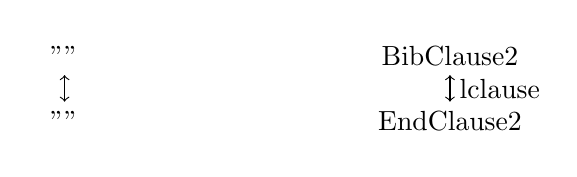
\begin{tikzpicture}
    \matrix (m) [matrix of nodes, row sep=1em, column sep=4em, minimum width=2em]
    {
      \CF{""} & $\Or$ & \CF{BibClause2} \\
      \CF{""} & $\Or$ & \CF{EndClause2} \\
    };
    \path[<->]
    (m-1-1) edge node [left] {} (m-2-1);
    \path[<->]
    (m-1-3) edge node [right] {\CF{lclause}} (m-2-3);
  \end{tikzpicture}

  \CF{lclause : BibClause2 <=> EndClause2}
  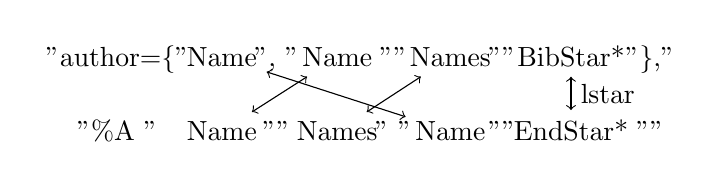
\begin{tikzpicture}
    \matrix (m) [matrix of nodes, row sep=1em, column sep=-.75em]
    {
      \CF{"author=\{"} & \Concat{}\CF{Name}\Concat{} & \CF{", "} &
      \Concat{}\CF{Name}\Concat{} & \CF{""} & \Concat{}\CF{Names}\Concat{} & \CF{""}
      & \Concat{}\CF{BibStar*}\Concat{} & \CF{"\},"}\\
      \CF{"\%A "} & \Concat{}\CF{Name}\Concat{} & \CF{""} &
      \Concat{}\CF{Names}\Concat{} & \CF{" "} & \Concat{}\CF{Name}\Concat{} & \CF{""}
      & \Concat{}\CF{EndStar*}\Concat{} & \CF{""}\\
    };
    \path[<->]
    (m-1-2) edge node [right] {} (m-2-6);
    \path[<->]
    (m-1-4) edge node [left] {} (m-2-2);
    \path[<->]
    (m-1-6) edge node [left] {} (m-2-4);
    \path[<->]
    (m-1-8) edge node [right] {\CF{lstar}} (m-2-8);
  \end{tikzpicture}

  \CF{lstar : BibStar <=> EndStar}
  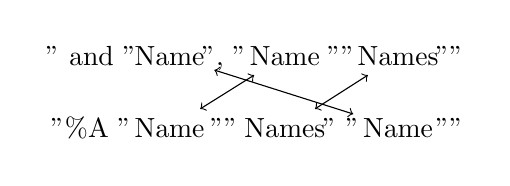
\begin{tikzpicture}
    \matrix (m) [matrix of nodes, row sep=1em, column sep=-.75em]
    {
      \CF{" and "} & \Concat{}\CF{Name}\Concat{} & \CF{", "} &
      \Concat{}\CF{Name}\Concat{} & \CF{""} & \Concat{}\CF{Names}\Concat{} &
      \CF{""}\\
      \CF{"\%A "} & \Concat{}\CF{Name}\Concat{} & \CF{""} &
      \Concat{}\CF{Names}\Concat{} & \CF{" "} & \Concat{}\CF{Name}\Concat{}
      & \CF{""}\\
    };
    \path[<->]
    (m-1-2) edge node [right] {} (m-2-6);
    \path[<->]
    (m-1-4) edge node [left] {} (m-2-2);
    \path[<->]
    (m-1-6) edge node [left] {} (m-2-4);
  \end{tikzpicture}
  \caption{Synthesized Lens Mappings}
\end{figure}

In doing this though, some ambiguity is introduced.  There are two
instances of \CF{Name} present outside a star, so which one should get mapped to
which?  The basic solution would be to map the first to the first, and the
second to the second.  This is not correct, however, as the generated lens for
this will not match the examples.  We can determine which maps to which, as they
must each match the same substrings.  The first \CF{Name} in \CF{DNFBib'}
matches \CF{"Conway"} and the second matches \CF{"John"}.  The first \CF{Name} in
\CF{DNFEndUnroll} matches \CF{"John"} and the second matches \CF{"Conway"}.
This means that the first \CF{Name} in \CF{DNFBib'} must map to the second
\CF{Name} in \CF{DNFEndUnroll}, and vice-versa.  Doing this will generate a lens
that satisfies the type and the examples, shown in Figure~\ref{fig:lens-synth-ex}


% end extended-example

% begin formalisms

\section{DNF Regular Expressions}

% fig:dnf-regex-syntax
\begin{figure}
  \begin{tabular}{l@{\ }l@{\ }c@{\ }l@{\ }>{\itshape\/}r}

    % DNF_REGEX
    (Atoms)& \Atom{},\AtomAlt{} & \GEq{} & \StarOf{\DNFRegex{}} & \StarAtomType{}\\
    (Sequences)& \Sequence{},\SequenceAlt{} & \GEq{} &
                                                       $\SequenceOf{\String_0\SequenceSep\Atom_1\SequenceSep\ldots\SequenceSep\Atom_n\SequenceSep\String_n}$ & \MultiConcatSequenceType{} \\
    (DNF Regexes)& \DNFRegex{},\DNFRegexAlt{} & \GEq{} & $\DNFOf{\Sequence_1\DNFSep\ldots\DNFSep\Sequence_n}$ & \MultiOrDNFRegexType{} \\
  \end{tabular}
  \caption{DNF Regex Syntax} 
  \label{fig:dnf-regex-syntax}
\end{figure}

% fig:dnf-regex-semantics
\begin{figure}
  \begin{tabular}{R@{}L}
    \LanguageOf{\StarOf{\DNFRegex}} = &
                                        \{\String_1\Concat\ldots\Concat\String_n \SuchThat n\in\Nats \wedge \String_i\in\LanguageOf{\DNFRegex}\}\\
    \LanguageOf{\SequenceOf{\String_0\SequenceSep\Atom_1\SequenceSep\ldots\SequenceSep\Atom_n\SequenceSep\String_n}}= &
                                                                                                                        \{\String_0\Concat\StringAlt_1\Concat\ldots\Concat\StringAlt_n\Concat\String_n \SuchThat \StringAlt_i\in\LanguageOf{\Atom_i}\}\\
    \LanguageOf{\DNFOf{\Sequence_1\DNFSep\ldots\DNFSep\Sequence_n}}= &
                                                                       \{\String \SuchThat \String \in \LanguageOf{\Sequence_i} \text{ for some $i\in\RangeIncInc{1}{n}$}\}
  \end{tabular}
  \caption{DNF Regex Semantics}
  \label{fig:dnf-regex-semantics}
\end{figure}

We put our regular expressions into a normal form for synthesis, by putting the
regular expressions into a normal form, called ``disjunctive normal form'' or
``DNF'' regular expressions.
A DNF regular expression is, intuitively, a regular expression with
all terms fully distributed.  This yields an outer layer of regular expressions
separated by $\Or{}$s.  The regular expressions separated by $\Or{}$s are
sequences of strings and $\Star$s all separated by $\Concat{}$s.
The regular expressions beneath the $\Star$s have the same operations applied to
them.
Furthermore, because of the associativity of $\Or{}$ and $\Concat{}$, we
remove associativity information of $\Or{}$ and $\Concat{}$ through a list
representation.  Furthermore, we can further simplify by requiring
base string regular expressions to always appear at fixed locations,
utilizing the fact that $\EmptyString{}$ is the $\Concat$ identity, and
the ability to concatenate strings.
The syntax of the language of DNF regular expressions is formalized in
Figure~\ref{fig:dnf-regex-syntax}.
The shorthand $\SequenceOf{\Atom_1\SequenceSep\ldots\SequenceSep\Atom_n}$
stands for
$\SequenceOf{\EmptyString;\Atom_1;\ldots;\Atom_n;\EmptyString}$, the sequence
with every string being the empty string.

A sequence of strings and atoms is said to be \textit{unambiguously concatenable},
written $\UnambigConcat\SequenceOf{\String_0;\Atom_1;\ldots;\Atom_n;\String_n}$,
if, $\String_i',\StringAlt_i'\in\LanguageOf{\Atom_i}$ for all $i$, then
$\String_0\Concat\String_1'\ldots\Concat\String_n'\String_n=
\String_0\Concat\StringAlt_1'\ldots\Concat\StringAlt_n'\String_n$
implies $\String_i=\StringAlt_i$ for all $i$.  A DNF Regular expression is said
to be \textit{unambiguously iterable} written $\UnambigItOf{\DNFRegex}$ if
$\UnambigItOf{\LanguageOf{\DNFRegex}}$.

The outermost layer is a list of sequences.
This layer intuitively corresponds to the choices involved in regular expression matching, and so represents where the Ors of normal regular expressions exist.
The second layer is a list of alternating strings and stars.
After the choice has been made about what will be expressed,
the base strings and iterated portions remains to be expressed.
This is kept in a normal form by requiring a (possibly empty) string between
each clause.
The clause corresponds to the concatenated data, and is a concatenation of the
fixed data of base strings, and the iterated data of stars.
Finally is the atom, which is a star.
The iteration in atoms correspond to the iteration that takes place in normal stars.
This intuition is formalized by the semantics, given in
Figure~\ref{fig:dnf-regex-semantics}.

\subsection{Expressivity of DNF Regular Expressions}

% fig:dnf-regex-functions
\begin{figure}
  \ConcatSequence{} \OfType{} \ArrowTypeOf{\SequenceType{}}{\ArrowTypeOf{\SequenceType{}}{\SequenceType{}}}\\
  $\ConcatSequenceOf{[\String_0\SequenceSep\Atom_1\SequenceSep\ldots\SequenceSep\Atom_n\SequenceSep\String_n]}{[\StringAlt_0\SequenceSep\AtomAlt_1\SequenceSep\ldots\SequenceSep\AtomAlt_m\SequenceSep\StringAlt_m]}=$\\
  \hspace*{2ex}$[\String_0\SequenceSep\Atom_1\SequenceSep\ldots\SequenceSep\Atom_n\SequenceSep\String_n\Concat\StringAlt_0\SequenceSep\AtomAlt_1\SequenceSep\ldots\SequenceSep\AtomAlt_m\SequenceSep\StringAlt_m]$\\
  \\
  \ConcatDNF{} \OfType{} \ArrowTypeOf{\DNFRegexType{}}{\ArrowTypeOf{\DNFRegexType{}}{\DNFRegexType{}}}\\
  $\ConcatDNFOf{\DNFOf{\Sequence_1\DNFSep\ldots\DNFSep\Sequence_n}}{\DNFOf{\SequenceAlt_1\DNFSep\ldots\DNFSep\SequenceAlt_m}}=$
  \[
    \begin{array}{rcccl}
      \DNFLeft & \ConcatSequenceOf{\Sequence_1}{\SequenceAlt_1}\DNFSep & \cdots
      & \ConcatSequenceOf{\Sequence_1}{\SequenceAlt_m}\DNFSep \\
      \cdots  & \ConcatSequenceOf{\Sequence_n}{\SequenceAlt_1}\DNFSep & \cdots & \ConcatSequenceOf{\Sequence_n}{\SequenceAlt_m} & \DNFRight
    \end{array}
  \]
  \\
  \OrDNF{} \OfType{}
  \ArrowTypeOf{\DNFRegexType{}}{\ArrowTypeOf{\DNFRegexType{}}{\DNFRegexType{}}
  }\\
  $\OrDNFOf{\DNFOf{\Sequence_1\DNFSep\ldots\DNFSep\Sequence_n}}{\DNFOf{\SequenceAlt_1\DNFSep\ldots\DNFSep\SequenceAlt_m}}$=\\
  \hspace*{2ex}$\DNFOf{\Sequence_1\DNFSep\ldots\DNFSep\Sequence_n\DNFSep\SequenceAlt_1\DNFSep\ldots\DNFSep\SequenceAlt_m}$\\
  \\
  (-)\RepeatDNFOfTimes{n} \OfType{} \ArrowTypeOf{\DNFRegexType{}}{\DNFRegexType{}}\\
  $\RepeatDNFOf{0}{\DNFRegex}=\DNFOf{\SequenceOf{\EmptyString}}$\\
  $\RepeatDNFOf{n}{\DNFRegex}=\ConcatDNFOf{\DNFRegex}{\RepeatDNFOf{n-1}{\DNFRegex}}$\\
  \\
  \AtomToDNF{} \OfType
  \ArrowTypeOf{\AtomType{}}{\DNFRegexType{}}\\
  $\AtomToDNFOf{\Atom} = \DNFOf{\SequenceOf{\Atom}}$
  \caption{DNF Regex Functions}
  \label{fig:dnf-regex-functions}
\end{figure}

A DNF regular expression can be created from a regular expression through repeated
application of the distributivity rule, and through removal of association
information.
This process requires some auxiliary definitions
which are defined in Figure~\ref{fig:dnf-regex-functions}.
From these functions, \ToDNFRegex{}, a function which converts a regular expression into
an equivalent DNF regular expression, can be defined.

\begin{definition}
  \leavevmode
  \[
    \begin{array}{rcl}
      \ToDNFRegexOf{\String} & = & \DNFOf{\SequenceOf{\String}}\\
      \ToDNFRegexOf{\emptyset} & = & \DNFOf{}\\
      \ToDNFRegexOf{(\StarOf{\Regex})} & = & \AtomToDNFOf{\StarOf{(\ToDNFRegexOf{\Regex})}}\\
      \ToDNFRegexOf{(\RegexConcat{\Regex_1}{\Regex_2})} & = & \ToDNFRegexOf{\Regex_1} \ConcatDNF \ToDNFRegexOf{\Regex_2}\\
      \ToDNFRegexOf{(\RegexOr{\Regex_1}{\Regex_2})} & = & \ToDNFRegexOf{\Regex_1} \OrDNF \ToDNFRegexOf{\Regex_2}\\
    \end{array}
  \]
\end{definition}

Intuitively, this means that the DNF regular expression with no sequences
corresponds to the empty set.  A single sequence with only a string corresponds
to a base string.  The stars of DNF regular expressions correspond to the stars
of atoms.  The function $\OrDNF$ corresponds to the regular expression
primitive $\Or$.  The function $\ConcatDNF$ corresponds to the regular
expression primitive $\Concat$.  We formalize this in the following theorem.

\begin{restatable}[Completeness of DNF Regexs]{theorem}{dnfrc}
  \label{thm:completeness-dnf-lenses}
  For all regular expressions \Regex{},
  \LanguageOf{\ToDNFRegex(\Regex)}=\LanguageOf{\Regex{}}.
\end{restatable}

Furthermore, we can use prove that language of DNF regular expressions is sound,
and that \ToDNFRegex{} is surjective, by providing a right inverse, $\ToRegex$.

\begin{definition}\leavevmode\\
  $\ToRegexOf{\StarOf{\DNFRegex}} = \StarOf{\ToRegexOf{\DNFRegex}}$\\
  $\ToRegexOf{\SequenceOf{\String_0}} = \String_0$\\
  $\ToRegexOf{\SequenceOf{\String_0\SequenceSep\Atom_1\SequenceSep\ldots
    \SequenceSep\Atom_n\SequenceSep\String_n}} =
  \ToRegexOf{\SequenceOf{\String_0\SequenceSep\Atom_1\SequenceSep
    \ldots\SequenceSep\Atom_{n-1}\SequenceSep\String_{n-1}}}
  \Concat \ToRegexOf{\Atom_n} \Concat \String_{n+1}$\\
  $\ToRegexOf{\DNFOf{}}=\emptyset$\\
  $\ToRegexOf{\DNFOf{\Sequence_1\DNFSep\ldots\DNFSep\Sequence_n}}=
  \ToRegexOf{\DNFOf{\Sequence_1\DNFSep\ldots\DNFSep\Sequence_{n-1}}}
  \Or \ToRegexOf{\Sequence_n}$
\end{definition}

This provides a way to find a regular expression which corresponds to a given
DNF regular expression.  We formalize this correspondence with the theorem
below.

\begin{restatable}[Soundness of DNF Regexs]{theorem}{dnfrs}\leavevmode\\
  \label{thm:soundness-dnf-lenses}
  $\ToDNFRegexOf{\ToRegexOf{\DNFRegex}} = \DNFRegex$
\end{restatable}

\subsection{DNF Regular Expression Rewrites}

In our synthesis algorithm we need to allow for a rewrite system on DNF Regular
Expressions, to search through the equivalences.
Using the star equivalences, rewrites are applied to the stars in a DNF
regular expression, for type-directed synthesis to eventually be applied to the
rewritten regular expressions.  These rewrites are the same ones used in
\textbf{Step 2:  Traversing Equivalences}.

% fig:dnf-regex-rewrites
\begin{figure}
  \begin{mathpar}
    \inferrule[\AtomUnrollstarRule{}]
    {
    }
    {
      \StarOf{\DNFRegex}\RewriteAtom
      \OrDNFOf{\DNFOf{\SequenceOf{\EmptyString}}}{(\ConcatDNFOf{\DNFRegex}{\DNFOf{\SequenceOf{\StarOf{\DNFRegex}}}})}
    }

    \inferrule[\AtomPowerstarRule{}]
    {
      n\in\Nats_{\geq1}
    }
    {
      \StarOf{\DNFRegex}\RewriteAtom
      \ConcatDNFOf{\DNFOf{\SequenceOf{\StarOf{(\RepeatDNFOf{n}{\DNFRegex})}}}}
      {(\RepeatDNFOf{0}{\DNFRegex}\OrDNF\ldots\OrDNF\RepeatDNFOf{n}{\DNFRegex})}
    }

    \inferrule[\DNFRewriteStarRule{}]
    {
      \DNFRegex \Rewrite \DNFRegex'
    }
    {
      \StarOf{\DNFRegex} \RewriteAtom \DNFOf{\SequenceOf{\StarOf{\DNFRegex'}}}
    }

    \inferrule[\AtomDNFRewriteRule{}]
    {
      \Atom_j \RewriteAtom \DNFRegex
    }
    {
      \DNFLeft\Sequence_1\DNFSep\ldots\DNFSep\Sequence_{i-1}\DNFSep\\\\
      \SequenceOf{\String_0\SequenceSep\Atom_1\SequenceSep\ldots\SequenceSep\String_{j-1}\SequenceSep\Atom_j\SequenceSep\String_j\SequenceSep\ldots\SequenceSep\Atom_m\SequenceSep\String_m}\DNFSep\\\\
      \Sequence_{i+1}\DNFSep\ldots\DNFSep\Sequence_n\DNFRight\Rewrite\\\\
      \DNFOf{\Sequence_1\DNFSep\ldots\DNFSep\Sequence_{i-1}} \OrDNF\\
      \DNFOf{\SequenceOf{\String_0\SequenceSep\Atom_1\SequenceSep\ldots\SequenceSep\String_{j-1}}}\ConcatDNF\DNFRegex\ConcatDNF\SequenceOf{\String_j\SequenceSep\ldots\SequenceSep\Atom_m\SequenceSep\String_m} \OrDNF\\
      \DNFOf{\Sequence_{i+1}\DNFSep\ldots\DNFSep\Sequence_n}
    }

    \inferrule[\ReflexivityRule{}]
    {
    }
    {
      \DNFRegex \StarOf{\Rewrite} \DNFRegex
    }

    \inferrule[\TransitivityRule{}]
    {
      \DNFRegex_1 \StarOf{\Rewrite} \DNFRegex_2\\
      \DNFRegex_2 \Rewrite \DNFRegex_3
    }
    {
      \DNFRegex_1 \StarOf{\Rewrite} \DNFRegex_3
    }

  \end{mathpar}
  \caption{DNF Regex Rewrite Rules}
  \label{fig:dnf-regex-rewrites}
\end{figure}


Rewrite rules are provided in Figure~\ref{fig:dnf-regex-rewrites}.
Intuitively, these rewrite rules correspond to expanding a regular expression
into a regular expression which can be used in a more complicated lens.
These rewrite rules are a way of getting around
requiring a full retyping rule, as is present in standard lenses.
These rewrite rules present ways for atoms to be rewritten to DNF regular
expressions.  With the atoms rewritten as regular expressions, \AtomDNFRewriteRule{}
provides a way to combine the rewritten atom into the broader regular
expression.  For example, consider the DNF Regular
Expression $\DNFOf{\SequenceOf{a};\SequenceOf{\StarOf{b};\StarOf{c}};\SequenceOf{d}}$.
This DNF Regular expression matches either $a$, $b^i\Concat c^j$, or $d$.
With the above rules,
$\StarOf{b}\RewriteAtom\DNFOf{\SequenceOf{};\SequenceOf{b\StarOf{b}}}$, which
corresponds to an application of \ProductstarRule{} on $\EmptyString\Concat b$.
This then gets applied in the rules above, leading to the full DNF rewrite
$\DNFOf{\SequenceOf{a};\SequenceOf{\StarOf{b};\StarOf{c}};\SequenceOf{d}}
\Rewrite
\DNFOf{\SequenceOf{a};\SequenceOf{\StarOf{c}};\SequenceOf{b;\StarOf{b};\StarOf{c}};\SequenceOf{d}}$.
This has the same language, but $\SequenceOf{\StarOf{b};\StarOf{c}}$
has been expanded into matching $b^0c^j$ and $b^{i>0}c^j$ separately.
$\StarOf{\Rewrite}$ is used to represent the transitive and
reflexive closure of $\Rewrite$.

Roughly, the \AtomSumstarRule{} rewrite corresponds to \SumstarRule{},
the \AtomUnrollstarRule{} rewrite correspond to \ProductstarRule{}.
and the \DicyclicRewriteStarRule{} rewrite corresponds to \DicyclicityRule{}.
There is no rewrite corresponding to \StarstarRule{}, as that
equivalence introduces ambiguity.
An application of \AtomSumstarRule{} corresponds to doing different things after the last time a certain event has occured, and before the last time that event occurs.
An application of \AtomUnrollstarRule{} corresponds to making a different action for
the empty case of an iteration, the first case of an iteration, and all further cases of the iteration
An application of \DicyclicRewriteStarRule{} corresponds to a reordering of the
variables that corresponds to expressing a ring as an ideal, and the quotient by
that ideal.
\section{DNF Lenses}

% fig:dnf-lens-syntax
\begin{figure}
  \centering
  \begin{tabular}{@{}l@{\ }l@{\ }c@{}l@{\ }>{\itshape\/}r@{}}
    % REGEX
    (Atom Lenses) &\AtomLens{} & \GEq{} & $Iterate(\DNFLens)$ & Iterate\\
    (Sequence Lenses) &\SequenceLens{} & \GEq{} &
                                                  $(\SequenceLensOf{(\String_0,\StringAlt_0)\SequenceLensSep\AtomLens_1\SequenceLensSep\ldots\SequenceLensSep\AtomLens_n\SequenceLensSep(\String_n,\StringAlt_n)}$, &\\
                  & & & $\sigma \in S_n)$ & Clause\SubN{}\\
    (DNF Lenses)& \DNFLens{} & \GEq{} & $(\DNFLensOf{\SequenceLens_1\DNFLensSep\ldots\DNFLensSep\SequenceLens_n}, \sigma \in S_n)$ & DNF\SubN{}\\
  \end{tabular}
  \caption{DNF Lens Syntax}
  \label{fig:dnf-lens-syntax}
\end{figure}

% fig:dnf-lens-semantics
\begin{figure}
  Semantics of Atom Lenses:\\
  $\SemanticsOf{\IterateLensOf{\DNFLens}}$=\\
  \hspace*{3em}$\SetOf{(\String_1\Concat\ldots\Concat\String_n,
    \StringAlt_1\Concat\ldots\Concat\StringAlt_n)\SuchThat
    n\in\NatsZero\BooleanAnd(\String_i,\StringAlt_i)\in\SemanticsOf{\DNFLens}}$\\
  \\
  Semantics of Sequence Lenses:\\
  $\SemanticsOf{(\SequenceLensOf{(\String_0,\StringAlt_0)\SequenceLensSep
      \AtomLens_1\SequenceLensSep\ldots\SequenceLensSep\AtomLens_n
      \SequenceLensSep(\String_n,\StringAlt_n)},\Permutation)}=$\\
  \hspace*{3em}$\SetOf{
    (\String_0\Concat\String_1'\Concat\ldots\Concat\String_n'\Concat\String_n,
    \String_{\Permutation(0)}\Concat\String_{\Permutation(1)}'\Concat\ldots
    \Concat\String_{\Permutation(n)}'\Concat\String_{\Permutation(n)})\SuchThat$\\
    \hspace*{4em}$(\String_i',\StringAlt_i')\in\SemanticsOf{\Atom_i}}$\\
  \\
  Semantics of DNF Lenses:\\
  $\SemanticsOf{(\DNFLensOf{\SequenceLens_1\DNFLensSep\ldots\DNFLensSep
      \SequenceLens_n},\Permutation)}=$\\
  \hspace*{3em}$\SetOf{(\String,\StringAlt)\SuchThat
    (\String,\StringAlt)\in\SequenceLens_i\text{ for some $i$}}$
  \caption{DNF Lens Semantics}
  \label{fig:dnf-lens-semantics}
\end{figure}

% fig:dnf-lens-typing
\begin{figure}
  \centering
  \begin{mathpar}
    \inferrule[\IterateAtomLensRule{}]
    {
      \DNFLens \OfRewritelessType \DNFRegex \Leftrightarrow \DNFRegexAlt
    }
    {
      \IterateLensOf{\DNFLens} \OfRewritelessType \StarOf{\DNFRegex} \Leftrightarrow \StarOf{\DNFRegexAlt}
      (\PutRight\Apply\String_1)\Concat\ldots\Concat(\PutRight\Apply\String_n)
    }

    \inferrule[\SequenceLensRule{}]
    {
      \AtomLens_1 \OfRewritelessType \Atom_1 \Leftrightarrow \AtomAlt_1\\
      \ldots\\
      \AtomLens_n \OfRewritelessType \Atom_n \Leftrightarrow \AtomAlt_n\\
      \sigma \in \PermutationSetOf{n}\\
      \UnambigConcat\SequenceOf{\String_0\SequenceSep\Atom_1\SequenceSep\ldots\SequenceSep\Atom_n\SequenceSep\String_n}\\
      \UnambigConcat\SequenceOf{\StringAlt_0\SequenceSep\AtomAlt_1\SequenceSep\ldots\SequenceSep\AtomAlt_n\SequenceSep\StringAlt_n}
    }
    {
      (\SequenceLensOf{(\String_0,\StringAlt_0)\SequenceLensSep\Atom_1\SequenceLensSep\ldots\SequenceLensSep\Atom_n\SequenceLensSep(\String_n,\StringAlt_n)},\sigma) \OfRewritelessType\\
      \SequenceOf{\String_0\SequenceSep\Atom_1\SequenceSep\ldots\SequenceSep\Atom_n\SequenceSep\String_n}\Leftrightarrow
      \SequenceOf{\StringAlt_0\SequenceSep\AtomAlt_{\sigma(1)}\SequenceSep\ldots\SequenceSep\AtomAlt_{\sigma(n)}\SequenceSep\StringAlt_n}
    }

    \inferrule[\DNFLensRule{}]
    {
      \SequenceLens_1 \OfRewritelessType \Sequence_1 \Leftrightarrow \SequenceAlt_1\\
      \ldots\\
      \SequenceLens_n \OfRewritelessType \Sequence_n \Leftrightarrow \SequenceAlt_n\\
      \sigma \in \PermutationSetOf{n}\\
      i \neq j \Rightarrow \Sequence_{i} \cap \Sequence_{j}=\emptyset\\
      i \neq j \Rightarrow \SequenceAlt_{i} \cap \SequenceAlt_{j}=\emptyset\\
    }
    {
      (\DNFLensOf{\SequenceLens_1\DNFLensSep\ldots\DNFLensSep\SequenceLens_n},\sigma) \OfRewritelessType\\
      \DNFOf{\Sequence_1\DNFSep\ldots\DNFSep\Sequence_n}
      \Leftrightarrow \DNFOf{\SequenceAlt_{\sigma(1)}\DNFSep\ldots\DNFSep\SequenceAlt_{\sigma(n)}}
    }

    \inferrule[\DNFRewriteLensRule{}]
    {
      \DNFRegex' \Rewrite \DNFRegex\\
      \DNFRegexAlt' \Rewrite \DNFRegexAlt\\
      \DNFLens \OfRewritelessType \MapsBetweenTypeOf{\DNFRegex}{\DNFRegexAlt}
    }
    {
      \DNFLens \OfType \MapsBetweenTypeOf{\DNFRegex'}{\DNFRegexAlt'}
    }

  \end{mathpar}
  \caption{DNF Lens Typing}
  \label{fig:dnf-lens-typing}
\end{figure}

Armed with these rewrites, a language for lenses on DNF regular
expressions can be defined.
The syntax is defined in Figure~\ref{fig:dnf-lens-syntax}.
Similarly to the language of lenses, the typing of the lenses
correspond closely to the syntax for the lenses themselves.
The semantics of these DNF lenses are defined in
Figure~\ref{fig:dnf-lens-semantics}.
The typing of these DNF lenses are defined in Figure~\ref{fig:dnf-lens-typing}.
Intuitively, a DNF Regex Lens corresponds roughly to an n-ary version of an ``Or'' lens,
a Sequence Lens corresponds to const lenses for the strings, and a combination of
Concat and Swap lenses for the Atoms.

These DNF lenses only express bijections that are already expressible in the language of lenses.
\begin{restatable}[Soundness of DNF Lenses]{theorem}{dnfls}
  \label{thm:dnfls}
  If there exists a derivation of $\DNFLens \OfType \MapsBetweenTypeOf{\DNFRegex}{\DNFRegexAlt}$,
  then there exists a derivation of $\Lens \OfType \MapsBetweenTypeOf{\Regex}{\RegexAlt}$ such that
  $\LanguageOf{\Regex}=\LanguageOf{\DNFRegex}$,
  $\LanguageOf{\RegexAlt}=\LanguageOf{\DNFRegexAlt}$, and
  $\SemanticsOf{\Lens}=\SemanticsOf{\DNFLens}$.
\end{restatable}

Furthermore, these DNF lenses are able to express a large number of things
expressible in a subset of the language of lenses.
\begin{restatable}[Completeness of DNF Lenses]{theorem}{dnflc}
  \label{thm:dnflc}
  If there exists a derivation for $\Lens \OfType \Regex \Leftrightarrow
  \RegexAlt$,
  then there exists a derivation for
  $\DNFLens \OfType \ToDNFRegexOf{\Regex} \Leftrightarrow \ToDNFRegexOf{\RegexAlt}$
  such that $\SemanticsOf{\Lens}=\SemanticsOf{\DNFLens}$.
\end{restatable}


These lenses are much more suited to synthesis.
The vast majority of the rules have a syntax-directed synthesis algorithm.
We have reduced the dimensions we are searching in from 3 to 2.  Before, given a
specification, multiple rules could be applicable, equivalent regular
expressions would have to be searched through, and regular expressions for
composition would need to be found.
For DNF lenses, only the correct rewrites for the regular expressions, and the
correct permutations for each rule application, must be searched through.
% end formalisms

% begin implementation
\section{Implementation}
We have implemented the lens synthesis algorithm in $n$ lines of OCaml code.

\subsection{Synthesis Overview}
\begin{figure}
  \includegraphics[scale=.5]{synth-lens-schematic.png}
  \label{fig:synth-lens-schematic}
  \caption{Schematic Diagram for Lens Synthesis}
\end{figure}
The synthesis algorithm is shown in a schematic diagram in 
Figure~\ref{fig:synth-lens-schematic}.  The algorithm takes in a pair of
regular expressions, and examples, and converts the regular expressions into
DNF regular expressions, using $\ToDNFRegex{}$.
These then get enqueued, and SynthDNFLens, where the bulk of the work
occurs.

In SynthDNFLens, the highest priority DNF regular expression pair, $\DNFRegex$
and $\DNFRegexAlt$, is popped.
Then, SynthRewritelessDNF sees if there exists DNF lens $\DNFLens
\OfRewritelessType \DNFRegex \Leftrightarrow \DNFRegexAlt$ which satisfies the examples.
If none are found, then each rewrite is applied once on each side of the regular
expressions.
This new list of DNF regular expression doubles is enqueued, and SynthDNFLens is
called again.
If one is found, this DNF lens gets converted to a normal lens, and is returned
to the user.

\subsection{Priority Queue}
The priority queue is implemented using a naive list implementation.
We say that the lower the priority value, the higher the priority.
The priority value of an element is based on the number of expansions that have been
performed, combined with the distance between the two regular expressions, based
on a psuedometric $\Distance$ we have implemented.  This pseudometric is implemented
as the sum of simpler pseudometrics,
$\Distance = \Distance_{size}+\Distance_{dist}$.

$\Distance_{size}$ is defined as merely the difference in the sizes of the DNF
regular expressions.
$\Distance_{size}(\DNFRegex,\DNFRegexAlt)=\AbsOf{\Size(\DNFRegex)-\Size(\DNFRegexAlt)}$

$\Distance_{dist}$ captures how different the distribution of
user defined regular expressions are from each other.
The distribution of user defined regular expressions can be viewed as an
infinite dimensional vector space over the reals, $\VectorSpace{}$.
The basis for this is $\SetOf{1*(\RegexVariable,n) | n\in\Nats, \RegexVariable
  \text{ is a user defined regular expression}}$
DNF regular expressions with variables can map into this with a function by
counting the number of user defined data types present at a given level.
The formal definition for this mapping is given by the function \GetDist{}.

\begin{definition}\leavevmode\\
  \label{def:getdist}
  \begin{tabular}{@{}L@{}L@{}}
    \GetDist(\DNFOf{\Sequence_1;\ldots;\Sequence_n}) &
                                                       =\GetDist(\Sequence_1)+\ldots+\GetDist(\Sequence_n)\\
    \GetDist(\SequenceOf{\String_0;\Atom_1;\ldots;\Atom_n;\String_n}) &
                                                                        =\GetDist(\Atom_1)+\ldots+\GetDist(\Atom_n)\\
    \GetDist(\RegexVariable)&=1*(\RegexVariable,1)\\
    \GetDist(\IterateLensOf{\DNFLens})&=\phi(\GetDist(\DNFLens))
  \end{tabular}

  where $\phi$ is the linear map sending $1*(\RegexVariable,n)$ to
  $1*(\RegexVariable,n+1)$
\end{definition}

Using this, we now have a mapping from regular expressions into the distribution
of user defined regular exprssions.

$\Distance(\DNFRegex,\DNFRegexAlt)=\LOneNorm(\GetDist(\DNFRegex),\GetDist(\DNFRegexAlt))$
where $\LOneNorm$ is the taxicab metric on $\VectorSpace{}$.
The priority of a pair of DNF regular expressions, $(\DNFRegex{},\DNFRegexAlt{})$,
is $\Distance(\DNFRegex{},\DNFRegexAlt{})+8*expansion_{count}$.
Keeping track of expansion count is important as it allows for lower priority
expansions to be eventually popped, instead of getting stuck doing incorrect,
increasingly deep expansions whose DNF regular expressions have a low distance.
\afm{should i do an example, or is that going into too much detail?}
Experimentally, 8 was a good value for how much weight the expansion
count should get in the priority.  It allows for not getting stuck in a local
minima in the search space, while still allowing for the distance to choose the
correct expansion the majority of the time.

\subsection{SynthRewritelessDNF}

While performing type directed synthesis on DNF Regular Expressions, both
synthesizing a rewriteless DNF lens and synthesizing a Sequence lens requires
the generation of a permutation.  Naively searching through all possible
permutations is incredibly inefficient.  If naively searching through all the
rewriteless DNF Lenses between
the DNF regular expressions $\DNFOf{\Sequence_1;\ldots;\Sequence_n}$ and
$\DNFOf{\SequenceAlt_1;\ldots;\SequenceAlt_n}$, there would be $n!$ permutations
processed.

Instead of searching through all possible permutations, a better approach is to
recognize which subcomponents of the types can be mapped to each other, and
create the permutations based on those mappings.  The approach taken for this is
one of further normalization.  A DNF Lens is normalized through ordering its
sequence subcomponents, and a sequence is normalized through ordering its atom
subcomponents.  Through the correct choice of ordering, a rewriteless DNF lens
can be synthesized between $\DNFOf{\Sequence_1;\ldots;\Sequence_n}$ and
$\DNFOf{\SequenceAlt_1;\ldots;\SequenceAlt_n}$ merely through finding a sequence
lens between $\Sequence_i$ and $\SequenceAlt_i$ for all $i$.  Similarly, through
the correct choice of ordering, a a rewriteless Sequence lens can be synthesized
between $\SequenceOf{\String_0;\Atom_1;\ldots;\Atom_n;\String_n}$ and
$\SequenceOf{\StringAlt_0;\AtomAlt_1;\ldots;\AtomAlt_n;\StringAlt_n}$ through
finding atom lenses between $\Atom_i$ and $\AtomAlt_i$ for all $i$.

However, doing these normalizations can change the semantics of the regular
expressions.  To get around this, the alterations taken for normalization can be
remembered, and applied in reverse to the DNF lens to retrieve a lens between
the original DNF regular expressions.

\begin{figure}
  \label{fig:lens-synth-ordering-ex}
  \centering
  \CF{Bib' <=> DNFEndUnroll}
  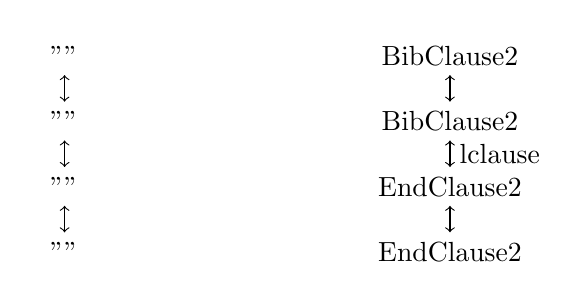
\begin{tikzpicture}
    \matrix (m) [matrix of nodes, row sep=1em, column sep=4em, minimum width=2em]
    {
      \CF{""} & $\Or$ & \CF{BibClause2} \\
      \CF{""} & $\Or$ & \CF{BibClause2} \\
      \CF{""} & $\Or$ & \CF{EndClause2} \\
      \CF{""} & $\Or$ & \CF{EndClause2} \\
    };
    \path[<->]
    (m-1-1) edge node [left] {} (m-2-1);
    \path[<->]
    (m-2-1) edge node [left] {} (m-3-1);
    \path[<->]
    (m-3-1) edge node [left] {} (m-4-1);
    \path[<->]
    (m-1-3) edge node [right] {} (m-2-3);
    \path[<->]
    (m-2-3) edge node [right] {\CF{lclause}} (m-3-3);
    \path[<->]
    (m-3-3) edge node [right] {} (m-4-3);
  \end{tikzpicture}

  \CF{lclause : BibClause2 <=> EndClause2}
  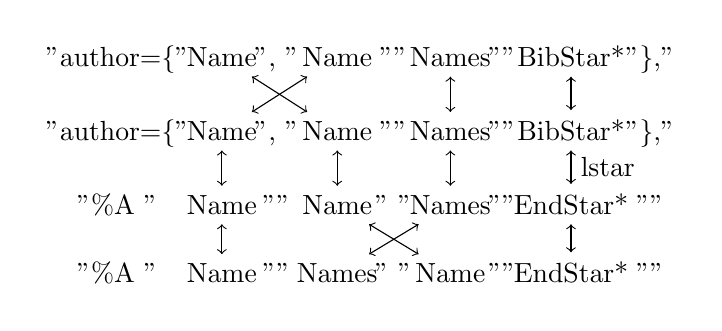
\begin{tikzpicture}
    \matrix (m) [matrix of nodes, row sep=1em, column sep=-.75em]
    {
      \CF{"author=\{"} & \Concat{}\CF{Name}\Concat{} & \CF{", "} &
      \Concat{}\CF{Name}\Concat{} & \CF{""} & \Concat{}\CF{Names}\Concat{} & \CF{""}
      & \Concat{}\CF{BibStar*}\Concat{} & \CF{"\},"}\\
      \CF{"author=\{"} & \Concat{}\CF{Name}\Concat{} & \CF{", "} &
      \Concat{}\CF{Name}\Concat{} & \CF{""} & \Concat{}\CF{Names}\Concat{} & \CF{""}
      & \Concat{}\CF{BibStar*}\Concat{} & \CF{"\},"}\\
      \CF{"\%A "} & \Concat{}\CF{Name}\Concat{} & \CF{""} &
      \Concat{}\CF{Name}\Concat{} & \CF{" "} & \Concat{}\CF{Names}\Concat{} & \CF{""}
      & \Concat{}\CF{EndStar*}\Concat{} & \CF{""}\\
      \CF{"\%A "} & \Concat{}\CF{Name}\Concat{} & \CF{""} &
      \Concat{}\CF{Names}\Concat{} & \CF{" "} & \Concat{}\CF{Name}\Concat{} & \CF{""}
      & \Concat{}\CF{EndStar*}\Concat{} & \CF{""}\\
    };
    \path[<->]
    (m-1-2) edge node [right] {} (m-2-4);
    \path[<->]
    (m-1-4) edge node [right] {} (m-2-2);
    \path[<->]
    (m-1-6) edge node [left] {} (m-2-6);
    \path[<->]
    (m-1-8) edge node [left] {} (m-2-8);
    \path[<->]
    (m-2-2) edge node [right] {} (m-3-2);
    \path[<->]
    (m-2-4) edge node [right] {} (m-3-4);
    \path[<->]
    (m-2-6) edge node [left] {} (m-3-6);
    \path[<->]
    (m-2-8) edge node [right] {\CF{lstar}} (m-3-8);
    \path[<->]
    (m-3-2) edge node [right] {} (m-4-2);
    \path[<->]
    (m-3-4) edge node [right] {} (m-4-6);
    \path[<->]
    (m-3-6) edge node [left] {} (m-4-4);
    \path[<->]
    (m-3-8) edge node [right] {} (m-4-8);
  \end{tikzpicture}

  \CF{lstar : BibStar <=> EndStar}
  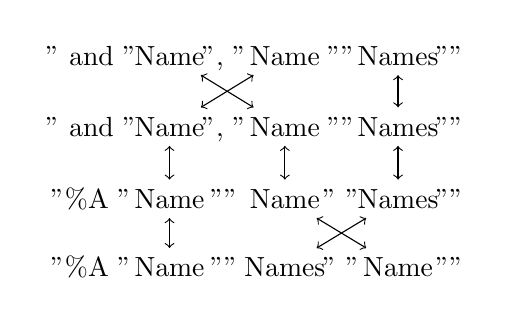
\begin{tikzpicture}
    \matrix (m) [matrix of nodes, row sep=1em, column sep=-.75em]
    {
      \CF{" and "} & \Concat{}\CF{Name}\Concat{} & \CF{", "} &
      \Concat{}\CF{Name}\Concat{} & \CF{""} & \Concat{}\CF{Names}\Concat{} &
      \CF{""}\\
      \CF{" and "} & \Concat{}\CF{Name}\Concat{} & \CF{", "} &
      \Concat{}\CF{Name}\Concat{} & \CF{""} & \Concat{}\CF{Names}\Concat{} &
      \CF{""}\\
      \CF{"\%A "} & \Concat{}\CF{Name}\Concat{} & \CF{""} &
      \Concat{}\CF{Name}\Concat{} & \CF{" "} & \Concat{}\CF{Names}\Concat{}
      & \CF{""}\\
      \CF{"\%A "} & \Concat{}\CF{Name}\Concat{} & \CF{""} &
      \Concat{}\CF{Names}\Concat{} & \CF{" "} & \Concat{}\CF{Name}\Concat{}
      & \CF{""}\\
    };
    \path[<->]
    (m-1-2) edge node [right] {} (m-2-4);
    \path[<->]
    (m-1-4) edge node [left] {} (m-2-2);
    \path[<->]
    (m-1-6) edge node [left] {} (m-2-6);
    \path[<->]
    (m-2-2) edge node [right] {} (m-3-2);
    \path[<->]
    (m-2-4) edge node [left] {} (m-3-4);
    \path[<->]
    (m-2-6) edge node [left] {} (m-3-6);
    \path[<->]
    (m-3-2) edge node [right] {} (m-4-2);
    \path[<->]
    (m-3-4) edge node [left] {} (m-4-6);
    \path[<->]
    (m-3-6) edge node [left] {} (m-4-4);
  \end{tikzpicture}
  \caption{Synthesized Lens Mappings from Orderings}
\end{figure}

Consider the example of synthesizing a lens between \CF{Bib'} and
\CF{DNFEndUnroll}, shown in Figure~\ref{fig:lens-synth-ordering-ex}.  In this,
the subparts of the Bibtex regular expression are ordered from the top, the
subparts of the Endnote regular expression are ordered from the bottom, and the
center matches which subparts map to which.  The final permutation for the DNF
Lens between the two is determined through composition of the orderings done for
normalization.

Unfortunately, while this can find a well typed DNF lens, it doesn't
necessarily find the one that matches the examples.  In the situation where
there are multiple valid sorted orderings, there are multiple different lenses
with potentially different semantics.  For example, in the
synthesis of a lens between \CF{BibStar} and \CF{EndStar}, there are two
instances of \CF{Name}.  Which of these should go first when ordered?  Instead
of iterating through all the possible sortings, and finding one that matches
the examples, we would like to
be able to immediately find only a sorting which satisfies the examples.

The key insight here is that certain invariants must hold for a DNF lens to have
semantics which match the examples.

\begin{enumerate}
\item If a source example string matches one of the clauses during parsing,
  it must be sent to the clause the target example string matches during parsing.
\item If a source example string matches a user defined regular expression during
  parsing, the target must match the exact same string during parsing.
\item If a source example string matches an iteration, then the target must iterate
  the same number of times, and all the invariants must hold for each iterated part.
\end{enumerate}

This is done by joining additional parsing information alongside the regular
expression components, and creating an ordering on DNF Regular expressions
with parsing information.  By attaching additional parsing information,
each \CF{Name} no longer is merely a \CF{Name}, it is \CF{Name} alongside
\CF{"Stephen"} or \CF{"Kleene"}.  With that additional information, the
\CF{Name}s can be ordered, and correctly mapped to the other
\CF{Name}s in a manner that satisfies the examples.


% end implementation


% begin evaluation
\section{Evaluation}
We ran our algorithm on tests validating our ability to handle regular
expression equivalences, tests derived from the Augeus test suite, and from
tests derived from the FlashFill tests.
The values presented are the arithmetic means of 10 test runs.
The tests were run on a 2.5 GHz Intel Core i7 processor, with
16 GB of 1600 MHz DDR3, running Mac OS X Yosemite.

\begin{figure*}
  \centering
  \begin{tabular}{|c|c|c|c|c|}
    \hline
    \bfseries Test & \bfseries ForceExpandTime & \bfseries ForceExpandExamplesRequired
    & \bfseries Computation Time & \bfseries Examples Required
                                   \csvreader[head to column names]{generated-data/data.csv}{}
                                   {\\\hline\Test & \ForceExpandTime & \ForceExpandExamplesRequired & \ComputationTime & \ExamplesRequired}
    \\\hline
  \end{tabular}

\end{figure*}

\subsection{Speed}
\bcp{There should be a subsection discussing the choice of tests -- why did we
  choose the ones we did, in what way are they representative, what are they
  like, maybe giving an example or two of what they look like, which ones are
  easy (and why) and hard (and why)...}
Figure~\ref{fig:runtimes-table} provides the runtime of our algorithm on our
test suite.
In this figure, we want to minimize runtime, as a smaller runtime means we were
able to synthesize very efficiently.
We found that, on many of our difficult examples, our algorithm was able to find
the appropriate lens very quickly.

However, we can also see where the strengths and weaknesses are in our approach.
In particular, our synthesis strategy does quite well on problems that only
include a small number of transformations, even if the number of clauses is
decently large.
This is as expected, for after the appropriate transformations have been found,
the problem of finding the lens between the resulting DNF Regular Expressions
is merely as difficult as ordering the clauses.

For example, the address problem is the second slowest lens to synthesize.
This is because there is a large number of required expansions of user defined
data types, and there are multiple required star transformations.
Furthermore, there are a large number of potential star transformations because
of the large number of stars.
In addition to requiring a relatively deep search, this search is made much
more difficult because of the breadth of the search.
This shows us where our algorithm can hit issues.
When there are a large number of potential transformations, and there are a
large number of required transformations, our search gets more complicated,
and things slow down.

Another place where our synthesis algorithm performs badly is where there is not
only a large number of clauses generated, but they also have a non-identity
lens between them.
For example, the double capitalization problem is another slowest test, despite
being an intuitively easy function to figure out, looking at it as a human.
This is because the algorithm problem has an exponential blow up in terms
of the number of clauses, when there are many regular expressions +d together.
If we take this problem to the logical extremes, we see that the the triple
capitalization problem takes 6.974 seconds, and the quadruple capitalization
problem takes 33 minutes and 54.730 seconds.

\subsection{Importance of Examples}
We wanted to see how many examples were required to synthesize the correct
bijective lens.
However, because of our implicit understanding of the algorithm, we fear we may
choose examples that we know will work well with the synthesis algorithm,
instead of choosing examples that users are likely to.
Because of that, we test the number of examples that it takes to generate the
correct lens, with randomly generated examples.


As we see in Figure~\ref{fig:examples-required-table}, examples are not too
important for synthesizing bijective lenses.\bcp{If that's really the
  conclusion, then maybe we should have written a paper about synthesizing
  bijective lenses {\em without\/} examples!  But I don't think we can
  actually conclude this from the examples we have.  }
\bcp{I still agree with my comment from before.  What I think is really going on
is that we don't have sufficiently interesting tests!!  What sort of tests would
we need, to show where examples are useful}
Because bijective lenses have very few well typed programs, compared to the
number of functions, oftentimes just a few examples is sufficient.
As would be expected, the functions that have to make choices about the
locations of where data goes are those that require more examples.
In particular, the address problem requires more examples, because it must make
choices of where information goes, like which name is the a person's first name,
and which is their last.

\subsection{Importance of User Defined Data Types}

User defined data types are very critical to the algorithm and performance of
the synthesis algorithm.  User defined data types help direct the search of
which expansions should be performed.  Furthermore, they help to reduce the
number of clauses we have to deal with.  There is a potentially exponentially
large blowup in converting regular expressions into DNF form, but keeping
certain portions of the regular expressions abstracted lessens that blowup,
as those regular expressions are kept atomic in converting into DNF form.

User defined data types are also critical in the applications of previously
defined lenses.  We restrict the application of previously defined lenses to
only on user defined data types in the synthesis algorithm.  We then group the
user defined data types based on which have previously defined lenses between
them.  This allows for efficient recognition of when two user defined regular
expressions can be mapped to each other.  Removing the ability to use previously
defined lenses makes certain problems intractable, like (example1, example2,
example3).

While we can simulate the use of user defined data types automatically, by
giving regular expressions which have the same syntax the same user defined data
type, manually inputting them performs better in practice.  This is because the
procedure for automatically creating user defined data types creates far more
data types, which then creates a more complicated search problem.
\bcp{We should also have some discussion of whether the incompleteness of the
  synthesis algorithm (because we didn't do all the equivalences) actually hurts
  us in practice}
% end evaluation

% begin discussion
\subsection{Discussion}

We found that in practice, requiring a user to put in more information for the
synthesis of a string transformation creates a more reliable algorithm.
However, this comes at a few costs.  The user needs to know how to write out
regular expressions.

The largest difficulty in this is the restriction to bijective lenses.
Oftentimes, we find the need to hide information away in some alternate form.
For example, there is oftentimes whitespace in the definition of a regular
expression.  This whitespace must be copied somehow over to the other side.
Oftentimes this requires the use of having a portion of the string dedicated to
holding the whitespace information of the other side.

Another annoyance is the fact that if the correct lens does not exist,
rarely does the tool terminate.  Much of the time it will just spin trying to
perform increasingly complicated transformations to find the correct lens.
A better solution would be to find something close to the correct lens, and have
a user interaction model that supports iterative synthesis.  The user could give
more examples which fix where the program is wrong.
% end discussion


% begin related-work
\section{Related Work}
\subsection{FlashFill}
FlashFill is another string transformation program.  FlashFill takes input and
output examples as its only form of specification.  For FlashFill's primary use
case, providing easy transformations of Excel data, input and output examples as
the only specification makes a lot of sense.  Our tool is intended for use for
programmers to use, who already know regular expressions.  Our tool is oriented
towards a situation where a programmer would check the generated code into a
repository.  From requiring this extra information, our tool is able to handle
synthesize complicated functions that go beyond what FlashFill can synthesize.
For example, given 21 examples of extracting the first author, with the names
reversed, FlashFill still gave incorrect outputs for a number of inputs, even
when those inputs are a similar form to the provided examples.

Furthermore, even if FlashFill were to synthesize the correct program, it would
be foolhardy to check the generated code into a repository.  FlashFill does not
fail on inputs it doesn't know how to handle, rather it tries to provide an
output.  This is different from the generated lenses, which will quickly
fail on inputs that do not match it's intended specification.  Furthermore, the
specification of what inputs should be handled are provided by the user, not
inferred from the examples, giving it more reliability. \afm{talk about how it
  did on bibtex example, more specific on what it did wrong, maybe?}

\subsection{FlashExtract}
FlashExtract is a program that takes an input of a string, and a partial
labeling of substrings within that string, to try to label the rest of the
substrings.  FlashExtract was able to label some amounts of the strings, but was
unable to handle reorderings of the data well.  While it would do well in
extracting data when the data came in the same form, for example, when given a
Bibtex file where the fields come in a specific order, the data would do well,
however, FlashExtract was unable to handle when fields were given in different
orders, even if previous examples in that order were given.
% end related-work

% begin conclusion
\section{Conclusion}

We have coded up an implementation of type-directed synthesis on a domain
specific language of bijective lenses.  This program allows users to input two
regular expressions, and a few input/output examples, and synthesizes a
bijective lens between those regular expressions, matching those input/output
examples.  While lenses are very useful for their guarantees, they are a
difficult domain specific language to code in, in practice.  This program
provides an easier interaction model for the creation of lenses through using
synthesis as the way to interact with the programmer.

This synthesis algorithm is competitive with state of the art tools for
synthesis on strings transformations.  This gain is made through requiring a
larger amount of user interaction with the synthesis algorithm.  However, in the
for this increased interaction, the program provides the capabilities of
synthesizing very complicated transformations, and provides stronger guarantees
about correctness on inputs dissimilar to those provided in the examples.

\subsection{Future Work}
Some of the issues seen in this have already been observed.  For example, in the
quotient lens paper, the issue of having to hack a place in the source string to
move whitespace information from the view to the source was noted.  An extension
we would like to work on would be able to synthesize quotient lenses.

Another approach to having disparate information on each side of the lens is
through the use of symmetric lenses.  This could be another approach to the
whitespace problem.

% end conclusion

\appendix

\ifanon\else
\acks 
% Expeditions in Computer Augmented Program Engineering (ExCAPE, NSF
% Award CCF-1138996).
% Acknowledgments, if needed.
\finish{Write me.  Mention all relevant grants, esp. DARPA.}
\fi

% We recommend abbrvnat bibliography style.

\bibliographystyle{abbrvnat}

% The bibliography should be embedded for final submission.

\bibliography{local}

% Appendices.

\onecolumn
% begin proofs
\section{Proofs}
% proof-dnfrc start
% First we will prove some lemmas.
\begin{lemma}[Equivalence of \ConcatSequence{} and \Concat{}]
  If $\LanguageOf{\Regex}=\LanguageOf{\Sequence}$,
  and $\LanguageOf{\RegexAlt}=\LanguageOf{\SequenceAlt}$,
  then $\LanguageOf{\RegexConcat{\Regex}{\RegexAlt}}=\LanguageOf{\ConcatSequenceOf{\Sequence}{\SequenceAlt}}$.
\end{lemma}
\begin{proof}
  Let $\Sequence=\SequenceOf{\String_0\SequenceSep\Atom_1\SequenceSep\ldots
    \SequenceSep\Atom_n\SequenceSep\String_n}$, and
  let\\ $\SequenceAlt=[\StringAlt_0\SequenceSep\AtomAlt_1\SequenceSep\ldots
  \SequenceSep\AtomAlt_m\SequenceSep\StringAlt_m]$\\
  \begin{tabular}{@{}L@{}L@{}}
    \LanguageOf{\ConcatSequenceOf{\Sequence}{\SequenceAlt}} & = 
                                                              \LanguageOf{\SequenceOf{\String_0\SequenceSep\Atom_1\SequenceSep\ldots
                                                              \SequenceSep\Atom_n\SequenceSep\String_n\Concat\StringAlt_0\SequenceSep{}
                                                              \AtomAlt_1\SequenceSep\ldots\SequenceSep\AtomAlt_m\SequenceSep\StringAlt_m}} \\
                                                            & = 
                                                              \{\String_0\Concat\String_1'\Concat\ldots\Concat\String_n'\Concat\String_n
                                                              \Concat\StringAlt_0\Concat\StringAlt_1'\Concat\ldots
                                                              \Concat\StringAlt_m'\Concat\StringAlt_m \\
                                                            & \hspace{5em} \SuchThat{} \String_i'\in\LanguageOf{\Atom_i} \BooleanAnd{}
                                                              \StringAlt_i'\in\LanguageOf{\AtomAlt_i}\}\\
                                                            & = 
                                                              \{\String\Concat\StringAlt{} \SuchThat{} \String\in\LanguageOf{\Sequence}
                                                              \BooleanAnd{} \StringAlt\in\LanguageOf{\SequenceAlt}\}\\
                                                            & =
                                                              \{\String\Concat\StringAlt{} \SuchThat{} \String\in\LanguageOf{\Regex}
                                                              \BooleanAnd{} \StringAlt\in\LanguageOf{\RegexAlt}\}\\
                                                            & =
                                                              \LanguageOf{\RegexConcat{\Regex}{\RegexAlt}}
  \end{tabular}
\end{proof}

\begin{lemma}[Equivalence of \ConcatDNF{} and \Concat{}]
  \label{lem:cdnfeq}
  If $\LanguageOf{\Regex}=\LanguageOf{\DNFRegex}$,
  and $\LanguageOf{\RegexAlt}=\LanguageOf{\DNFRegexAlt}$,
  then $\LanguageOf{\RegexConcat{\Regex}{\RegexAlt}}=
  \LanguageOf{\ConcatDNFOf{\DNFRegex}{\DNFRegexAlt}}$.
\end{lemma}
\begin{proof}
  Let $\DNFRegex=\DNFOf{\Sequence_0\DNFSep\ldots\DNFSep\Sequence_n}$, and
  let $\DNFRegexAlt=\DNFOf{\SequenceAlt_0\DNFSep\ldots\DNFSep\SequenceAlt_m}$
  \begin{tabular}{@{}L@{}L@{}}
    \LanguageOf{\ConcatDNFOf{\DNFRegex}{\DNFRegexAlt}} & = 
                                                         \LanguageOf{\DNFOf{\ConcatSequenceOf{\Sequence_i}{\SequenceAlt_j}
                                                         \text{ for $i\in\RangeIncInc{1}{n}$, $j\in\RangeIncInc{1}{m}$}}} \\
                                                       & = 
                                                         \{\String\SuchThat \String\in\ConcatSequenceOf{\Sequence_i}{\SequenceAlt_j}\\
                                                       & \hspace{5em}
                                                         \text{ where $i\in\RangeIncInc{1}{n}$, $j\in\RangeIncInc{1}{m}$}\}\\
                                                       & = 
                                                         \{\String\Concat\StringAlt{} \SuchThat{} \String\in\LanguageOf{\Sequence_i}
                                                         \BooleanAnd{} \StringAlt\in\LanguageOf{\SequenceAlt_j}\}\\
                                                       & \hspace{5em}
                                                         \text{ where $i\in\RangeIncInc{1}{n}$, $j\in\RangeIncInc{1}{m}$}\}\\
                                                       & =
                                                         \{\String\Concat\StringAlt{} \SuchThat{} \String\in\LanguageOf{\DNFRegex}
                                                         \BooleanAnd{} \StringAlt\in\LanguageOf{\DNFRegexAlt}\}\\
                                                       & =
                                                         \{\String\Concat\StringAlt{} \SuchThat{} \String\in\LanguageOf{\Regex}
                                                         \BooleanAnd{} \StringAlt\in\LanguageOf{\RegexAlt}\}\\
                                                       & =
                                                         \LanguageOf{\RegexConcat{\Regex}{\RegexAlt}}
  \end{tabular}
\end{proof}

\begin{lemma}[Equivalence of \OrDNF{} and \Or{}]
  \label{lem:odnfeq}
  If $\LanguageOf{\Regex}=\LanguageOf{\DNFRegex}$,
  and $\LanguageOf{\RegexAlt}=\LanguageOf{\DNFRegexAlt}$,
  then $\LanguageOf{\RegexOr{\Regex}{\RegexAlt}}=
  \LanguageOf{\OrDNFOf{\DNFRegex}{\DNFRegexAlt}}$.
\end{lemma}
\begin{proof}
  Let $\DNFRegex=\DNFOf{\Sequence_0\DNFSep\ldots\DNFSep\Sequence_n}$, and
  let $\DNFRegexAlt=\DNFOf{\SequenceAlt_0\DNFSep\ldots\DNFSep\SequenceAlt_m}$
  \begin{tabular}{@{}L@{}L@{}}
    \LanguageOf{\OrDNFOf{\DNFRegex}{\DNFRegexAlt}} & = 
                                                     \LanguageOf{\DNFOf{\Sequence_0\DNFSep\ldots\DNFSep\Sequence_n\DNFSep
                                                     \SequenceAlt_1\DNFSep\ldots\DNFSep\SequenceAlt_m}}\\
                                                   & = 
                                                     \{\String\SuchThat{} \String\in\Sequence_i\vee\String\in\SequenceAlt_j\\
                                                   & \hspace{5em}
                                                     \text{ where $i\in\RangeIncInc{1}{n}$, $j\in\RangeIncInc{1}{m}$}\}\\
                                                   & = 
                                                     \{\String{} \SuchThat{} \String\in\LanguageOf{\DNFRegex}
                                                     \BooleanOr{} \String\in\LanguageOf{\DNFRegexAlt}\}\\
                                                   & =
                                                     \{\String \SuchThat{} \String\in\LanguageOf{\Regex}
                                                     \BooleanOr{} \String\in\LanguageOf{\RegexAlt}\}\\
                                                   & =
                                                     \LanguageOf{\RegexOr{\Regex}{\RegexAlt}}
  \end{tabular}\\
\end{proof}

\dnfrc*
\begin{proof}
  By structural induction.

  Let $\Regex=\String$.
  $\LanguageOf{\ToDNFRegex(\String)}=\LanguageOf{\DNFOf{\SequenceOf{\String}}}=
  \{\String\}=\LanguageOf{\String}$

  Let $\Regex=\emptyset$.
  $\LanguageOf{\ToDNFRegex(\emptyset)}=\LanguageOf{\DNFOf{}} =
  \{\} = \LanguageOf{\emptyset}$.

  Let $\Regex=\StarOf{\Regex'}$.
  By induction assumption, $\LanguageOf{\ToDNFRegex(\Regex')}=
  \LanguageOf{\Regex'}$.\\
  \begin{tabular}{@{}L@{}L@{}}
    \LanguageOf{\ToDNFRegex(\StarOf{\DNFRegex'})} & =
                                                    \LanguageOf{\DNFOf{\SequenceOf{\StarOf{\ToDNFRegex(\Regex')}}}}\\
                                                  & =
                                                    \{\String\SuchThat\String\in
                                                    \LanguageOf{\SequenceOf{\StarOf{\ToDNFRegex(\Regex')}}}\}\\
                                                  & = 
                                                    \{\String\SuchThat{} \String\in\LanguageOf{\StarOf{\ToDNFRegex(\Regex')}}\}\\
                                                  & =
                                                    \{\String_1\Concat\ldots\Concat\String_n\SuchThat{}
                                                    n\in\Nats\\
                                                  & \hspace*{3em}\BooleanAnd\String_i\in\LanguageOf{\ToDNFRegex(\Regex')}\}\\
                                                  & =
                                                    \{\String_1\Concat\ldots\Concat\String_n\SuchThat{}
                                                    n\in\Nats\BooleanAnd\String_i\in\LanguageOf{\Regex'}\}\\
                                                  & = \LanguageOf{\StarOf{\Regex'}}
  \end{tabular}

  Let $\Regex=\RegexConcat{\Regex_1}{\Regex_2}$.
  By induction assumption,
  $\LanguageOf{\ToDNFRegex(\Regex_1)}=\LanguageOf{\Regex_1}$, and
  $\LanguageOf{\ToDNFRegex(\Regex_2)}=\LanguageOf{\Regex_2}$.
  $\ToDNFRegex(\RegexConcat{\Regex_1}{\Regex_2})=
  \ConcatDNFOf{\ToDNFRegex(\Regex_1)}{\ToDNFRegex(\Regex_2)}$.
  By Lemma~\ref{lem:cdnfeq},
  $\RegexConcat{\Regex_1}{\Regex_2}=
  \ConcatDNFOf{\ToDNFRegex(\Regex_1)}{\ToDNFRegex(\Regex_2)}$.

  Let $\Regex=\RegexOr{\Regex_1}{\Regex_2}$.
  By induction assumption,
  $\LanguageOf{\ToDNFRegex(\Regex_1)}=\LanguageOf{\Regex_1}$, and
  $\LanguageOf{\ToDNFRegex(\Regex_2)}=\LanguageOf{\Regex_2}$.
  $\ToDNFRegex(\RegexOr{\Regex_1}{\Regex_2})=
  \OrDNFOf{\ToDNFRegex(\Regex_1)}{\ToDNFRegex(\Regex_2)}$.
  By Lemma~\ref{lem:odnfeq},
  $\RegexOr{\Regex_1}{\Regex_2}=
  \OrDNFOf{\ToDNFRegex(\Regex_1)}{\ToDNFRegex(\Regex_2)}$.
\end{proof}
% proof-dnfrc end



% proof-dnfrs start
% First we will prove some lemmas.
\begin{lemma}
  \label{lem:sequence-rx}
  Let $\SequenceOf{\String_0\SequenceSep\Atom_1\SequenceSep
    \ldots\Atom_n\SequenceSep\String_n}$ be a sequence,
  and\\
  $\ToDNFRegex(\ToRegex(\Atom_i))=\DNFOf{\SequenceOf{\Atom_i}}$.
  Then,\\$\ToDNFRegex(\ToRegex(\SequenceOf{\String_0\SequenceSep\Atom_1\SequenceSep
    \ldots\Atom_n\SequenceSep\String_n}))=$\\
  $\DNFOf{\SequenceOf{\String_0\SequenceSep\Atom_1\SequenceSep
      \ldots\Atom_n\SequenceSep\String_n}}$.
\end{lemma}
\begin{proof}
  By induction on $n$.

  Let $n=0$.
  $\Sequence=\SequenceOf{\String_0}$.\\
  $\ToDNFRegex(\ToRegex(\SequenceOf{\String_0}))=
  \ToDNFRegex(\String_0)=\DNFOf{\SequenceOf{\String_0}}$

  Let $n>0$,
  $\Sequence=\SequenceOf{\String_0\SequenceSep\Atom_1\SequenceSep
    \ldots\Atom_n\SequenceSep\String_n}$.\\
  $\ToDNFRegex(\ToRegex(\SequenceOf{\String_0\SequenceSep\Atom_1\SequenceSep
    \ldots\Atom_n\SequenceSep\String_n}))$\\
  $\ToDNFRegex(\ToRegex(\SequenceOf{\String_0\SequenceSep\Atom_1\SequenceSep
    \ldots\Atom_{n-1}\SequenceSep\String_{n-1}})\Concat\ToRegex(\Atom_n)
  \Concat\String_n)$=\\
  $\ToDNFRegex(\ToRegex(\SequenceOf{\String_0\SequenceSep\Atom_1\SequenceSep
    \ldots\Atom_{n-1}\SequenceSep\String_{n-1}}))
  \ConcatDNF\\
  \ToDNFRegex(\ToRegex(\Atom_n))
  \ConcatDNF\\
  \ToDNFRegex(\String_{n-1})$=
  $\DNFOf{\SequenceOf{\String_0\SequenceSep\Atom_1\SequenceSep
      \ldots\Atom_{n-1}\SequenceSep\String_{n-1}}}
  \ConcatDNF\\
  \DNFOf{\SequenceOf{\Atom_n}}
  \ConcatDNF
  \DNFOf{\SequenceOf{\String_n}}$=
  $\DNFOf{\SequenceOf{\String_0\SequenceSep\Atom_1\SequenceSep
      \ldots\Atom_n\SequenceSep\String_n}}$.
\end{proof}



\begin{lemma}
  \label{lem:dnf-rx}
  Let $\DNFOf{\Sequence_1\DNFSep\ldots\DNFSep\Sequence_n}$ be a sequence,
  and\\ $\ToDNFRegex(\ToRegex(\Sequence_i))=\DNFOf{\Sequence_i}$.
  Then,\\ $\ToDNFRegex(\ToRegex(\DNFOf{\Sequence_1\DNFSep\ldots\DNFSep\Sequence_n}))=
  \DNFOf{\Sequence_1\DNFSep\ldots\DNFSep\Sequence_n}$.
\end{lemma}
\begin{proof}

  By induction on $n$.

  Let $n=0$
  $\ToDNFRegex(\ToRegex(\DNFOf{}))=\ToDNFRegex(\emptyset)=\DNFOf{}$.

  Let $n>0$
  $\ToDNFRegex(\ToRegex(\DNFOf{\Sequence_1\SequenceSep\ldots\SequenceSep\Sequence_n}))=
  \ToDNFRegex(\ToRegex(\DNFOf{\Sequence_1\SequenceSep\ldots\SequenceSep\Sequence_{n-1}})
  \Concat\ToRegex(\Sequence_n))$=
  $\ToDNFRegex(\ToRegex(\DNFOf{\Sequence_1\SequenceSep\ldots\SequenceSep\Sequence_{n-1}}))
  \ConcatDNF\\\ToDNFRegex(\ToRegex(\Sequence_n))$=
  $\DNFOf{\Sequence_1\SequenceSep\ldots\SequenceSep\Sequence_n}$
\end{proof}

\begin{lemma}[Elimination of $\ToDNFRegex\Compose\ToRegex$]\leavevmode
  \begin{enumerate}
  \item $\ToDNFRegex(\ToRegex(\Atom))=\DNFOf{\SequenceOf{\Atom}}$
  \item $\ToDNFRegex(\ToRegex(\Sequence))=\DNFOf{\Sequence}$
  \item $\ToDNFRegex(\ToRegex(\DNFRegex))=\DNFRegex$
  \end{enumerate}
\end{lemma}
\begin{proof}
  By mutual induction

  Let $\StarOf{\DNFRegex}$ be an atom.
  $\ToDNFRegex(\ToRegex(\StarOf{\DNFRegex}))=
  \ToDNFRegex(\StarOf{\ToRegex(\DNFRegex)})=
  \DNFOf{\SequenceOf{\StarOf{\ToDNFRegex(\ToRegex(\DNFRegex))}}}=
  \DNFOf{\SequenceOf{\StarOf{\DNFRegex}}}$

  Let $\SequenceOf{\String_0\SequenceSep\Atom_1\SequenceSep\ldots
    \SequenceSep\Atom_n\SequenceSep\String_n}$ be a sequence.
  $\ToDNFRegex(\ToRegex(\SequenceOf{\String_0\SequenceSep\Atom_1\SequenceSep\ldots
    \SequenceSep\Atom_n\SequenceSep\String_n}))$.
  By induction assumption, for each $\Atom_i$,
  $\ToDNFRegex(\ToRegex(\Atom_i))=\DNFOf{\SequenceOf{\Atom_i}}$.
  By Lemma~\ref{lem:sequence-rx},
  $\ToDNFRegex(\ToRegex(\SequenceOf{\String_0\SequenceSep\Atom_1\SequenceSep\ldots
    \SequenceSep\Atom_n\SequenceSep\String_n}))=
  \DNFOf{\SequenceOf{\String_0\SequenceSep\Atom_1\SequenceSep\ldots
      \SequenceSep\Atom_n\SequenceSep\String_n}}$.

  Let $\DNFOf{\Sequence_1\SequenceSep\ldots\SequenceSep\Sequence_n}$ be a DNF
  regular expression.
  By induction assumption, for each $\Sequence_i$,
  $\ToDNFRegex(\ToRegex(\Sequence_i))=\DNFOf{\Sequence_i}$.
  By Lemma~\ref{lem:dnf-rx},
  $\ToDNFRegex(\ToRegex(\DNFOf{\Sequence_1\SequenceSep\ldots\SequenceSep\Sequence_n}))=
  \DNFOf{\Sequence_1\SequenceSep\ldots\SequenceSep\Sequence_n}$.

\end{proof}
% proof-dnfrs end




% proof-dnfls start
% We will prove a couple of lemmas first.

\begin{lemma}
  \label{lem:unambig-concat-equiv}
  Let $\Language_1,\ldots,\Language_n,\Language_1',\ldots,\Language_m'$ be
  languages. $\SequenceUnambigConcatOf{\Language_1;\ldots;\Language_n}$,
  $\SequenceUnambigConcatOf{\Language_1';\ldots;\Language_m'}$, and
  $\SetOf{\String_1\Concat\ldots\Concat\String_n \SuchThat \String_i \in
    \Language_i} \UnambigConcat
  \SetOf{\String_1\Concat\ldots\Concat\String_m \SuchThat \String_i \in
    \Language_i'}$ if, and only if
  $\SequenceUnambigConcatOf{\Language_1;\ldots;\Language_n;\Language_1';\ldots;\Language_n'}$
\end{lemma}
\begin{proof}
\end{proof}

\begin{lemma}
  \label{lem:unambig-union-equiv}
  Let $A = \SetOf{\Language_1,\ldots,\Language_n}$,
  $B = \SetOf{\Language_1',\ldots,\Language_m'}$,
  $C = \SetOf{\Language_1'',\ldots,\Language_{n+m}''}$, be sets of languages
  Such that $A \Union B = C$.
  $(\BigUnion_{i\in\RangeIncInc{1}{n}}\Language_i) \Intersect
  (\BigUnion_{i\in\RangeIncInc{1}{m}}\Language_i') = \emptyset$,
  for all $i,j\in\RangeIncInc{1}{n}$, $i \neq j \BooleanImplies Language_i \Intersect
  \Language_j = \emptyset$, and for all $i,j\in\RangeIncInc{1}{m}$, $i \neq j
  \BooleanImplies \Language_i \Intersect \Language_j = \emptyset$ if, and only
  if for all $i,j\in\RangeIncInc{1}{n+m}$, $i \neq j \BooleanImplies \Language_i
  \Intersect \Language_j = \emptyset$.
\end{lemma}
\begin{proof}
\end{proof}


\begin{lemma}[Expressibility of Safe Boilerplate Alterations]
  \label{lem:boilerplate-alterations}
  Suppose
  \begin{enumerate}
  \item $\UnambigConcat\SequenceOf{\String_0;\Atom_1;\ldots;\Atom_n;\String_n}$
  \item $\UnambigConcat\SequenceOf{\StringAlt_0;\Atom_1;\ldots;\Atom_n;\StringAlt_n}$
  \end{enumerate}
  Then there exists a lens
  $\Lens \OfType \Regex \Leftrightarrow \RegexAlt$ such that
  \begin{enumerate}
  \item $\Regex = \ToRegex(\SequenceOf{\String_0;\Atom_1;\ldots;\Atom_n;\String_n})$
  \item $\RegexAlt = \ToRegex(\SequenceOf{\StringAlt_0;\Atom_1;\ldots;\Atom_n;\StringAlt_n})$
  \item $\SemanticsOf{\Lens}=\SetOf{(\String,\StringAlt)\SuchThat
      \String=\String_0\Concat\String_1'\Concat\ldots\Concat\String_n'\Concat\String_n
      \BooleanAnd\\
      \hspace*{6.1em}\StringAlt=\StringAlt_0\Concat\String_1'\Concat\ldots\Concat\String_n'\Concat\StringAlt_n
      \BooleanAnd\\
      \hspace*{6.1em}\String_i\in\LanguageOf{\Atom_i}}$
  \end{enumerate}
\end{lemma}
\begin{proof}
  By induction on $n$.

  Let $n=0$.
  Consider the Lens
  \begin{mathpar}
    \inferrule*
    {
    }
    {
      \ConstLensOf{\String_0}{\StringAlt_0} \OfType \String_0 \Leftrightarrow \StringAlt_0
    }
  \end{mathpar}
  By inspection, this satisfies the desired properties.

  Let $n>0$.
  By induction, there exists a lens $\Lens \OfType \Regex \Leftrightarrow \RegexAlt$
  satisfying the desired properties.
  Consider the lens
  \begin{mathpar}
    \inferrule*[left=\Derivation]
    {
      \Lens \OfType \Regex \Leftrightarrow \RegexAlt\\
      \inferrule*
      {
      }
      {
        \ConstLensOf{\String_n}{\StringAlt_n} \OfType \String_n \Leftrightarrow \StringAlt_n
      }
    }
    {
      \ConcatLensOf{\Lens}{\ConstLensOf{\String_n}{\StringAlt_n}}
      \OfType
      \Regex \Concat \String_n \Leftrightarrow
      \RegexAlt \Concat \StringAlt_n
    }

    \inferrule*
    {
      \Derivation\\
      \IdentityLensOf{\ToRegex(\Atom_n)} \OfType \ToRegex(\Atom_n) \Leftrightarrow \ToRegex(\Atom_n)
    }
    {
      \ConcatLensOf{\ConcatLensOf{\Lens}{\ConstLensOf{\String_n}{\StringAlt_n}}}{\IdentityLensOf{\ToRegex(\Atom_n)}}
      \OfType\\
      \Regex \Concat \String_n \Concat \ToRegex(\Atom_n) \Leftrightarrow
      \Regex \Concat \StringAlt_n \Concat \ToRegex(\Atom_n)
    }
  \end{mathpar}
  By inspection, this satisfies the desired properties.
\end{proof}

\begin{lemma}[Creation of Lens from Identity Perm Sequence Lens]
  \label{lem:id-clause}
  Suppose
  \begin{enumerate}
  \item $\Sequence=\SequenceOf{\String_0 ; \Atom_1 ; \ldots ; \Atom_n; \String_n}$
  \item $\SequenceAlt=\SequenceOf{\StringAlt_0 ; \AtomAlt_1 ; \ldots ; \AtomAlt_n ; \StringAlt_n}$
  \item $(\SequenceLensOf{(\String_0,\StringAlt_0);\AtomLens_1 ; \ldots ;
      \AtomLens_n;(\String_n,\StringAlt_n)},id) \OfType
    \Sequence \Leftrightarrow \SequenceAlt$
  \item For each $\AtomLens_i \OfType \Atom_i \Leftrightarrow \AtomAlt_i$,
    there exists a $\Lens_i \OfType \ToRegex(\Atom_i) \Leftrightarrow
    \ToRegex(\AtomAlt_i)$ such that $\SemanticsOf{\Lens_i}=\SemanticsOf{\AtomLens_i}$
  \end{enumerate}
  then there exists a $\Lens \OfType \ToRegex(\Sequence) \Leftrightarrow \ToRegex(\DNFRegexAlt)$ such that
  $\SemanticsOf{\Lens} =
  \SemanticsOf{(\SequenceLensOf{(\String_0,\StringAlt_0);\AtomLens_1 ; \ldots ; \AtomLens_n;(\String_n,\StringAlt_n)},id)}$.
  \begin{proof}
    By induction on $n$.

    Let $n=0$, $(\SequenceLensOf{(\String_0,\StringAlt_0)},id) \OfType
    \SequenceOf{\String_0} \Leftrightarrow \SequenceOf{\StringAlt_0}$.
    Then consider
    \begin{mathpar}
      \inferrule[]
      {
      }
      {
        \ConstLensOf{\String_0}{\StringAlt_0}\OfType\String_0\Leftrightarrow\StringAlt_0
      }
    \end{mathpar}

    $\String_0=\ToRegex(\SequenceOf{\String_0})$,
    and
    $\StringAlt_0=\ToRegex(\SequenceOf{\StringAlt_0})$.
    $\SemanticsOf{\ConstLensOf{\String_0}{\StringAlt_0}}=
    \SetOf{\String_0,\StringAlt_0}=
    \SemanticsOf{\SequenceOf{(\String_0,\StringAlt_0)},id)}$.

    Let $n>0$.
    Let $\Sequence'=\SequenceOf{\String_0\SequenceSep\Atom_1\SequenceSep
      \ldots\SequenceSep\Atom_{n-1}\SequenceSep\String_{n-1}}$,
    and $\SequenceAlt'=\SequenceOf{\StringAlt_0\SequenceSep\AtomAlt_1\SequenceSep
      \ldots\SequenceSep\AtomAlt_{n-1}\SequenceSep\StringAlt_{n-1}}$
    By induction assumption, there exists a typing derivation
    \begin{mathpar}
      \Lens\OfType\ToRegex(\Sequence')\Leftrightarrow\ToRegex(\SequenceAlt')
    \end{mathpar}
    satisfying $\SemanticsOf{\Lens}=\\
    \SemanticsOf{(\SequenceLensOf{(\String_0,\StringAlt_0);\AtomLens_1 ;
        \ldots ; \AtomLens_{n-1};(\String_{n-1},\StringAlt_{n-1})},id)}$

    By problem statement, there exists a typing derivation
    \begin{mathpar}
      \Lens_{\AtomLens_{n}} \OfType
      \ToRegex(\Atom_{n}) \Leftrightarrow \ToRegex(\AtomAlt_{n})
    \end{mathpar}
    satisfying $\SemanticsOf{\Lens_{\Atom_n}}
    =\SemanticsOf{\Atom_n}$.

    Consider the following lens typing
    \begin{mathpar}
      \inferrule*[left=\Derivation{}]
      {
        \Derivation_n\\
        \inferrule*
        {
        }
        {
          \ConstLensOf{\String_n}{\StringAlt_n}
          \OfType
          \String_n \Leftrightarrow \StringAlt_n
        }
      }
      {
        \ConcatLensOf{\Lens_{\AtomLens_n}}{\ConstLensOf{\String_n}{\StringAlt_n}}
        \OfType
        \ToRegex(\Atom_n)\Concat\String_n \Leftrightarrow
        \ToRegex(\AtomAlt_n)\Concat\StringAlt_n
      }

      \inferrule*
      {
        \Lens\OfType\ToRegex(\Sequence) \Leftrightarrow \ToRegex(\SequenceAlt)\\
        \Derivation{}
      }
      {
        \ConcatLensOf
        {\Lens}
        {\ConcatLensOf{\Lens_{\AtomLens_n}}{\ConstLensOf{\String_n}{\StringAlt_n}}}
        \OfType\\
        \ToRegex(\Sequence)\Concat\ToRegex(\Atom_n)\Concat\String_n \Leftrightarrow
        \ToRegex(\SequenceAlt)\Concat\ToRegex(\AtomAlt_n)\Concat\StringAlt_n
      }
    \end{mathpar}

    \SemanticsOf{\ConcatLensOf
      {\Lens}
      {\ConcatLensOf{\Lens_{\AtomLens_n}}{\ConstLensOf{\String_n}{\StringAlt_n}}}}\\
    \hspace*{3em}=\SetOf{(\String,\StringAlt)
      \SuchThat
      \String = \String'\Concat\String''\Concat\String_n\BooleanAnd
      \StringAlt = \StringAlt'\Concat\StringAlt''\Concat\StringAlt_n\BooleanAnd\\
      \hspace*{7em}
      (\String',\StringAlt')\in\SemanticsOf{\Lens}\BooleanAnd
      (\String'',\StringAlt'')\in\SemanticsOf{\Lens_{\AtomLens_n}}}\\
    \hspace*{3em}=\SetOf{
      (\String,\StringAlt)\SuchThat
      \String=
      \String_0\Concat\String_0'\Concat\ldots
      \Concat\String_{n-1}'\Concat\String_{n-1}
      \Concat \String_n \Concat \String_n'\BooleanAnd\\
      \hspace*{7em}\StringAlt=\StringAlt_0\Concat\StringAlt_0'\Concat\ldots
      \Concat\StringAlt_{n-1}'\Concat\StringAlt_{n-1}
      \Concat \StringAlt_n \Concat \StringAlt_n'\BooleanAnd\\
      \hspace*{7em}\String_i'\in\Atom_i\BooleanAnd\StringAlt_i'\in\AtomAlt_i}\\
    \hspace*{3em}=\SemanticsOf{(\SequenceLensOf{(\String_0,\StringAlt_0);\AtomLens_1 ;
        \ldots ; \AtomLens_n;(\String_n,\StringAlt_{n-1})},id)}
  \end{proof}
\end{lemma}

\begin{theorem}[Unambiguity of $\Sep$]
  Let $\Alphabet$ be an alphabet.  Let $\Alphabet_{\Sep}=\Alphabet\Union\SetOf{\Sep}$,
  where \Sep{} is a character not in \Alphabet{}.
  If $\Language_1, \ldots,
  \Language_n$, are languages in $\StarOf{\Alphabet}$, then
  $\UnambigConcat\SequenceOf{\LanguageOf{\Sep};\Language_1;\LanguageOf{\Sep};
    \ldots;\LanguageOf{\Sep};\Language_n;\LanguageOf{\Sep}}$.
\end{theorem}
\begin{proof}
  We prove this by induction on $n$.

  Let $n=0$.  $\UnambigConcat\SequenceOf{\LanguageOf{\Sep}}$, as
  $\UnambigConcat\SequenceOf{\Language}$, for any language $\Language$.

  Let $n>0$.
  Let $\String_i, \StringAlt_i\in\Language_i$ for all $i\in\RangeIncInc{1}{n}$,
  and let $\Sep\String_1\Sep\ldots\Sep\String_n\Sep=\Sep\StringAlt_1\Sep\ldots\Sep\StringAlt_n\Sep$.
  We want to show that $\String_n\Sep=\StringAlt_n\Sep$.
  If they were not equal, then one string is strictly contained in the other, say without
  loss of generality $\String_n\Sep$ is strictly contained in $\StringAlt_n\Sep$.
  Because of that $\Sep\String_n\Sep$ is contained in $\StringAlt_n\Sep$, so $\Sep$
  is contained in $\StringAlt_n\in\StarOf{\Sigma}$.  This is a contradiction,
  as $\Sep\notin\Sigma$, so we know $\String_n\Sep=\StringAlt_n\Sep$, and so $\String_n=\StringAlt_n$.
  This means that
  $\Sep\String_0\Sep\ldots\Sep\String_{n-1}\Sep=\Sep\StringAlt_0\Sep\ldots\Sep\StringAlt_{n-1}$,
  so by induction, I know $\String_i=\StringAlt_i$ for all $i$.
\end{proof}

\begin{definition}[Adjacent Swapping Permutation]
  Let $\sigma_{i} \in S_n$ be the permutation where
  $\sigma_{i}(i) = i+1$, $\sigma_{i}(i+1) = i$, $\sigma_{i}(k) = k$
  when $k\neq i$, and $k\neq i+1$.
\end{definition}

\begin{lemma}[Expressibility of Adjacent Swapping Permutation Lens]
  \label{lem:adj-perm-exp}
  Suppose
  \begin{enumerate}
  \item $\sigma_i$ is an adjacent element swapping permutation
  \item $\SequenceOf{\Sep;\Atom_1;\Sep\ldots\Sep;\Atom_n;\Sep}$ is a sequence with
    all base strings equal to $\Sep$.
  \end{enumerate}
  Then there exists a typing of a lens $\Lens \OfType \Regex \Leftrightarrow \RegexAlt$ such that
  \begin{enumerate}
  \item $\LanguageOf{\Regex}=\LanguageOf{[\Sep;\Atom_1;\ldots;\Atom_n;\Sep]}$
  \item $\LanguageOf{\RegexAlt}=\LanguageOf{[\Sep;\Atom_{\sigma_i(1)};\ldots;\Atom_{\sigma_i(n)};\Sep]}$
  \item $\SemanticsOf{\Lens}=
    \SetOf{(\String,\StringAlt)\SuchThat\String=\Sep\Concat\String_1\Concat\Sep\Concat\ldots\Concat\Sep\Concat\String_n\Concat\Sep
      \BooleanAnd\\
      \hspace*{6em}\StringAlt=\Sep\Concat\String_{\sigma_i(1)}\Concat\Sep\Concat\ldots\Concat\Sep\Concat\String_{\sigma_i(n)}\Sep\BooleanAnd\\
      \hspace*{6em}\String_i\in\LanguageOf{\Atom_i}}$
  \end{enumerate}
  \begin{proof}
    By the soundness of regular expressions, define regular expressions
    $\Regex_1, \Regex_2, \Regex_3, \Regex_4$ as
    $\Regex_1=\ToRegex([\Sep;\Atom_1;\ldots;\Atom_{i-1};\Sep])$,
    $\Regex_2=\ToRegex(\Atom_i)$,
    $\Regex_3=\ToRegex(\Atom_{i+1})$, and
    $\Regex_4=\ToRegex([\Sep;\Atom_{i+1};\ldots;\Atom_{n};\Sep])$.
    Consider the following deduction\bcp{I find these deductions a bit heavy and
      hard to read, but I guess I can get used to them.  }
    \afm{Anybody have suggestions for better deduction package?}
    \begin{mathpar}

      \inferrule*[left=\Derivation{}]
      {
        \inferrule*
        {
        }
        {
          \IdentityLensOf{\Sep} \OfType \Sep \Leftrightarrow \Sep
        }
        \inferrule*
        {
        }
        {
          \IdentityLensOf{\Regex_3} \OfType \Regex_3 \Leftrightarrow \Regex_3
        }
      }
      {
        \SwapLensOf{\IdentityLensOf{\Sep}}{\IdentityLensOf{\Regex_3}} \OfType 
        \Sep\Concat\Regex_3 \Leftrightarrow \Regex_3\Concat\String_i
      }

      \inferrule*[left=\Derivation{}']
      {
        \inferrule*
        {
        }
        {
          \IdentityLensOf{\Regex_2} \OfType \Regex_2 \Leftrightarrow \Regex_2
        }\\
        \Derivation
      }
      {
        \SwapLensOf{\IdentityLensOf{\Regex_2}}{\SwapLensShortOf{\IdentityLensShortOf{\Sep}}{\IdentityLensShortOf{\Regex_3}}} \OfType
        \Regex_2\Concat\Sep\Concat\Regex_3 \Leftrightarrow \Regex_3\Concat\Sep\Concat\Regex_2
      }

      \inferrule*[left=\Derivation{}'']
      {
        \inferrule*
        {
        }
        {
          \IdentityLensOf{\Regex_1} \OfType \Regex_1 \Leftrightarrow \Regex_1
        }\\
        \Derivation{}'
      }
      {
        \ConcatLensOf{\IdentityLensOf{\Regex_1}}{\SwapLensShortOf{\IdentityLensShortOf{\Regex_2}}{\SwapLensShortOf{\IdentityLensShortOf{\Sep}}{\IdentityLensShortOf{\Regex_3}}}} \OfType\\
        \Regex_1\Concat\Regex_2\Concat\Sep\Concat\Regex_3 \Leftrightarrow \Regex_1\Concat\Regex_3\Concat\Sep\Concat\Regex_2
      }


      \inferrule*
      {
        \Derivation{}''\\
        \inferrule*
        {
        }
        {
          \IdentityLensOf{\Regex_4} \OfType \Regex_4 \Leftrightarrow \Regex_4
        }
      }
      {
        \ConcatLensOf{\ConcatLensShortOf{\IdentityLensShortOf{\Regex_1}}{\SwapLensShortOf{\IdentityLensShortOf{\Regex_2}}{\SwapLensShortOf{\IdentityLensShortOf{\Sep}}{\IdentityLensShortOf{\Regex_3}}}}}{\IdentityLensOf{\Regex_4}} \OfType\\
        \Regex_1\Concat\Regex_2\Concat\Sep\Concat\Regex_3\Concat\Regex_4 \Leftrightarrow \Regex_1\Concat\Regex_3\Concat\Sep\Concat\Regex_2\Concat\Regex_4
      }
    \end{mathpar}

    By inspection, the final lens
    $\ConcatLensShortOf{\ConcatLensShortOf{\IdentityLensShortOf{\Regex_1}}{\SwapLensShortOf{\IdentityLensShortOf{\Regex_2}}{\SwapLensShortOf{\IdentityLensShortOf{\Sep}}{\IdentityLensShortOf{\Regex_3}}}}}{\IdentityLensShortOf{\Regex_4}} \OfType
    \Regex_1\Concat\Regex_2\Concat\Sep\Concat\Regex_3\Concat\Regex_4 \Leftrightarrow \Regex_1\Concat\Regex_3\Concat\Sep\Concat\Regex_2\Concat\Regex_4$
    satisfies $\LanguageOf{\Regex_1\Concat\Regex_2\Concat\String_i\Concat\Regex_3\Concat\Regex_4}=\LanguageOf{\SequenceOf{\Sep;\Atom_1;\Sep;\ldots;\Sep;\Atom_n;\Sep}}$ and
    $\LanguageOf{\Regex_1\Concat\Regex_3\Concat\String_i\Concat\Regex_2\Concat\Regex_4}=\LanguageOf{\SequenceOf{\Sep;\Atom_{\sigma_i(1)};\ldots;\Atom_{\sigma_i(n)};\Sep}}$
    and has the desired semantics of swapping the strings at spots $i$ and $i+1$.
  \end{proof}
\end{lemma}

\begin{lemma}[Expressibility of Adjacent Swapping Permutation Composition]
  \label{lem:adj-comp-perm-exp}
  Suppose
  \begin{enumerate}
  \item $\sigma=\sigma_{i_1}\Compose\ldots\Compose\sigma_{i_m}$ 
  \item $\SequenceOf{\Sep;\Atom_1;\Sep\ldots\Sep;\Atom_n;\Sep}$ is a sequence with
    all base strings equal to $\Sep$.
  \end{enumerate}
  Then there exists a typing of a lens $\Lens \OfType \Regex \Leftrightarrow \RegexAlt$ such that
  \begin{enumerate}
  \item $\LanguageOf{\Regex}=\LanguageOf{[\Sep;\Atom_1;\ldots;\Atom_n;\Sep]}$
  \item $\LanguageOf{\RegexAlt}=\LanguageOf{[\Sep;\Atom_{\sigma(1)};\ldots;\Atom_{\sigma(n)};\Sep]}$
  \item $\SemanticsOf{\Lens}=
    \SetOf{(\String,\StringAlt)\SuchThat\String=\Sep\Concat\String_1\Concat\Sep\Concat\ldots\Concat\Sep\Concat\String_n\Concat\Sep
      \BooleanAnd\\
      \hspace*{6em}\StringAlt=\Sep\Concat\String_{\sigma(1)}\Concat\Sep\Concat\ldots\Concat\Sep\Concat\String_{\sigma(n)}\Sep\BooleanAnd\\
      \hspace*{6em}\String_i\in\LanguageOf{\Atom_i}}$
  \end{enumerate}
  \begin{proof}
    By induction on $m$.

    Let $m=0$.  Then $\sigma=\Identity$.  Consider the lens
    $\IdentityLensOf{\ToRegex(\SequenceOf{\Sep;\Atom_1;\Sep\ldots\Sep;\Atom_n;\Sep})} \OfType
    \ToRegex(\SequenceOf{\Sep;\Atom_1;\Sep\ldots\Sep;\Atom_n;\Sep}) \Leftrightarrow
    \ToRegex(\SequenceOf{\Sep;\Atom_1;\Sep\ldots\Sep;\Atom_n;\Sep})$.
    By inspection, this lens satisfies the requirements.

    Let $m>0$.  Let $\sigma'=\sigma_{i_1}\Compose\ldots\Compose\sigma_{i_{m-1}}$.
    Let $\Lens \OfType \Regex \Leftrightarrow \RegexAlt$ be the lens obtained by an
    application of the induction assumption on $\sigma'$.
    Let $\Lens_m \OfType \RegexAlt' \Leftrightarrow \RegexAlt''$ be the lens obtained by
    an application of Lemma~\ref{lem:adj-perm-exp} to the permutation $\sigma_m$ and
    the sequence $\SequenceOf{\Sep;\Atom_{\sigma'(1)};\ldots;\Atom_{\sigma'(n)};\Sep}$.
    From the induction assumption and the previous lemmas,
    we know $\LanguageOf{\RegexAlt}=
    \LanguageOf{\SequenceOf{\Sep;\Atom_{\sigma'(1)};\ldots;\Atom_{\sigma'(n)};\Sep}}=
    \LanguageOf{\RegexAlt'}$.
    Consider the following Lens typing

    \begin{mathpar}
      \inferrule*
      {
        \inferrule*
        {
          \Lens \OfType \Regex \Leftrightarrow \RegexAlt\\
          \LanguageOf{\RegexAlt}=\LanguageOf{\RegexAlt'}
        }
        {
          \Lens \OfType \Regex \Leftrightarrow \RegexAlt'
        }\\
        \Lens_m \OfType \RegexAlt' \Leftrightarrow \RegexAlt''
      }
      {
        \ComposeLensOf{\Lens_m}{\Lens} \OfType \Regex \Leftrightarrow \RegexAlt''
      }
    \end{mathpar}

    The language of \Regex{} is already as desired, and
    $\LanguageOf{\RegexAlt''}=
    \LanguageOf{\SequenceOf{\Sep;\Atom_{\sigma_m\Compose\sigma'(1)};\ldots;\Atom_{\sigma_m\Compose\sigma'(n)}}}=
    \LanguageOf{\SequenceOf{\Sep;\Atom_{\sigma(1)};\ldots;\Atom_{\sigma(n)}}}$, as desired.
    Furthermore, the composition of the lenses composes the permutations of strings,
    giving the semantics as desired.
  \end{proof}
\end{lemma}

\begin{lemma}[Expressibility of Permutation]
  \label{lem:perm-exp}
  Suppose
  \begin{enumerate}
  \item $\sigma$ is a permutation in $S_n$
  \item $\SequenceOf{\Sep;\Atom_1;\Sep\ldots\Sep;\Atom_n;\Sep}$ is a sequence with
    all base strings equal to $\Sep$.
  \end{enumerate}
  Then there exists a typing of a lens $\Lens \OfType \Regex \Leftrightarrow \RegexAlt$ such that
  \begin{enumerate}
  \item $\LanguageOf{\Regex}=\LanguageOf{[\Sep;\Atom_1;\ldots;\Atom_n;\Sep]}$
  \item $\LanguageOf{\RegexAlt}=\LanguageOf{[\Sep;\Atom_{\sigma(1)};\ldots;\Atom_{\sigma(n)};\Sep]}$
  \item $\SemanticsOf{\Lens}=
    \SetOf{(\String,\StringAlt)\SuchThat\String=\Sep\Concat\String_1\Concat\Sep\Concat\ldots\Concat\Sep\Concat\String_n\Concat\Sep
      \BooleanAnd\\
      \hspace*{6em}\StringAlt=\Sep\Concat\String_{\sigma(1)}\Concat\Sep\Concat\ldots\Concat\Sep\Concat\String_{\sigma(n)}\Sep\BooleanAnd\\
      \hspace*{6em}\String_i\in\LanguageOf{\Atom_i}}$
  \end{enumerate}
\end{lemma}
\begin{proof}
  By algebra, any permutation can be expressed as the composition of adjacent swapping permutations.
  As such, $\sigma=\sigma_{i_1}\Compose\ldots\Compose\sigma_{i_m}$ for some adjacency swapping
  permutations $\sigma_{i_j}$.
  By Lemma~\ref{lem:adj-comp-perm-exp}, we obtain a lens with the properties desired.
\end{proof}

\begin{lemma}[Creation of Lens from Identity Perm DNF Lens]
  \label{lem:id-dnf}
  Suppose
  \begin{enumerate}
  \item $\DNFRegex = \DNFOf{\Sequence_1 ; \ldots ; \Sequence_n}$
  \item $\DNFRegexAlt = \DNFOf{\SequenceAlt_1 ; \ldots ; \SequenceAlt_n}$
  \item $(\DNFLensOf{\SequenceLens_1 ; \ldots ; \SequenceLens_n},id) \OfType
    \DNFRegex \Leftrightarrow \DNFRegexAlt$
  \item For each $\SequenceLens_i \OfType \Sequence_i \Leftrightarrow \SequenceAlt_i$,
    there exists a $\Lens_i$ such that $\SemanticsOf{\Lens_i}=\SemanticsOf{\SequenceLens_i}$.
  \end{enumerate}
  then there exists a $\Lens \OfType \ToRegex(\DNFRegex) \Leftrightarrow \ToRegex(\DNFRegexAlt)$ such that $\SemanticsOf{\Lens} = \SemanticsOf{([\SequenceLens_1 ; \ldots ; \SequenceLens_n],id)}$.
  \begin{proof}
    By induction on n

    Let $n=0$.
    $\DNFLensOf{} \OfType \DNFOf{} \Leftrightarrow \DNFOf{}$.  Then consider
    \begin{mathpar}
      \inferrule*
      {
      }
      {
        \IdentityLensOf{\ToRegex(\DNFOf{})} \OfType
        \ToRegex(\DNFOf{}) \Leftrightarrow \ToRegex(\DNFOf{})
      }
    \end{mathpar}
    This has the desired typing, and
    $\SemanticsOf{\IdentityLensOf{\ToRegex(\DNFOf{})}}
    =\SemanticsOf{\IdentityLensOf{\emptyset}}
    =\SetOf{}=\SemanticsOf{\DNFLensOf{}}$.

    Let $n>0$.
    Let $\DNFRegex' = \DNFOf{\Sequence_1;\ldots;\Sequence_{n-1}}$, and
    $\DNFRegexAlt' = \DNFOf{\SequenceAlt_1;\ldots;\SequenceAlt_{n-1}}$.
    By induction assumption, there exists a derivation of 
    $\Lens \OfType \ToRegex(\DNFRegex') \Leftrightarrow \ToRegex(\DNFRegexAlt')$.
    By problem statement, there exists a typing derivation
    $\Lens_n \OfType \ToRegex(\Sequence_n) \Leftrightarrow \ToRegex(\SequenceAlt_n)$
    Consider the following derivation
    \begin{mathpar}
      \inferrule*
      {
        \Lens \OfType \ToRegex(\DNFRegex') \Leftrightarrow \ToRegex(\DNFRegexAlt')\\
        \Lens_n \OfType \ToRegex(\Sequence_n) \Leftrightarrow \ToRegex(\SequenceAlt_n)
      }
      {
        \OrLensOf{\Lens_n}{\Lens} \OfType \RegexOr{\ToRegex(\DNFRegex')}{\ToRegex(\Sequence_n)} \Leftrightarrow \RegexOr{\ToRegex(\DNFRegexAlt')}{\ToRegex(\Sequence_n)}
      }
    \end{mathpar}
    $\SemanticsOf{\OrLensOf{\Lens}{\Lens_n}}=\SetOf{(\String,\StringAlt)\SuchThat
      (\String,\StringAlt)\in\Lens\BooleanOr(\String,\StringAlt)\in\Lens_n}$\\
    \hspace*{4.6em}$=\SetOf{(\String,\StringAlt)\SuchThat
      (\String,\StringAlt)\in\DNFLensOf{\SequenceLens_1;\ldots;\SequenceLens_{n-1}}\\
      \hspace*{8em}\BooleanOr(\String,\StringAlt)\in\DNFLensOf{\SequenceLens_n}}$\\
    \hspace*{4.6em}$=\SetOf{(\String,\StringAlt)\SuchThat
      (\String,\StringAlt)\in\SequenceLens_i}$.
  \end{proof}
\end{lemma}

\begin{lemma}[Ineffectiveness of Permutation on DNF Regex Semantics]
  \label{lem:dnfr-perm-sem-ineffective}
  Let $\sigma\in S_n$, and $\DNFOf{\Sequence_1\ldots\Sequence_n}$ be a DNF regex.
  $\LanguageOf{\DNFOf{\Sequence_1;\ldots;\Sequence_n}}=
  \LanguageOf{\DNFOf{\Sequence_{\sigma(1)};\ldots;\Sequence_{\sigma(n)}}}$.
\end{lemma}
\begin{proof}
  By inspection.
\end{proof}

\begin{lemma}[Ineffectiveness of Permutation on DNF Lens Semantics]
  \label{lem:dnfl-perm-sem-ineffective}
  Let $\sigma\in S_n$, and
  $(\DNFLensOf{\SequenceLens_1;\ldots;\SequenceLens_n},\Identity) \OfType
  \DNFOf{\Sequence_1;\ldots;\Sequence_n} \Leftrightarrow
  \DNFOf{\SequenceAlt_1;\ldots;\SequenceAlt_n}$ be a typing of a DNF lens with
  an identity permutation.
  $\SemanticsOf{(\DNFLensOf{\SequenceLens_1;\ldots;\SequenceLens_n},\Identity)}
  =\SemanticsOf{(\DNFLensOf{\SequenceLens_1;\ldots;\SequenceLens_n},\sigma)}$
\end{lemma}
\begin{proof}
  By inspection
\end{proof}

\begin{lemma}[Rewrites Respecting Language]
  \label{lem:rrl}
  If $\DNFRegex\Rewrite\DNFRegexAlt$, then $\LanguageOf{\DNFRegex}=\LanguageOf{\DNFRegexAlt}$
\end{lemma}
\begin{proof}
  Each of the rewrite rules are merely an application of one direction of one of
  the regular expression star equivalences.
\end{proof}

\begin{lemma}[Soundness of DNF, Sequence, and Atom Lenses]\leavevmode
  \label{lem:dnfcal}
  \begin{enumerate}
  \item Let \DNFRegex{} and \DNFRegexAlt{} be two dnf regular expressions, and $\DNFLens \OfType \DNFRegex \Leftrightarrow \DNFRegexAlt$.  Then there exists a \Lens{} such that $\Lens \OfType \ToRegex(\DNFRegex) \Leftrightarrow \ToRegex(\DNFRegexAlt)$, \SemanticsOf{\Lens}=\SemanticsOf{\DNFLens}

  \item Let \Sequence{} and \SequenceAlt{} be two clauses, and $\SequenceLens \OfType \Sequence \Leftrightarrow \SequenceAlt$.  Then there exists a \Lens{} such that $\Lens \OfType \ToRegex(\Sequence) \Leftrightarrow \ToRegex(\SequenceAlt)$, \SemanticsOf{\Lens}=\SemanticsOf{\SequenceLens}.

  \item Let \Atom{} and \AtomAlt{} be two atoms, and $\AtomLens \OfType \Atom \Leftrightarrow \AtomAlt$.  Then there exists a \Lens{}, such that $\Lens \OfType \ToRegex(\Atom) \Leftrightarrow \ToRegex(\AtomAlt)$, \SemanticsOf{\Lens}=\SemanticsOf{\AtomLens}.
  \end{enumerate}
  \begin{proof}
    By mutual induction on the structure of the DNF Regex, Sequence, and
    Atom lenses typing.\\ 
    \\
    Let $\DNFLens \OfType \DNFRegex \Leftrightarrow \DNFRegexAlt$ be formed from an
    application of\\$\DNFRewriteLensRule{}$.
    \begin{mathpar}
      \inferrule*
      {
        \DNFLens \OfType \DNFRegex' \Leftrightarrow \DNFRegexAlt'\\
        \DNFRegex' \Rewrite \DNFRegex\\
        \DNFRegexAlt' \Rewrite \DNFRegexAlt
      }
      {
        \DNFLens \OfType \DNFRegex \Leftrightarrow \DNFRegexAlt
      }
    \end{mathpar}
    By induction assumption, there exists a
    $\Lens \OfType \ToRegex(\DNFRegex') \Leftrightarrow \ToRegex(\DNFRegexAlt')$,
    and from Lemma~\ref{lem:rrl}, we know
    $\LanguageOf{\DNFRegex}=\LanguageOf{\DNFRegex'}$, and
    $\LanguageOf{\DNFRegexAlt}=\LanguageOf{\DNFRegexAlt'}$.
    Consider the derivation
    \begin{mathpar}
      \inferrule*
      {
        \Lens \OfType \ToRegex(\DNFRegex') \Leftrightarrow \ToRegex(\DNFRegexAlt')\\
        \LanguageOf{\ToRegex(\DNFRegex')} = \LanguageOf{\ToRegex(\DNFRegex)}\\
        \LanguageOf{\ToRegex(\DNFRegexAlt')} = \LanguageOf{\ToRegex(\DNFRegexAlt)}
      }
      {
        \Lens \OfType \ToRegex(\DNFRegex) \Leftrightarrow \ToRegex(\DNFRegexAlt)
      }
    \end{mathpar}
    This has the desired typing, and by induction assumption, has the desired semantics.\\
    \\
    Let $(\DNFLensOf{\SequenceLens_1;\ldots;\SequenceLens_n},\sigma) \OfType \DNFOf{\Sequence_1;\ldots;\Sequence_n} \Leftrightarrow \DNFOf{\SequenceAlt_{\sigma(1)};\ldots;\SequenceAlt_{\sigma(n)}}$ be formed from an application of $\DNFLensRule$.
    By Induction assumption, for each $\SequenceLens_i \OfType \Sequence_i \Leftrightarrow \SequenceAlt_i$ there exists a $\Lens_i \OfType \ToRegex(\Sequence_i) \Leftrightarrow \ToRegex(\SequenceAlt_i)$.\\
    By Lemma~\ref{lem:id-dnf} there exists a $\Lens \OfType \ToRegex(\DNFOf{\Sequence_1;\ldots;\Sequence_{n}}) \Leftrightarrow \ToRegex(\DNFOf{\SequenceAlt_1;\ldots;\SequenceAlt_{n}})$ such that $\SemanticsOf{\Lens}=\SemanticsOf{([\SequenceLens_1;\ldots\SequenceLens_n],id)}$,
    By Lemma~\ref{lem:dnfl-perm-sem-ineffective},
    $\SemanticsOf{(DNFOf{\SequenceLens_1;\ldots;\SequenceLens_n},id)}=
    \SemanticsOf{(\DNFOf{\SequenceLens_1;\ldots;\SequenceLens_n},\sigma)}$.
    By Lemma~\ref{lem:dnfr-perm-sem-ineffective},
    $\LanguageOf{\DNFOf{\SequenceAlt_1;\ldots;\SequenceAlt_n}}=
    \LanguageOf{\DNFOf{\SequenceAlt_{\sigma(1)};\ldots;\SequenceAlt_{\sigma(n)}}}$.
    Consider the following typing

    \begin{mathpar}
      \inferrule*
      {
        \Lens \OfType \ToRegex(\DNFOf{\Sequence_1;\ldots;\Sequence_{n}}) \Leftrightarrow \ToRegex(\DNFOf{\SequenceAlt_1;\ldots;\SequenceAlt_{n}})\\
        \LanguageOf{\ToRegex(\DNFOf{\SequenceAlt_1;\ldots;\SequenceAlt_{n}})} =
        \LanguageOf{\ToRegex(\DNFOf{\SequenceAlt_{\sigma(1)};\ldots;\SequenceAlt_{\sigma(n)}})}
      }
      {
        \Lens \OfType \ToRegex(\DNFOf{\Sequence_1;\ldots;\Sequence_{n}}) \Leftrightarrow \ToRegex(\DNFOf{\SequenceAlt_{\sigma(1)};\ldots;\SequenceAlt_{\sigma(n)}})
      }
    \end{mathpar}
    This has the typing and semantics as desired.\\
    \\
    Let $(\SequenceLensOf{(\String_0,\StringAlt_0);\AtomLens_1;\ldots;\AtomLens_n;(\String_n,\StringAlt_n)},\sigma \in S_n) \OfType \SequenceOf{\String_0 ; \Atom_1 ; \ldots ; \Atom_n ; \String_n} \Leftrightarrow \SequenceOf{\StringAlt_0; \AtomAlt_{\sigma(1)} ; \ldots ; \AtomAlt_{\sigma(n)} ; \StringAlt_n}$ be formed from an
    application of\\$\SequenceLensRule{}$.
    By induction assumption, for each
    $\AtomLens_i \OfType \Atom_i \Leftrightarrow \AtomAlt_i$ there exists a
    $\Lens_i \OfType \ToRegex(\Regex_i) \Leftrightarrow \ToRegex(\RegexAlt_i)$.
    By Lemma~\ref{lem:id-clause}, there exists a $\Lens \OfType \Regex \Leftrightarrow \RegexAlt$ such that $\SemanticsOf{\Lens}=\SemanticsOf{([(\String_0,\StringAlt_0);\AtomLens_1;\ldots;\AtomLens_n;(\String_n,\StringAlt_n)],id)}$,
    $\Regex=\ToRegex(\SequenceOf{\String_0;\Atom_1;\ldots;\Atom_n;\String_n})$, and
    $\RegexAlt=\ToRegex(\SequenceOf{\StringAlt_0;\AtomAlt_1;\ldots;\AtomAlt_n;\StringAlt_n})$.
    Define $\RegexAlt_{\Sep}$ as $\ToRegex(\SequenceOf{\Sep;\AtomAlt_1;\ldots;\AtomAlt_n;\Sep})$.
    By Lemma~\ref{lem:boilerplate-alterations}, there exists a
    $\Lens' \OfType \RegexAlt \Leftrightarrow \RegexAlt_{\Sep}$, with semantics of
    merely changing the boilerplate.
    By Lemma~\ref{lem:perm-exp}, there exists a $\Lens'' \OfType \RegexAlt_{\Sep}'
    \Leftrightarrow \RegexAlt_{\Sep}''$ where
    $\SemanticsOf{\RegexAlt_{\Sep}'}=\SemanticsOf{\RegexAlt_{\Sep}}$ and 
    $\SemanticsOf{\RegexAlt_{\Sep}''}=\SemanticsOf{\SequenceOf{\Sep; \AtomAlt_{\sigma(1)} ; \ldots ; \AtomAlt_{\sigma(n)} ; \Sep}}$.
    Lastly, with Lemma~\ref{lem:boilerplate-alterations}, there exists a
    $\Lens''' \OfType \RegexAlt_{\Sep}'' \Leftrightarrow \RegexAlt'$, where
    $\RegexAlt = \ToRegex(\SequenceOf{\StringAlt_0; \AtomAlt_{\sigma(1)} ; \ldots ; \AtomAlt_{\sigma(n)} ; \StringAlt_n})$.
    Through composition of all these lenses, we finally get a lens with the desired type
    and semantics.\\
    \\
    Let $\IterateLensOf{\DNFLens} \OfType \StarOf{\DNFRegex} \Leftrightarrow \StarOf{\DNFRegexAlt}$
    be introduced through an application of \IterateAtomLensRule{}.
    From induction assumption, I know that there exists $\Lens \OfType \Regex \Leftrightarrow \RegexAlt$, such that
    $\SemanticsOf{\DNFLens}=\SemanticsOf{\Lens}$,
    \Regex=\ToRegex(\DNFRegex), and
    $\RegexAlt=\ToRegex(\DNFRegexAlt)$.\\
    Consider $\IterateLensOf{\Lens} \OfType \StarOf{\Regex} \Leftrightarrow \StarOf{\RegexAlt}$.\\
    By definition, $\StarOf{\Regex}$ and $\StarOf{\RegexAlt}$ are $\ToRegex(\StarOf{\DNFRegex})$
    and $\ToRegex(\StarOf{\Regex})$, respectively.

    \begin{tabular}{RcL}
      \SemanticsOf{\IterateLensOf{\Lens}} & = &
                                                \SetOf{(\String_0\ldots\String_n,\StringAlt_0\ldots\StringAlt_n)\SuchThat
                                                (\String_i,\StringAlt_i)\in\SemanticsOf{\Lens}}\\
                                          & = &
                                                \SetOf{(\String_0\ldots\String_n,\StringAlt_0\ldots\StringAlt_n)\SuchThat
                                                (\String_i,\StringAlt_i)\in\SemanticsOf{\DNFLens}}\\
                                          & = &
                                                \SemanticsOf{\IterateLensOf{\DNFLens}}
    \end{tabular}
  \end{proof}
\end{lemma}

\dnfls*
\begin{proof}

  The soundess of DNF lenses follows immediatley from Lemma~\ref{lem:dnfcal}

\end{proof}

\begin{theorem}[Strong DNF Lens Soundness]
  Let $\DNFLens \OfType \DNFRegex \Leftrightarrow \DNFRegexAlt$, be the typing
  of a DNF lens $\DNFLens$.
  and let $\Regex$ and $\RegexAlt$ be regular expressions, such that
  $\LanguageOf{\DNFRegex}=\LanguageOf{\Regex}$,
  and $\LanguageOf{\DNFRegexAlt}=\LanguageOf{\RegexAlt}$.
  There exists a lens $\Lens : \Regex \Leftrightarrow \RegexAlt$, such that
  $\SemanticsOf{\Lens}=\SemanticsOf{\DNFLens}$.
\end{theorem}

\begin{proof}
  By Theorem~\ref{thm:dnfls}, there exist regular expressions $\Regex'$,
  $\RegexAlt'$, such that there exists a lens $\DNFLens$ such there is the
  derivation for a typing.
  \begin{mathpar}
    \inferrule[]
    {
      \Derivation{}
    }
    {
      \DNFLens \OfType \Regex' \Leftrightarrow \RegexAlt'
    }
  \end{mathpar}
  \SemanticsOf{\DNFLens}=\SemanticsOf{\Lens},
  \LanguageOf{\Regex'}=\LanguageOf{\DNFRegex},
  and \LanguageOf{\RegexAlt'}=\LanguageOf{\DNFRegexAlt'}.
  Because of this, $\Regex'\equiv\Regex$, and $\RegexAlt'\equiv\RegexAlt$.
  Consider the typing
  \begin{mathpar}
    \inferrule*
    {
      \inferrule*
      {
        \Derivation{}
      }
      {
        \DNFLens \OfType \Regex' \Leftrightarrow \RegexAlt'
      }\\
      \Regex'\equiv\Regex\\
      \RegexAlt'\equiv\RegexAlt
    }
    {
      \DNFLens \OfType \Regex \Leftrightarrow \RegexAlt
    }
  \end{mathpar}

  This satisfies the needed requirements!
\end{proof}
% proof-dnfls end


% proof-dnflc start
% We will prove a couple of lemmas first.

\begin{lemma}[DNF Lens Inversion]
  \label{lem:dnf-lens-inversion}
  \leavevmode
  \begin{enumerate}
  \item If $\DNFLens \OfType \DNFRegex \Leftrightarrow \DNFRegexAlt$, then there
    exists some $\DNFRegex'$, $\DNFRegexAlt'$ such that
    $\DNFLens \OfRewritelessType \DNFRegex' \Leftrightarrow \DNFRegexAlt'$,
    $\DNFRegex \StarOf{\Rewrite} \DNFRegex'$, and $\DNFRegexAlt
    \StarOf{\Rewrite} \DNFRegexAlt'$.
  \item If $\DNFLens \OfRewritelessType \DNFRegex \Leftrightarrow \DNFRegexAlt$,
    then there exists some $n\in\NatsZero$, $\Sequence_1,\ldots,\Sequence_n$,
    $\SequenceAlt_1,\ldots\SequenceAlt_n$, $\sigma\in\PermutationSetOf{n}$, and
    $\SequenceLens_1;\ldots;\SequenceLens_n$ such that
    for all $i\in\RangeIncInc{1}{n}$, $\SequenceLens_i \OfRewritelessType
    \Sequence_i \Leftrightarrow \SequenceAlt_i$, $\DNFLens =
    (\DNFLensOf{\Sequence_0;\ldots;\Sequence_n},\sigma)$, $\DNFRegex =
    \DNFOf{\Sequence_1;\ldots;\Sequence_n}$, and $\DNFRegexAlt =
    \DNFOf{\SequenceAlt_{\sigma(1)};\ldots;\SequenceAlt_{\sigma(n)}}$.
  \item If $\SequenceLens \OfRewritelessType \Sequence \Leftrightarrow
    \SequenceAlt$, there exists some $n \in \NatsZero$,
    $\Atom_1,\ldots,\Atom_n$, $\AtomAlt_1,\ldots,\AtomAlt_n$,
    $String_0,\ldots,\String_n$, $\StringAlt_0,\ldots,\StringAlt_n$,
    $\sigma\in\PermutationSetOf{n}$, and $\AtomLens_1,\ldots,\AtomLens_n$ such that
    for all $i\in\RangeIncInc{1}{n}$, $\AtomLens_i \OfRewritelessType \Atom_i
    \Leftrightarrow \AtomAlt_i$, $\SequenceLens =
    (\SequenceLensOf{(\String_0,\StringAlt_0);\Atom_1;\ldots;
      \Atom_n;(\String_n,\StringAlt_n)},\sigma)$, $\Sequence =
    \SequenceOf{\String_0;\Atom_1;\ldots;\Atom_n;\String_n}$, and $\SequenceAlt =
    \SequenceOf{\StringAlt_0;\Atom_{\sigma(1)};\ldots;\Atom_{\sigma(n)};\StringAlt_n}$.
  \item If $\AtomLens \OfRewritelessType \Atom \Leftrightarrow \AtomAlt$, then
    there exists some $\DNFLens$, $\DNFRegex$, $\DNFRegexAlt$, such that
    $\DNFLens \OfRewritelessType \DNFRegex \Leftrightarrow \DNFRegexAlt$,
    $\AtomLens = \IterateLensOf{\DNFLens}$, $\Atom = \StarOf{\DNFRegex}$, and
    $\AtomAlt = \StarOf{\DNFRegexAlt}$.
  \end{enumerate}
\end{lemma}
\begin{proof}\leavevmode
  \begin{enumerate}
  \item
    Let $\DNFLens \OfType \DNFRegex \Leftrightarrow \DNFRegexAlt$.  The
    only rule that introduces a typing of this form is
    \DNFRewriteLensRule{}.  Because of this, there
    exists some $\DNFRegex'$, $\DNFRegexAlt'$ such that
    $\DNFLens \OfRewritelessType \DNFRegex' \Leftrightarrow \DNFRegexAlt'$,
    $\DNFRegex \StarOf{\Rewrite} \DNFRegex'$, and $\DNFRegexAlt
    \StarOf{\Rewrite} \DNFRegexAlt'$, to build up the typing
    \[
      \inferrule*
      {
        \DNFLens \OfRewritelessType \DNFRegex' \Leftrightarrow \DNFRegexAlt'\\
        \DNFRegex \StarOf{\Rewrite} \DNFRegex'\\
        \DNFRegexAlt \StarOf{\Rewrite} \DNFRegexAlt'
      }
      {
        \DNFLens \OfType \DNFRegex \Leftrightarrow \DNFRegexAlt
      }
    \]
  \item
    Let $\DNFLens \OfRewritelessType \DNFRegex \Leftrightarrow \DNFRegexAlt$.
    The only rule that introduces a typing of this form is \DNFLensRule{}.
    Because of this there exists some $n\in\NatsZero$, $\Sequence_1,\ldots,\Sequence_n$,
    $\SequenceAlt_1,\ldots\SequenceAlt_n$, $\sigma\in\PermutationSetOf{n}$, and
    $\SequenceLens_1;\ldots;\SequenceLens_n$ such that
    for all $i\in\RangeIncInc{1}{n}$, $\SequenceLens_i \OfRewritelessType
    \Sequence_i \Leftrightarrow \SequenceAlt_i$, $\DNFLens =
    (\DNFLensOf{\Sequence_0;\ldots;\Sequence_n},\sigma)$, $\DNFRegex =
    \DNFOf{\Sequence_1;\ldots;\Sequence_n}$, $\DNFRegexAlt =
    \DNFOf{\SequenceAlt_{\sigma(1)};\ldots;\SequenceAlt_{\sigma(n)}}$,
    $i \neq j \BooleanImplies \Sequence_i \Intersect \Sequence_j = \emptyset$,
    and
    $i \neq j \BooleanImplies \SequenceAlt_i \Intersect \SequenceAlt_j = \emptyset$,
    to build up the typing
    \[
      \inferrule*
      {
        \SequenceLens_i \OfRewritelessType \Sequence_i \Leftrightarrow
        \SequenceAlt_i\\
        i \neq j \BooleanImplies \Sequence_i \Intersect \Sequence_j =
        \emptyset\\
        i \neq j \BooleanImplies \SequenceAlt_i \Intersect \SequenceAlt_j =
        \emptyset
      }
      {
        \DNFLens \OfRewritelessType \DNFRegex \Leftrightarrow \DNFRegexAlt
      }
    \]
  \item
    Let $\SequenceLens \OfRewritelessType \Sequence \Leftrightarrow \SequenceAlt$.
    The only rule that introduces a typing of this form is \SequenceLensRule{}.
    Because of this there exists some $n \in \NatsZero$,
    $\Atom_1,\ldots,\Atom_n$, $\AtomAlt_1,\ldots,\AtomAlt_n$,
    $String_0,\ldots,\String_n$, $\StringAlt_0,\ldots,\StringAlt_n$,
    $\sigma\in\PermutationSetOf{n}$, and $\AtomLens_1,\ldots,\AtomLens_n$ such that
    for all $i\in\RangeIncInc{1}{n}$, $\AtomLens_i \OfRewritelessType \Atom_i
    \Leftrightarrow \AtomAlt_i$, $\SequenceLens =
    (\SequenceLensOf{(\String_0,\StringAlt_0);\Atom_1;\ldots;
      \Atom_n;(\String_n,\StringAlt_n)},\sigma)$, $\Sequence =
    \SequenceOf{\String_0;\Atom_1;\ldots;\Atom_n;\String_n}$, and $\SequenceAlt =
    \SequenceOf{\StringAlt_0;\Atom_{\sigma(1)};\ldots;\Atom_{\sigma(n)};\StringAlt_n}$
    to build up the typing
    \[
      \inferrule*
      {
        \AtomLens_i \OfRewritelessType \Atom_i \Leftrightarrow \AtomAlt_i\\
        \SequenceUnambigConcatOf{\String_0;\Atom_1;\ldots;\Atom_n;\String_n}\\
        \SequenceUnambigConcatOf{\StringAlt_0;\AtomAlt_{\sigma(1)};\ldots;\AtomAlt_{\sigma(n)};\StringAlt_n}
      }
      {
        (\SequenceLensOf{(\String_0,\StringAlt_0);\Atom_1;\ldots;
          \Atom_n;(\String_n,\StringAlt_n)},\sigma) \OfRewritelessType
        \SequenceOf{\String_0;\Atom_1;\ldots;\Atom_n;\String_n} \Leftrightarrow
        \SequenceOf{\StringAlt_0;\Atom_{\sigma(1)};\ldots;\Atom_{\sigma(n)};\StringAlt_n}
      }
    \]
  \item
    Let $\AtomLens \OfRewritelessType \Atom \Leftrightarrow \AtomAlt$.
    The only rule that introduces a typing of this form is
    \IterateAtomLensRule{}.
    Because of this, there exists some $\DNFLens$, $\DNFRegex$, $\DNFRegexAlt$, such that
    $\DNFLens \OfRewritelessType \DNFRegex \Leftrightarrow \DNFRegexAlt$,
    $\AtomLens = \IterateLensOf{\DNFLens}$, $\Atom = \StarOf{\DNFRegex}$, and
    $\AtomAlt = \StarOf{\DNFRegexAlt}$ to build up the typing
    \[
      \inferrule*
      {
        \DNFLens \OfRewritelessType \DNFRegex \Leftrightarrow \DNFRegexAlt\\
        \UnambigItOf{DNFRegex}\\
        \UnambigItOf{DNFRegexAlt}
      }
      {
        \IterateLensOf{\DNFLens} \OfRewritelessType
        \StarOf{\DNFRegex} \Leftrightarrow \StarOf{\DNFRegexAlt}
      }
    \]
  \end{enumerate}
\end{proof}

\begin{lemma}
  \label{lem:dnf-or-assoc}
  $(\DNFRegex_1 \OrDNF \DNFRegex_2) \OrDNF \DNFRegex_3 =
  \DNFRegex_1 \OrDNF (\DNFRegex_2 \OrDNF \DNFRegex_3)$
\end{lemma}
\begin{proof}
\end{proof}

\begin{lemma}
  \label{lem:dnf-concat-assoc}
  $(\DNFRegex_1 \ConcatDNF \DNFRegex_2) \ConcatDNF \DNFRegex_3 =
  \DNFRegex_1 \ConcatDNF (\DNFRegex_2 \ConcatDNF \DNFRegex_3)$
\end{lemma}
\begin{proof}
\end{proof}

\begin{lemma}
  \label{lem:dnf-or-concat-dist-left}
  $\DNFRegex_1 \ConcatDNF (\DNFRegex_2 \OrDNF \DNFRegex_3) =
  (\DNFRegex_1 \ConcatDNF \DNFRegex_2) \OrDNF (\DNFRegex_1 \ConcatDNF \DNFRegex_3)$
\end{lemma}
\begin{proof}
\end{proof}

\begin{lemma}
  \label{lem:dnf-or-concat-dist-right}
  $(\DNFRegex_1 \OrDNF \DNFRegex_2) \ConcatDNF \DNFRegex_3 =
  (\DNFRegex_1 \ConcatDNF \DNFRegex_3) \OrDNF (\DNFRegex_2 \ConcatDNF \DNFRegex_3)$
\end{lemma}
\begin{proof}
\end{proof}

\begin{lemma}
  \label{lem:dnf-or-identity-left}
  $\DNFOf{} \OrDNF \DNFRegex_1 = \DNFRegex_1$
\end{lemma}
\begin{proof}
\end{proof}

\begin{lemma}
  \label{lem:dnf-or-identity-right}
  $\DNFRegex_1 \OrDNF \DNFOf{} = \DNFRegex_1$
\end{lemma}
\begin{proof}
\end{proof}

\begin{lemma}
  \label{lem:dnf-concat-identity-left}
  $\DNFOf{\SequenceOf{\EmptyString}} \ConcatDNF \DNFRegex = \DNFRegex$
\end{lemma}
\begin{proof}
\end{proof}

\begin{lemma}
  \label{lem:dnf-concat-identity-right}
  $\DNFRegex \ConcatDNF \DNFOf{\SequenceOf{\EmptyString}} = \DNFRegex$
\end{lemma}
\begin{proof}
\end{proof}

\begin{lemma}
  \label{lem:dnf-lens-concat-identity-left}
  $\DNFLensOf{\SequenceLensOf{(\EmptyString,\EmptyString)}} \ConcatDNFLens
  \DNFLens = \DNFLens$
\end{lemma}
\begin{proof}
\end{proof}

\begin{lemma}
  \label{lem:dnf-lens-concat-identity-right}
  $\DNFLens \ConcatDNFLens
  \DNFLensOf{\SequenceLensOf{(\EmptyString,\EmptyString)}} = \DNFLens$
\end{lemma}
\begin{proof}
\end{proof}

\begin{definition}[Permutation Functions]\leavevmode\\
  $\ConcatPermutation{} \OfType{}
  \ArrowTypeOf{\PermutationSetOf{n}}
  {\ArrowTypeOf{\PermutationSetOf{m}}{\PermutationSetOf{n+m}}}$\\
  $(\ConcatPermutationOf{\sigma_1}{\sigma_2})(i) =
  \begin{cases*}
    \sigma_1(i) & if $i \leq n$\\
    \sigma_2(i-n)+n & otherwise
  \end{cases*}$\\
  \\\\
  $\SwapPermutation{} \OfType{}
  \ArrowTypeOf{\PermutationSetOf{n}}
  {\ArrowTypeOf{\PermutationSetOf{m}}{\PermutationSetOf{n+m}}}$\\
  $(\SwapPermutationOf{\sigma_1}{\sigma_2})(i) =
  \begin{cases*}
    \sigma_1(i)+m & if $i \leq n$\\
    \sigma_2(i-n) & otherwise
  \end{cases*}$\\
  \\\\
  $\DistributePermutation{} \OfType{}
  \ArrowTypeOf{\PermutationSetOf{n}}
  {\ArrowTypeOf{\PermutationSetOf{m}}{\PermutationSetOf{n\times m}}}$\\
  $(\DistributePermutationOf{\sigma_1}{\sigma_2})(i,j) =
  (\sigma_1(i),\sigma_2(j))$
\end{definition}

\begin{definition}[DNF Lens Functions]\leavevmode\\
  $\ConcatSequenceLens{} \OfType{}
  \ArrowTypeOf{\SequenceLensType{}}
  {\ArrowTypeOf{\SequenceLensType{}}{\SequenceLensType{}}}$\\
  $\ConcatSequenceLensOf
  {(\SequenceLensOf{(\String_0,\StringAlt_0);\AtomLens_1;\ldots;\AtomLens_n;(\String_n,\StringAlt_n)},\sigma_1)}
  {(\SequenceLensOf{(\String_0',\StringAlt_0');\AtomLens_1';\ldots;\AtomLens_m';(\String_m',\StringAlt_m')},\sigma_2)}=$\\
  \hspace*{2ex}$(\SequenceLensOf{(\String_0,\StringAlt_0);\AtomLens_1;\ldots;\AtomLens_n;
    (\String_n\Concat\String_0',\StringAlt_n\Concat\StringAlt_0');\AtomLens_1';
    \ldots;\AtomLens_m';(\String_m',\StringAlt_m')},\ConcatPermutationOf{\sigma_1}{\sigma_2})$\\
  \\
  \\$\SwapSequenceLens{} \OfType{}
  \ArrowTypeOf{\SequenceLensType{}}
  {\ArrowTypeOf{\SequenceLensType{}}{\SequenceLensType{}}}$\\
  Let $\String_i'' =
  \begin{cases*}
    \String_i & for $i \in \RangeIncInc{0}{n-1}$ \\
    \String_n \Concat \String_0 & for $i = n$\\
    \String_i' & for $i \in \RangeIncInc{n+1}{n+m}$
  \end{cases*}$
  Let $\StringAlt_i'' =
  \begin{cases*}
    \StringAlt_i' & for $i \in \RangeIncInc{0}{m-1}$ \\
    \StringAlt_m' \Concat \StringAlt_0 & for $i = m$\\
    \StringAlt_i & for $i \in \RangeIncInc{m+1}{m+n}$
  \end{cases*}$\\
  $\SwapSequenceLensOf
  {(\SequenceLensOf{(\String_0,\StringAlt_0);\AtomLens_1;\ldots;\AtomLens_n;(\String_n,\StringAlt_n)},\sigma_1)}
  {(\SequenceLensOf{(\String_0',\StringAlt_0');\AtomLens_1';\ldots;\AtomLens_m';(\String_m',\StringAlt_m')},\sigma_2)}=$\\
  \hspace*{2ex}$(\SequenceLensOf{(\String_0'',\StringAlt_0'');\AtomLens_1;\ldots;\AtomLens_n;
    (\String_n'',\StringAlt_n'');\AtomLens_1';(\String_{n+1}'',\StringAlt_n'')
    \ldots;\AtomLens_n';(\String_{n+m}'',\StringAlt_{n+m}'')},\SwapPermutationOf{\sigma_1}{\sigma_2})$\\
  \\
  \\\ConcatDNFLens{} \OfType{}
  \ArrowTypeOf{\DNFLensType{}}{\ArrowTypeOf{\DNFLensType{}}{\DNFLensType{}}}\\
  $\ConcatDNFLensOf{(\DNFLensOf{\SequenceLens_1\DNFSep\ldots\DNFSep\SequenceLens_n},\sigma_1)}
  {(\DNFLensOf{\SequenceLens_1';\ldots;\SequenceLens_m'},\sigma_2)}=$
  \[
    \begin{array}{rcccl}
      (\DNFLensLeft & \ConcatSequenceLensOf{\SequenceLens_1}{\SequenceLens_1'}\DNFSep & \cdots & \ConcatSequenceLensOf{\SequenceLens_1}{\SequenceLens_m'}\DNFSep \\
          \cdots    & \ConcatSequenceLensOf{\SequenceLens_n}{\SequenceLens_1'}\DNFSep & \cdots & \ConcatSequenceLensOf{\SequenceLens_n}{\SequenceLens_m'} & \DNFLensRight,\DistributePermutationOf{\sigma_1}{\sigma_1})
    \end{array}
  \]
  \\
  \\\SwapDNFLens{} \OfType{}
  \ArrowTypeOf{\DNFLensType{}}{\ArrowTypeOf{\DNFLensType{}}{\DNFLensType{}}}\\
  $\SwapDNFLensOf{(\DNFLensOf{\SequenceLens_1\DNFSep\ldots\DNFSep\SequenceLens_n},\sigma_1)}
  {(\DNFLensOf{\SequenceLens_1';\ldots;\SequenceLens_m'},\sigma_2)}=$
  \[
    \begin{array}{rcccl}
      (\DNFLensLeft & \SwapSequenceLensOf{\SequenceLens_1}{\SequenceLens_1'}\DNFSep & \cdots & \SwapSequenceLensOf{\SequenceLens_1}{\SequenceLens_m'}\DNFSep \\
          \cdots    & \SwapSequenceLensOf{\SequenceLens_n}{\SequenceLens_1'}\DNFSep & \cdots & \SwapSequenceLensOf{\SequenceLens_n}{\SequenceLens_m'} & \DNFLensRight,\DistributePermutationOf{\sigma_1}{\sigma_1})
    \end{array}
  \]
  \\
  \\\OrDNFLens{} \OfType{}
  \ArrowTypeOf{\DNFLensType{}}{\ArrowTypeOf{\DNFLensType{}}{\DNFLensType{}}
  }\\
  $\OrDNFLensOf{(\DNFLensOf{\SequenceLens_1;\ldots;\SequenceLens_n},\sigma_1)}
  ({\DNFLensOf{\SequenceLens_1';\ldots;\Sequence_m'},\sigma_2)}$=\\
  \hspace*{2ex}$(\DNFLensOf{\SequenceLens_1;\ldots;\SequenceLens_n;
    \SequenceLens_1';\ldots;\Sequence_m'},\ConcatPermutationOf{\sigma_1}{\sigma_2})$\\
  \\
  \\\AtomToDNFLens{} \OfType{}
  \ArrowTypeOf{\AtomLensType{}}{\DNFLensType{}}\\
  $\AtomToDNFLensOf{\AtomLens} = \DNFLensOf{\SequenceLensOf{\AtomLens}}$
  \\
  \\\RepeatDNFLensOf{n}{(-)} \OfType{}
  \ArrowTypeOf{\DNFLensType{}}{\DNFLensType{}}\\
  $\RepeatDNFLensOf{0}{\DNFLens} = \DNFOf{\SequenceOf{\EmptyString}}$\\
  $\RepeatDNFLensOf{n}{\DNFLens} = \DNFLens \ConcatDNFLens \RepeatDNFLensOf{n-1}{\DNFLens}$
\end{definition}

\begin{lemma}[Typing and Semantics of $\ConcatSequenceLens$]
  Let $\SequenceLens_1 \OfType \Sequence_1 \Leftrightarrow \SequenceAlt_1$ and
  $\SequenceLens_2 \OfType \Sequence_2 \Leftrightarrow \SequenceAlt_2$ be the typing of
  two sequence lenses, where
  $\UnambigConcatOf{\LanguageOf{\Sequence_1}}{\LanguageOf{\Sequence_2}}$ and
  $\UnambigConcatOf{\LanguageOf{\SequenceAlt_1}}{\LanguageOf{\SequenceAlt_2}}$.
  Then $\ConcatSequenceLensOf{\SequenceLens_1}{\SequenceLens_2} \OfType
  \ConcatSequenceOf{\Sequence_1}{\Sequence_2} \Leftrightarrow
  \ConcatSequenceOf{\SequenceAlt_1}{\SequenceAlt_2}$ and
  $\SemanticsOf{\ConcatSequenceLensOf{\SequenceLens_1}{\SequenceLens_2}} =
  \SetOf{(\String_1\Concat\String_2,\StringAlt_1\Concat\StringAlt_2) \SuchThat
    (\String_1,\StringAlt_1)\in\SemanticsOf{\SequenceLens_1}
    \BooleanAnd(\String_2,\StringAlt_2)\in\SemanticsOf{\SequenceLens_2}}$
\end{lemma}
\begin{proof}
  By assumption, there exists typing derivations

  \[
    \SequenceLens_1 \OfRewritelessType \Sequence_1 \Leftrightarrow \SequenceAlt_1
  \]
  and
  \[
    \SequenceLens_2 \OfRewritelessType \Sequence_2 \Leftrightarrow \Sequence_2
  \]

  By inversion, we know that the last rule application on each side was
  \DNFLensRule{}, giving

  \[
    \inferrule*
    {
      \AtomLens_i \OfType \Atom_i \Leftrightarrow \AtomAlt_i\\
      \sigma_1 \in \PermutationSetOf{n}\\
      \SequenceUnambigConcatOf{\String_0\SequenceSep\Atom_1\SequenceSep\ldots\SequenceSep\Atom_n\SequenceSep\String_n}\\
      \SequenceUnambigConcatOf{\StringAlt_0\SequenceSep\AtomAlt_{\sigma_1(1)}\SequenceSep\ldots\SequenceSep\AtomAlt_{\sigma_1(n)}\SequenceSep\StringAlt_n}
    }
    {
      (\SequenceLensOf{(\String_0,\StringAlt_0);\AtomLens_1;\ldots;\AtomLens_n},\sigma_1)
      \OfRewritelessType
      \SequenceOf{\String_0;\Atom_1;\ldots;\Atom_n;\String_n} \Leftrightarrow
      \SequenceOf{\StringAlt_0;\AtomAlt_{\sigma_1(1)};\ldots;\AtomAlt_{\sigma_1(n)};\StringAlt_n}
    }
  \]
  and
  \[
    \inferrule*
    {
      \AtomLens_i' \OfType \Atom_i' \Leftrightarrow \AtomAlt_i'\\
      \sigma_2 \in \PermutationSetOf{m}\\
      \SequenceUnambigConcatOf{\String_0'\SequenceSep\Atom_1'\SequenceSep\ldots\SequenceSep\Atom_m'\SequenceSep\String_m'}\\
      \SequenceUnambigConcatOf{\StringAlt_0'\SequenceSep\AtomAlt_{\sigma_2(1)}'\SequenceSep\ldots\SequenceSep\AtomAlt_{\sigma_2(n)}'\SequenceSep\StringAlt_n'}
    }
    {
      (\SequenceLensOf{(\String_0',\StringAlt_0');\AtomLens_1';\ldots;\AtomLens_m';(\String_m',\StringAlt_m')},\sigma_2)
      \OfRewritelessType
      \SequenceOf{\String_0';\Atom_1';\ldots;\Atom_m';\String_m'} \Leftrightarrow
      \SequenceOf{\StringAlt_0';\AtomAlt_{\sigma_2(1)}';\ldots;\AtomAlt_{\sigma_2(m)}';\StringAlt_m'}
    }
  \]
  where
  \[
    \begin{array}{rcl}
      \SequenceLens_1 & = &
                            (\SequenceLensOf{(\String_0,\StringAlt_0);\AtomLens_1;\ldots;\AtomLens_n},
                            \sigma_1)\\
      \Sequence_1 & = &
                        \SequenceOf{\String_0;\Atom_1;\ldots;\Atom_n;\String_n}\\
      \SequenceAlt_1 & = &
                           \SequenceOf{\StringAlt_0;\AtomAlt_{\sigma_1(1)};\ldots;\AtomAlt_{\sigma_1(n)};\StringAlt_n}\\
      \SequenceLens_2 & = &
                            (\SequenceLensOf{(\String_0',\StringAlt_0');\AtomLens_1';\ldots;\AtomLens_m';(\String_m',\StringAlt_m')},\sigma_2)\\
      \Sequence_2 & = &
                        \SequenceOf{\String_0';\Atom_1';\ldots;\Atom_m';\String_m'}\\
      \SequenceAlt_2 & = &
                           \SequenceOf{\StringAlt_0';\AtomAlt_{\sigma_2(1)}';\ldots;\AtomAlt_{\sigma_2(m)}';\StringAlt_m'}
    \end{array}
  \]

  Define $\String_i''$ as $\String_i$ for $i \in \RangeIncInc{1}{n-1}$, and as
  $\String_{i-n}'$ for $i \in \RangeIncInc{n+1}{n+m}$, and as
  $\String_n\Concat\String_0'$ for $i=n$.

  Define $\StringAlt_i''$ as $\StringAlt_i$ for $i \in \RangeIncInc{1}{n-1}$,
  and as $\StringAlt_i'$ as $\StringAlt_{i-n}$ for $i \in
  \RangeIncInc{n+1}{n+m}$, and as $\StringAlt_n\Concat\StringAlt_0$ for $i=n$.

  Define $\Atom_i''$ as $\Atom_i$ for $i \in \RangeIncInc{1}{n}$, and as
  $\Atom_{i-n}'$ for $i \in \RangeIncInc{n+1}{n+m}$.

  Define $\AtomAlt_i''$ as $\Atom_i$ for $i \in \RangeIncInc{1}{n}$, and as
  $\AtomAlt_{i-n}'$ for $i \in \RangeIncInc{n+1}{n+m}$.

  Define $\AtomLens_i$ as $\AtomLens_i$ for $i \in \RangeIncInc{1}{n}$, and as
  $\AtomLens_{i-n}'$ for $i \in \RangeIncInc{n+1}{n+m}$.

  From Lemma~\ref{lem:unambig-concat-equiv}, as
  $\SequenceUnambigConcatOf{\String_0;\Atom_1;\ldots;\Atom_n;\String_n}$,
  $\SequenceUnambigConcatOf{\String_0';\Atom_1';\ldots;\Atom_m';\String_m'}$,
  and
  $\UnambigConcatOf
  {\SequenceOf{\String_0;\Atom_1;\ldots;\Atom_n;\String_n}}
  {\SequenceOf{\String_0';\Atom_1';\ldots;\Atom_m';\String_m'}}$,
  then $\SequenceUnambigConcatOf{\String_0;\Atom_1;\ldots;\Atom_n;
    \String_n\Concat\String_0';
    \Atom_1';\ldots;\Atom_m';\String_m'}$, so
  $\SequenceUnambigConcatOf{\String_0'';\Atom_1'';\ldots;\Atom_{n+m}'';\String_{n+m}''}$.

  From Lemma~\ref{lem:unambig-concat-equiv}, as
  $\SequenceUnambigConcatOf{\StringAlt_0;\AtomAlt_{\sigma_1(1)}';\ldots;\AtomAlt_{\sigma_1(n)};\StringAlt_n}$,
  $\SequenceUnambigConcatOf{\StringAlt_0';\AtomAlt_{\sigma_2(1)}';\ldots;\AtomAlt_{\sigma_2(m)}';\StringAlt_m'}$,
  and
  $\UnambigConcatOf
  {\SequenceOf{\StringAlt_0;\AtomAlt_{\sigma_1(1)};\ldots;\AtomAlt_{\sigma_1(n)};\StringAlt_n}}
  {\SequenceOf{\StringAlt_0';\AtomAlt_{\sigma_2(1)}';\ldots;\AtomAlt_{\sigma_2(m)}';\StringAlt_m'}}$, then
  $\SequenceUnambigConcatOf{\StringAlt_0;\AtomAlt_{\sigma_1(1)};\ldots;\AtomAlt_{\sigma_1(n)};
    \StringAlt_n\Concat\StringAlt_0';
    \AtomAlt_{\sigma_2(1)}';\ldots;\AtomAlt_{\sigma_2(m)}';\StringAlt_m'}$, so
  $\SequenceUnambigConcatOf{\StringAlt_0'';
    \AtomAlt_{\ConcatPermutationOf{\sigma_1}{\sigma_2}(1)}'';\ldots;
    \AtomAlt_{\ConcatPermutationOf{\sigma_1}{\sigma_2}(n+m)}'';\StringAlt_{n+m}''}$.

  Consider the derivation

  \[
    \inferrule*
    {
      \AtomLens_i \OfType \Atom_i \Leftrightarrow \AtomAlt_i\\
      \ConcatPermutationOf{\sigma_1}{\sigma_2} \in \PermutationSetOf{n+m}\\
      \SequenceUnambigConcatOf{\String_0'';\Atom_1'';\ldots;\Atom_{n+m}'';\String_{n+m}''}\\
      \SequenceUnambigConcatOf{\StringAlt_0'';
        \AtomAlt_{\ConcatPermutationOf{\sigma_1}{\sigma_2}(1)}'';\ldots;
        \AtomAlt_{\ConcatPermutationOf{\sigma_1}{\sigma_2}(n+m)}'';\StringAlt_{n+m}''}
    }
    {
      (\SequenceLensOf{(\String_0'',\StringAlt_0'');\SequenceLens_1;
        \ldots;
        \SequenceLens_{n+m};(\String_{n+m}'',\StringAlt_{n+m}'')},
      \ConcatPermutationOf{\sigma_1}{\sigma_2})
      \OfRewritelessType
      \SequenceOf{\String_0'';\Atom_1'';\ldots;\Atom_{n+m}'';\String_{n+m}''}
      \Leftrightarrow
      \SequenceUnambigConcatOf{\StringAlt_0'';
        \AtomAlt_{\ConcatPermutationOf{\sigma_1}{\sigma_2}(1)}'';\ldots;
        \AtomAlt_{\ConcatPermutationOf{\sigma_1}{\sigma_2}(n+m)}'';\StringAlt_{n+m}''}
    }
  \]

  We wish to show that this is a derivation of
  $\ConcatSequenceLensOf{\SequenceLens_1}{\SequenceLens_2} \OfType
  \ConcatSequenceOf{\Sequence_1}{\Sequence_2} \Leftrightarrow
  \ConcatSequenceOf{\SequenceAlt_1}{\SequenceAlt_2}$.

  \[
    \begin{array}{rcl}
      (\SequenceLensOf{(\String_0'',\StringAlt_0'');\SequenceLens_1'';
      \ldots;
      \SequenceLens_{n+m}'';(\String_{n+m}'',\StringAlt_{n+m}'')},
      \ConcatPermutationOf{\sigma_1}{\sigma_2})
      & = & (\SequenceLensOf{(\String_0'',\StringAlt_0'');\SequenceLens_1'';
            \ldots;\SequenceLens_n'';(\String_n'',\StringAlt_n'');\\
      & & \hspace*{4.5em}\SequenceLens_{n+1}'';
          \ldots;\SequenceLens_{n+m}'';(\String_{n+m}'',\StringAlt_{n+m}'')},
          \ConcatPermutationOf{\sigma_1}{\sigma_2})\\
      & = & (\SequenceLensOf{(\String_0,\StringAlt_0);\SequenceLens_1;
            \ldots;\SequenceLens_n;(\String_n\Concat\String_0',\StringAlt_n\Concat\StringAlt_0');\\
      & & \hspace*{4.5em}\SequenceLens_0';
          \ldots;\SequenceLens_m';(\String_m',\StringAlt_m')},
          \ConcatPermutationOf{\sigma_1}{\sigma_2})\\
      & = & \ConcatSequenceLensOf{\SequenceLens_1}{\SequenceLens_2}
    \end{array}
  \]


  \[
    \begin{array}{rcl}
      \SequenceOf{\String_0'';\Atom_1'';\ldots;\Atom_{n+m}'';\String_{n+m}''}
      & = & \SequenceOf{\String_0'';\Atom_1'';\ldots;\Atom_n'';\String_n'';\Atom_{n+1}'';
            \ldots\Atom_{n+m}'';\String_{n+m}''}\\
      & = & \SequenceOf{\String_0;\Atom_1;\ldots;\Atom_n;(\String_n\Concat\String_0');\Atom_1';
            \ldots\Atom_m';\String_m'}\\
      & = & \ConcatSequenceOf{\Sequence_1}{\Sequence_2}
    \end{array}
  \]


  \[
    \begin{array}{rcl}
      \SequenceOf{\StringAlt_0'';\AtomAlt_{\ConcatPermutationOf{\sigma_1}{\sigma_2}(1)}'';\ldots;
      \AtomAlt_{\ConcatPermutationOf{\sigma_1}{\sigma_2}(n+m)}'';\StringAlt_{n+m}''}
      & = &
            \SequenceOf{\StringAlt_0'';\AtomAlt_{\ConcatPermutationOf{\sigma_1}{\sigma_2}(1)}'';
            \ldots;\AtomAlt_{\ConcatPermutationOf{\sigma_1}{\sigma_2}(n)}'';
            \StringAlt_n'';\AtomAlt_{\ConcatPermutationOf{\sigma_1}{\sigma_2}(n+1)}'';
            \ldots;
            \AtomAlt_{\ConcatPermutationOf{\sigma_1}{\sigma_2}(n+m)}'';\SequenceAlt_{n+m}''}\\
      & = &
            \SequenceOf{\StringAlt_0'';\AtomAlt_{\sigma_1(1)}'';
            \ldots;\AtomAlt_{\sigma_1(n)}'';
            \StringAlt_n'';\AtomAlt_{\sigma_2(1)+n}'';
            \ldots;
            \AtomAlt_{\sigma_2(m)+n}'';\StringAlt_{n+m}''}\\
      & = &
            \SequenceOf{\StringAlt_0;\AtomAlt_{\sigma_1(1)};
            \ldots;\AtomAlt_{\sigma_1(n)};
            \StringAlt_n\Concat\StringAlt_0';\AtomAlt_{\sigma_2(1)}';
            \ldots;
            \AtomAlt_{\sigma_2(m)}';\StringAlt_m'}\\
      & = & \ConcatSequenceOf{\SequenceAlt_1}{\SequenceAlt_2}
    \end{array}
  \]

  So we have a derivation of $\ConcatSequenceLensOf{\SequenceLens_1}{\SequenceLens_2} \OfType
  \ConcatSequenceOf{\Sequence_1}{\Sequence_2} \Leftrightarrow
  \ConcatSequenceOf{\SequenceAlt_1}{\SequenceAlt_2}$

  We also wish to have the desired semantics.

  \[
    \begin{array}{l}
      \SemanticsOf{(\SequenceLensOf{(\String_0'',\StringAlt_0'');\SequenceLens_1'';
      \ldots;
      \SequenceLens_{n+m}'';(\String_{n+m}'',\StringAlt_{n+m}'')},
      \ConcatPermutationOf{\sigma_1}{\sigma_2})}\\
      = \SetOf{(\String_0''\Concat\overline{\String_1}\Concat
      \ldots\Concat\overline{\String_{n+m}}\Concat\String_{n+m}'',
      \StringAlt_0''\Concat\overline{\StringAlt_{\ConcatPermutationOf{\sigma_1}{\sigma_2}(1)}}\Concat
      \ldots\Concat\overline{\StringAlt_{\ConcatPermutationOf{\sigma_1}{\sigma_2}(n+m)}}\Concat\StringAlt_{n+m}''))\SuchThat
      \forall i\in\RangeIncInc{1}{n+m}.(\overline{\String_i},\overline{\StringAlt_i})\in\SequenceLens_i''}\\
      = \SetOf{(\String_0\Concat\overline{\String_1}\Concat\ldots\Concat
      \overline{\String_n}\Concat\String_n\Concat\String_0'\Concat\overline{\String_{0}'}\Concat
      \ldots\Concat\overline{\String_m'}\Concat\String_m',
      \StringAlt_0\Concat\overline{\StringAlt_{\sigma_1(1)}}\Concat\ldots\Concat
      \overline{\StringAlt_{\sigma_1(n)}}\Concat\StringAlt_n\Concat\StringAlt_0'
      \Concat\overline{\StringAlt_{\sigma_2(0)}'}\Concat
      \ldots\Concat\overline{\StringAlt_{\sigma_2(m)}'}\Concat\StringAlt_m'))\\
      \hspace*{3em}\SuchThat
      (\forall i\in\RangeIncInc{1}{n}.
      (\overline{\String_i},\overline{\StringAlt_i})\in\SequenceLens_i
      \BooleanAnd
      \forall i\in\RangeIncInc{1}{m}.
      (\overline{\String_i'},\overline{\StringAlt_i'})\in\SequenceLens_i'}\\
      = \SetOf{(\String\Concat\String',\StringAlt\Concat\StringAlt')\SuchThat
      (\String,\StringAlt)\in\SemanticsOf{\SequenceLens_1}
      \BooleanAnd
      (\String',\StringAlt')\in\SemanticsOf{\SequenceLens_2}}
    \end{array}
  \]

\end{proof}

\begin{lemma}[Typing and Semantics of $\SwapSequenceLens$]
  Let $\SequenceLens_1 \OfType \Sequence_1 \Leftrightarrow \SequenceAlt_1$ and
  $\SequenceLens_2 \OfType \Sequence_2 \Leftrightarrow \SequenceAlt_2$ be the typing of
  two sequence lenses, where
  $\UnambigConcatOf{\LanguageOf{\Sequence_1}}{\LanguageOf{\Sequence_2}}$ and
  $\UnambigConcatOf{\LanguageOf{\SequenceAlt_2}}{\LanguageOf{\SequenceAlt_1}}$
  Then $\ConcatSequenceLensOf{\SequenceLens_1}{\SequenceLens_2} \OfType
  \ConcatSequenceOf{\Sequence_1}{\Sequence_2} \Leftrightarrow
  \ConcatSequenceOf{\SequenceAlt_1}{\SequenceAlt_2}$ and
  $\SemanticsOf{\ConcatSequenceLensOf{\SequenceLens_1}{\SequenceLens_2}} =
  \SetOf{(\String_1\Concat\String_2,\StringAlt_1\Concat\StringAlt_2) \SuchThat
    (\String_1,\StringAlt_1)\in\SemanticsOf{\SequenceLens_1}
    \BooleanAnd(\String_2,\StringAlt_2)\in\SemanticsOf{\SequenceLens_2}}$
\end{lemma}
\begin{proof}
  By assumption, there exists typing derivations

  \[
    \SequenceLens_1 \OfRewritelessType \Sequence_1 \Leftrightarrow \SequenceAlt_1
  \]
  and
  \[
    \SequenceLens_2 \OfRewritelessType \Sequence_2 \Leftrightarrow \Sequence_2
  \]

  By inversion, we know that the last rule application on each side was
  \DNFLensRule{}, giving

  \[
    \inferrule*
    {
      \AtomLens_i \OfType \Atom_i \Leftrightarrow \AtomAlt_i\\
      \sigma_1 \in \PermutationSetOf{n}\\
      \SequenceUnambigConcatOf{\String_0\SequenceSep\Atom_1\SequenceSep\ldots\SequenceSep\Atom_n\SequenceSep\String_n}\\
      \SequenceUnambigConcatOf{\StringAlt_0\SequenceSep\AtomAlt_{\sigma_1(1)}\SequenceSep\ldots\SequenceSep\AtomAlt_{\sigma_1(n)}\SequenceSep\StringAlt_n}
    }
    {
      (\SequenceLensOf{(\String_0,\StringAlt_0);\AtomLens_1;\ldots;\AtomLens_n},\sigma_1)
      \OfRewritelessType
      \SequenceOf{\String_0;\Atom_1;\ldots;\Atom_n;\String_n} \Leftrightarrow
      \SequenceOf{\StringAlt_0;\AtomAlt_{\sigma_1(1)};\ldots;\AtomAlt_{\sigma_1(n)};\StringAlt_n}
    }
  \]
  and
  \[
    \inferrule*
    {
      \AtomLens_i' \OfType \Atom_i' \Leftrightarrow \AtomAlt_i'\\
      \sigma_2 \in \PermutationSetOf{m}\\
      \SequenceUnambigConcatOf{\String_0'\SequenceSep\Atom_1'\SequenceSep\ldots\SequenceSep\Atom_m'\SequenceSep\String_m'}\\
      \SequenceUnambigConcatOf{\StringAlt_0'\SequenceSep\AtomAlt_{\sigma_2(1)}'\SequenceSep\ldots\SequenceSep\AtomAlt_{\sigma_2(n)}'\SequenceSep\StringAlt_n'}
    }
    {
      (\SequenceLensOf{(\String_0',\StringAlt_0');\AtomLens_1';\ldots;\AtomLens_m';(\String_m',\StringAlt_m')},\sigma_2)
      \OfRewritelessType
      \SequenceOf{\String_0';\Atom_1';\ldots;\Atom_m';\String_m'} \Leftrightarrow
      \SequenceOf{\StringAlt_0';\AtomAlt_{\sigma_2(1)}';\ldots;\AtomAlt_{\sigma_2(m)}';\StringAlt_m'}
    }
  \]
  where
  \[
    \begin{array}{rcl}
      \SequenceLens_1 & = &
                            (\SequenceLensOf{(\String_0,\StringAlt_0);\AtomLens_1;\ldots;\AtomLens_n},
                            \sigma_1)\\
      \Sequence_1 & = &
                        \SequenceOf{\String_0;\Atom_1;\ldots;\Atom_n;\String_n}\\
      \SequenceAlt_1 & = &
                           \SequenceOf{\StringAlt_0;\AtomAlt_{\sigma_1(1)};\ldots;\AtomAlt_{\sigma_1(n)};\StringAlt_n}\\
      \SequenceLens_2 & = &
                            (\SequenceLensOf{(\String_0',\StringAlt_0');\AtomLens_1';\ldots;\AtomLens_m';(\String_m',\StringAlt_m')},\sigma_2)\\
      \Sequence_2 & = &
                        \SequenceOf{\String_0';\Atom_1';\ldots;\Atom_m';\String_m'}\\
      \SequenceAlt_2 & = &
                           \SequenceOf{\StringAlt_0';\AtomAlt_{\sigma_2(1)}';\ldots;\AtomAlt_{\sigma_2(m)}';\StringAlt_m'}
    \end{array}
  \]

  Define $\String_i''$ as $\String_i$ for $i \in \RangeIncInc{1}{n-1}$, and as
  $\String_{i-n}'$ for $i \in \RangeIncInc{n+1}{n+m}$, and as
  $\String_n\Concat\String_0'$ for $i=n$.

  Define $\StringAlt_i''$ as $\StringAlt_i'$ for $i \in \RangeIncInc{1}{m-1}$,
  and as $\StringAlt_{i-m}$ for $i \in
  \RangeIncInc{m+1}{m+n}$, and as $\StringAlt_m'\Concat\StringAlt_0$ for $i=m$.

  Define $\Atom_i''$ as $\Atom_i$ for $i \in \RangeIncInc{1}{n}$, and as
  $\Atom_{i-n}'$ for $i \in \RangeIncInc{n+1}{n+m}$.

  Define $\AtomAlt_i''$ as $\AtomAlt_i'$ for $i \in \RangeIncInc{1}{m}$, and as
  $\AtomAlt_{i-m}$ for $i \in \RangeIncInc{m+1}{m+n}$.

  Define $\AtomLens_i$ as $\AtomLens_i$ for $i \in \RangeIncInc{1}{n}$, and as
  $\AtomLens_{i-n}'$ for $i \in \RangeIncInc{n+1}{n+m}$.

  From Lemma~\ref{lem:unambig-concat-equiv}, as
  $\SequenceUnambigConcatOf{\String_0;\Atom_1;\ldots;\Atom_n;\String_n}$,
  $\SequenceUnambigConcatOf{\String_0';\Atom_1';\ldots;\Atom_m';\String_m'}$,
  and
  $\UnambigConcatOf
  {\SequenceOf{\String_0;\Atom_1;\ldots;\Atom_n;\String_n}}
  {\SequenceOf{\String_0';\Atom_1';\ldots;\Atom_m';\String_m'}}$,
  then $\SequenceUnambigConcatOf{\String_0;\Atom_1;\ldots;\Atom_n;
    \String_n\Concat\String_0';
    \Atom_1';\ldots;\Atom_m';\String_m'}$, so
  $\SequenceUnambigConcatOf{\String_0'';\Atom_1'';\ldots;\Atom_{n+m}'';\String_{n+m}''}$.

  From Lemma~\ref{lem:unambig-concat-equiv}, as
  $\SequenceUnambigConcatOf{\StringAlt_0';\AtomAlt_{\sigma_2(1)}';\ldots;\AtomAlt_{\sigma_2(m)}';\StringAlt_m'}$,
  $\SequenceUnambigConcatOf{\StringAlt_0;\AtomAlt_{\sigma_1(1)}';\ldots;\AtomAlt_{\sigma_1(n)};\StringAlt_n}$,
  and
  $\UnambigConcatOf
  {\SequenceOf{\StringAlt_0';\AtomAlt_{\sigma_2(1)}';\ldots;\AtomAlt_{\sigma_2(m)}';\StringAlt_m'}}
  {\SequenceOf{\StringAlt_0;\AtomAlt_{\sigma_1(1)};\ldots;\AtomAlt_{\sigma_1(n)};\StringAlt_n}}$, then
  $\SequenceUnambigConcatOf{\StringAlt_0';\AtomAlt_{\sigma_2(1)}';\ldots;\AtomAlt_{\sigma_2(m)}';
    \StringAlt_m'\Concat\StringAlt_0;
    \AtomAlt_{\sigma_1(1)};\ldots;\AtomAlt_{\sigma_1(n)};\StringAlt_n}$, so
  $\SequenceUnambigConcatOf{\StringAlt_0'';
    \AtomAlt_{\SwapPermutationOf{\sigma_1}{\sigma_2}(1)}'';\ldots;
    \AtomAlt_{\SwapPermutationOf{\sigma_1}{\sigma_2}(n+m)}'';\StringAlt_{n+m}''}$.

  Consider the derivation

  \[
    \inferrule*
    {
      \AtomLens_i \OfType \Atom_i \Leftrightarrow \AtomAlt_i\\
      \SwapPermutationOf{\sigma_1}{\sigma_2} \in \PermutationSetOf{n+m}\\
      \SequenceUnambigConcatOf{\String_0'';\Atom_1'';\ldots;\Atom_{n+m}'';\String_{n+m}''}\\
      \SequenceUnambigConcatOf{\StringAlt_0'';
        \AtomAlt_{\ConcatPermutationOf{\sigma_1}{\sigma_2}(1)}'';\ldots;
        \AtomAlt_{\ConcatPermutationOf{\sigma_1}{\sigma_2}(n+m)}'';\StringAlt_{n+m}''}
    }
    {
      (\SequenceLensOf{(\String_0'',\StringAlt_0'');\SequenceLens_1;
        \ldots;
        \SequenceLens_{n+m};(\String_{n+m}'',\StringAlt_{n+m}'')},
      \SwapPermutationOf{\sigma_1}{\sigma_2})
      \OfRewritelessType
      \SequenceOf{\String_0'';\Atom_1'';\ldots;\Atom_{n+m}'';\String_{n+m}''}
      \Leftrightarrow
      \SequenceUnambigConcatOf{\StringAlt_0'';
        \AtomAlt_{\SwapPermutationOf{\sigma_1}{\sigma_2}(1)}'';\ldots;
        \AtomAlt_{\SwapPermutationOf{\sigma_1}{\sigma_2}(n+m)}'';\StringAlt_{n+m}''}
    }
  \]

  We wish to show that this is a derivation of
  $\SwapSequenceLensOf{\SequenceLens_1}{\SequenceLens_2} \OfType
  \ConcatSequenceOf{\Sequence_1}{\Sequence_2} \Leftrightarrow
  \ConcatSequenceOf{\SequenceAlt_2}{\SequenceAlt_1}$.

  TODO: redefine so different if $n>m$ or $n<=m$.

  \[
    \begin{array}{rcl}
      (\SequenceLensOf{(\String_0'',\StringAlt_0'');\SequenceLens_1'';
      \ldots;
      \SequenceLens_{n+m}'';(\String_{n+m}'',\StringAlt_{n+m}'')},
      \SwapPermutationOf{\sigma_1}{\sigma_2})
      & = & (\SequenceLensOf{(\String_0'',\StringAlt_0'');\SequenceLens_1'';
            \ldots;\SequenceLens_m'';(\String_m'',\StringAlt_m'');\\
      & & \hspace*{4.5em}\SequenceLens_{m+1}'';
          \ldots;\SequenceLens_{m+n}'';(\String_{m+n}'',\StringAlt_{m+n}'')},
          \SwapPermutationOf{\sigma_1}{\sigma_2})\\
      & = & (\SequenceLensOf{(\String_0,\StringAlt_0');\SequenceLens_1;
            \ldots;\SequenceLens_n;(\String_n\Concat\String_0',\StringAlt_n\Concat\StringAlt_0');\\
      & & \hspace*{4.5em}\SequenceLens_0';
          \ldots;\SequenceLens_m';(\String_m',\StringAlt_m')},
          \SwapPermutationOf{\sigma_1}{\sigma_2})\\
      & = & \ConcatSequenceLensOf{\SequenceLens_1}{\SequenceLens_2}
    \end{array}
  \]


  \[
    \begin{array}{rcl}
      \SequenceOf{\String_0'';\Atom_1'';\ldots;\Atom_{n+m}'';\String_{n+m}''}
      & = & \SequenceOf{\String_0'';\Atom_1'';\ldots;\Atom_n'';\String_n'';\Atom_{n+1}'';
            \ldots\Atom_{n+m}'';\String_{n+m}''}\\
      & = & \SequenceOf{\String_0;\Atom_1;\ldots;\Atom_n;(\String_n\Concat\String_0');\Atom_1';
            \ldots\Atom_m';\String_m'}\\
      & = & \ConcatSequenceOf{\Sequence_1}{\Sequence_2}
    \end{array}
  \]


  \[
    \begin{array}{rcl}
      \SequenceOf{\StringAlt_0'';\AtomAlt_{\ConcatPermutationOf{\sigma_1}{\sigma_2}(1)}'';\ldots;
      \AtomAlt_{\ConcatPermutationOf{\sigma_1}{\sigma_2}(n+m)}'';\StringAlt_{n+m}''}
      & = &
            \SequenceOf{\StringAlt_0'';\AtomAlt_{\ConcatPermutationOf{\sigma_1}{\sigma_2}(1)}'';
            \ldots;\AtomAlt_{\ConcatPermutationOf{\sigma_1}{\sigma_2}(n)}'';
            \StringAlt_n'';\AtomAlt_{\ConcatPermutationOf{\sigma_1}{\sigma_2}(n+1)}'';
            \ldots;
            \AtomAlt_{\ConcatPermutationOf{\sigma_1}{\sigma_2}(n+m)}'';\SequenceAlt_{n+m}''}\\
      & = &
            \SequenceOf{\StringAlt_0'';\AtomAlt_{\sigma_1(1)}'';
            \ldots;\AtomAlt_{\sigma_1(n)}'';
            \StringAlt_n'';\AtomAlt_{\sigma_2(1)+n}'';
            \ldots;
            \AtomAlt_{\sigma_2(m)+n}'';\StringAlt_{n+m}''}\\
      & = &
            \SequenceOf{\StringAlt_0;\AtomAlt_{\sigma_1(1)};
            \ldots;\AtomAlt_{\sigma_1(n)};
            \StringAlt_n\Concat\StringAlt_0';\AtomAlt_{\sigma_2(1)}';
            \ldots;
            \AtomAlt_{\sigma_2(m)}';\StringAlt_m'}\\
      & = & \ConcatSequenceOf{\SequenceAlt_1}{\SequenceAlt_2}
    \end{array}
  \]

  So we have a derivation of $\ConcatSequenceLensOf{\SequenceLens_1}{\SequenceLens_2} \OfType
  \ConcatSequenceOf{\Sequence_1}{\Sequence_2} \Leftrightarrow
  \ConcatSequenceOf{\SequenceAlt_1}{\SequenceAlt_2}$

  We also wish to have the desired semantics.

  \[
    \begin{array}{l}
      \SemanticsOf{(\SequenceLensOf{(\String_0'',\StringAlt_0'');\SequenceLens_1'';
      \ldots;
      \SequenceLens_{n+m}'';(\String_{n+m}'',\StringAlt_{n+m}'')},
      \ConcatPermutationOf{\sigma_1}{\sigma_2})}\\
      = \SetOf{(\String_0''\Concat\overline{\String_1}\Concat
      \ldots\Concat\overline{\String_{n+m}}\Concat\String_{n+m}'',
      \StringAlt_0''\Concat\overline{\StringAlt_{\ConcatPermutationOf{\sigma_1}{\sigma_2}(1)}}\Concat
      \ldots\Concat\overline{\StringAlt_{\ConcatPermutationOf{\sigma_1}{\sigma_2}(n+m)}}\Concat\StringAlt_{n+m}''))\SuchThat
      \forall i\in\RangeIncInc{1}{n+m}.(\overline{\String_i},\overline{\StringAlt_i})\in\SequenceLens_i''}\\
      = \SetOf{(\String_0\Concat\overline{\String_1}\Concat\ldots\Concat
      \overline{\String_n}\Concat\String_n\Concat\String_0'\Concat\overline{\String_{0}'}\Concat
      \ldots\Concat\overline{\String_m'}\Concat\String_m',
      \StringAlt_0\Concat\overline{\StringAlt_{\sigma_1(1)}}\Concat\ldots\Concat
      \overline{\StringAlt_{\sigma_1(n)}}\Concat\StringAlt_n\Concat\StringAlt_0'
      \Concat\overline{\StringAlt_{\sigma_2(0)}'}\Concat
      \ldots\Concat\overline{\StringAlt_{\sigma_2(m)}'}\Concat\StringAlt_m'))\\
      \hspace*{3em}\SuchThat
      (\forall i\in\RangeIncInc{1}{n}.
      (\overline{\String_i},\overline{\StringAlt_i})\in\SequenceLens_i
      \BooleanAnd
      \forall i\in\RangeIncInc{1}{m}.
      (\overline{\String_i'},\overline{\StringAlt_i'})\in\SequenceLens_i'}\\
      = \SetOf{(\String\Concat\String',\StringAlt\Concat\StringAlt')\SuchThat
      (\String,\StringAlt)\in\SemanticsOf{\SequenceLens_1}
      \BooleanAnd
      (\String',\StringAlt')\in\SemanticsOf{\SequenceLens_2}}
    \end{array}
  \]
\end{proof}

\begin{lemma}[Typing and Semantics of $\ConcatDNFLens$]
  \label{lem:typ_sem_concat}
  Let $\DNFLens_1 \OfType \DNFRegex_1 \Leftrightarrow \DNFRegexAlt_1$ and
  $\DNFLens_2 \OfType \DNFRegex_2 \Leftrightarrow \DNFRegexAlt_2$ be the typing of
  two DNF lenses, where
  $\UnambigConcatOf{\LanguageOf{\DNFRegex_1}}{\LanguageOf{\DNFRegex_2}}$ and
  $\UnambigConcatOf{\LanguageOf{\DNFRegexAlt_1}}{\LanguageOf{\DNFRegexAlt_2}}$.
  Then $\ConcatDNFLensOf{\DNFLens_1}{\DNFLens_2} \OfType
  \ConcatDNFOf{\DNFRegex_1}{\DNFRegex_2} \Leftrightarrow
  \ConcatDNFOf{\DNFRegexAlt_1}{\DNFRegexAlt_2}$ and
  $\SemanticsOf{\ConcatDNFLensOf{\DNFLens_1}{\DNFLens_2}} =
  \SetOf{(\String_1\Concat\String_2,\StringAlt_1\Concat\StringAlt_2) \SuchThat
    (\String_1,\StringAlt_1)\in\SemanticsOf{\DNFLens_1}
    \BooleanAnd(\String_2,\StringAlt_2)\in\SemanticsOf{\DNFLens_2}}$
\end{lemma}
\begin{proof}
  TODO:
\end{proof}

\begin{lemma}[Typing and Semantics of $\SwapDNFLens$]
  \label{lem:typ_sem_swap}
  Let $\DNFLens_1 \OfType \DNFRegex_1 \Leftrightarrow \DNFRegexAlt_1$ and
  $\DNFLens_2 \OfType \DNFRegex_2 \Leftrightarrow \DNFRegexAlt_2$ be the typing of
  two DNF lenses, where
  $\UnambigConcatOf{\LanguageOf{\DNFRegex_1}}{\LanguageOf{\DNFRegex_2}}$ and
  $\UnambigConcatOf{\LanguageOf{\DNFRegexAlt_2}}{\LanguageOf{\DNFRegexAlt_1}}$.
  Then $\ConcatDNFLensOf{\DNFLens_1}{\DNFLens_2} \OfType
  \ConcatDNFOf{\DNFRegex_1}{\DNFRegex_2} \Leftrightarrow
  \ConcatDNFOf{\DNFRegexAlt_1}{\DNFRegexAlt_2}$ and
  $\SemanticsOf{\ConcatDNFLensOf{\DNFLens_1}{\DNFLens_2}} =
  \SetOf{(\String_1\Concat\String_2,\StringAlt_1\Concat\StringAlt_2) \SuchThat
    (\String_1,\StringAlt_1)\in\SemanticsOf{\DNFLens_1}
    \BooleanAnd(\String_2,\StringAlt_2)\in\SemanticsOf{\DNFLens_2}}$
\end{lemma}
\begin{proof}
  TODO:
\end{proof}

\begin{lemma}[Typing and Semantics of $\OrDNFLens$]
  \label{lem:typ_sem_or}
  Let $\DNFLens_1 \OfType \DNFRegex_1 \Leftrightarrow \DNFRegexAlt_1$ and
  $\DNFLens_2 \OfType \DNFRegex_2 \Leftrightarrow \DNFRegexAlt_2$ be the typing of
  two DNF lenses, where
  $\LanguageOf{\DNFRegex_1} \Intersect \LanguageOf{\DNFRegex_2} = \emptyset$
  Then $\OrDNFLensOf{\DNFLens_1}{\DNFLens_2} \OfType
  \OrDNFOf{\DNFRegex_1}{\DNFRegex_2} \Leftrightarrow
  \OrDNFOf{\DNFRegexAlt_1}{\DNFRegexAlt_2}$ and
  $\SemanticsOf{\OrDNFLensOf{\DNFLens_1}{\DNFLens_2}} =
  \SetOf{(\String,\StringAlt) \SuchThat
    (\String,\StringAlt)\in\SemanticsOf{\DNFLens_1}
    \BooleanOr(\String,\StringAlt)\in\SemanticsOf{\DNFLens_2}}$
\end{lemma}
\begin{proof}
  By assumption, there exists typing derivations

  \[
    \DNFLens_1 \OfRewritelessType \DNFRegex_1 \Leftrightarrow \DNFRegexAlt_1
  \]
  and
  \[
    \DNFLens_2 \OfRewritelessType \DNFRegex_2 \Leftrightarrow \DNFRegexAlt_2
  \]

  By inversion, we know that the last rule application on each side was
  \DNFLensRule{}, giving

  \[
    \inferrule*
    {
      \SequenceLens_i \OfType \Sequence_i \Leftrightarrow \SequenceAlt_i\\
      \sigma_1 \in \PermutationSetOf{n}\\
      i \neq j \BooleanImplies \Sequence_{i} \cap \Sequence_{j}=\emptyset\\
      i \neq j \BooleanImplies \SequenceAlt_{i} \cap \SequenceAlt_{j}=\emptyset\\
    }
    {
      (\DNFLensOf{\SequenceLens_1;\ldots;\SequenceLens_n},\sigma_1)
      \OfRewritelessType
      \DNFOf{\Sequence_1;\ldots;\Sequence_n} \Leftrightarrow
      \DNFOf{\SequenceAlt_{\sigma_1(1)};\ldots;\SequenceAlt_{\sigma_1(n)}}
    }
  \]
  and
  \[
    \inferrule*
    {
      \SequenceLens_i' \OfType \Sequence_i' \Leftrightarrow \SequenceAlt_i'\\
      \sigma_2 \in \PermutationSetOf{m}\\
      i \neq j \BooleanImplies \Sequence_{i}' \cap \Sequence_{j}'=\emptyset\\
      i \neq j \BooleanImplies \SequenceAlt_{i}' \cap \SequenceAlt_{j}'=\emptyset\\
    }
    {
      (\DNFLensOf{\SequenceLens_1';\ldots;\SequenceLens_m'},\sigma_2)
      \OfRewritelessType
      \DNFOf{\Sequence_1';\ldots;\Sequence_m'} \Leftrightarrow
      \DNFOf{\SequenceAlt_{\sigma_2(1)}';\ldots;\SequenceAlt_{\sigma_2(m)}'}
    }
  \]
  where
  $\DNFLens_1 = (\DNFLensOf{\SequenceLens_1;\ldots;\SequenceLens_n},\sigma_1)$,
  $\DNFRegex_1 = \DNFOf{\Sequence_1;\ldots;\Sequence_n}$,
  $\DNFRegexAlt_1 = \DNFOf{\SequenceAlt_{\sigma_1(1)};\ldots;\SequenceAlt_{\sigma_1(n)}}$,
  $\DNFLens_2 = (\DNFLensOf{\SequenceLens_1';\ldots;\SequenceLens_m'},\sigma_2)$,
  $\DNFRegex_2 = \DNFOf{\Sequence_1';\ldots;\Sequence_m'}$, and
  $\DNFRegexAlt_2 =
  \DNFOf{\SequenceAlt_{\sigma_2(1)}';\ldots;\SequenceAlt_{\sigma_2(m)}'}$.

  Define $\Sequence_i$ as $\Sequence_{i-n}'$ for
  $i \in \RangeIncInc{n+1}{n+m}$.
  Define $\SequenceAlt_i$ as $\SequenceAlt_{i-n}$ for $i \in
  \RangeIncInc{n+1}{n+m}$.
  Define $\SequenceLens_i$ as $\SequenceLens_{i-n}'$ for $i \in
  \RangeIncInc{n+1}{n+m}$.

  If $i \neq j$, and $i,j\in\RangeIncInc{1}{n}$, then $\Sequence_i \cap
  \Sequence_j = \emptyset$ by the derivation of $\DNFLens_1$.
  If $i \neq j$, and $i,j\in\RangeIncInc{n+1}{n+m}$, then $\Sequence_i \cap
  \Sequence_j = \emptyset$ by the derivation of $\DNFLens_2$.
  If $i \neq j$ and $i\in\RangeIncInc{1}{n}$ and $j\in\RangeIncInc{n+1}{n+m}$,
  then $\Sequence_i \cap \Sequence_j = \emptyset$ as $\DNFRegex_1 \cap
  \DNFRegex_2 = \emptyset$, and $\LanguageOf{\Sequence_i} \subset
  \LanguageOf{\DNFRegex_1}$, and $\LanguageOf{\Sequence_j} \subset
  \LanguageOf{\DNFRegex_1}$.
  If $i \neq j$ and $i\in\RangeIncInc{n+1}{n+m}$ and $j\in\RangeIncInc{1}{n}$,
  then $\Sequence_i \cap \Sequence_j = \emptyset$ as $\cap$ is commutative.
  Because of these cases, if $i \neq j$, then $\Sequence_i \cap \Sequence_j = \emptyset$ for all $i,j
  \in \RangeIncInc{1}{n+m}$.

  For a symmetric reason, if $i \neq j$, then $\SequenceAlt_i \cap
  \SequenceAlt_j = \emptyset$, for all $i,j \in \RangeIncInc{1}{n+m}$.

  Consider the derivation

  \[
    \inferrule*
    {
      \SequenceLens_i \OfType \Sequence_i \Leftrightarrow \SequenceAlt_i\\
      \ConcatPermutationOf{\sigma_1}{\sigma_2} \in \PermutationSetOf{n}\\
      i \neq j \BooleanImplies \Sequence_{i} \cap \Sequence_{j}=\emptyset\\
      i \neq j \BooleanImplies \SequenceAlt_{i} \cap \SequenceAlt_{j}=\emptyset\\
    }
    {
      (\DNFLensOf{\SequenceLens_1;\ldots;\SequenceLens_{n+m}},
      \ConcatPermutationOf{\sigma_1}{\sigma_2})
      \OfRewritelessType
      \DNFOf{\Sequence_1;\ldots;\Sequence_{n+m}} \Leftrightarrow
      \DNFOf{\SequenceAlt_{\ConcatPermutationOf{\sigma_1}{\sigma_2}(1)};\ldots
        ;\SequenceAlt_{\ConcatPermutationOf{\sigma_1}{\sigma_2}(1)(n+m)}}
    }
  \]

  We wish to show that this is a derivation of
  $\OrDNFLensOf{\DNFLens_1}{\DNFLens_2} \OfType
  \OrDNFOf{\DNFRegex_1}{\DNFRegex_2} \Leftrightarrow
  \OrDNFOf{\DNFRegexAlt_1}{\DNFRegexAlt_2}$.

  \[
    \begin{array}{rcl}
      (\DNFLensOf{\SequenceLens_1;\ldots;\SequenceLens_{n+m}},
      \ConcatPermutationOf{\sigma_1}{\sigma_2})
      & = & (\DNFLensOf{\SequenceLens_1;\ldots;\SequenceLens_n;
            \SequenceLens_1';\ldots;\SequenceLens_m'},
            \ConcatPermutationOf{\sigma_1}{\sigma_2})\\
      & = & \OrDNFLensOf{\DNFLens_1}{\DNFLens_2}
    \end{array}
  \]


  \[
    \begin{array}{rcl}
      \DNFOf{\Sequence_1;\ldots;\Sequence_{n+m}}
      & = & \DNFOf{\Sequence_1;\ldots;\Sequence_n;
            \Sequence_1';\ldots\Sequence_n'}\\
      & = & \OrDNFOf{\DNFRegex_1}{\DNFRegex_2}
    \end{array}
  \]


  \[
    \begin{array}{rcl}
      \DNFOf{\SequenceAlt_{\ConcatPermutationOf{\sigma_1}{\sigma_2}(1)};\ldots;
      \SequenceAlt_{\ConcatPermutationOf{\sigma_1}{\sigma_2}(n+m)}}
      & = & \DNFOf{\SequenceAlt_{\sigma_1(1)};\ldots;\SequenceAlt_{\sigma_1(n)};
            \SequenceAlt_{\sigma_2(n+1-n)+n};\SequenceAlt_{\sigma_2(n+m-n)+n}}\\
      & = & \DNFOf{\SequenceAlt_{\sigma_1(1)};\ldots;\SequenceAlt_{\sigma_1(n)};
            \SequenceAlt_{\sigma_2(1)+n};\SequenceAlt_{\sigma_2(m)+n}}\\
      & = & \DNFOf{\SequenceAlt_{\sigma_1(1)};\ldots;\SequenceAlt_{\sigma_1(n)};
            \SequenceAlt_{\sigma_2(1)}';\SequenceAlt_{\sigma_2(m)}'}\\
      & = & \OrDNFOf{\DNFRegexAlt_1}{\DNFRegexAlt_2}
    \end{array}
  \]

  So we have a derivation of $\OrDNFLensOf{\DNFLens_1}{\DNFLens_2} \OfType
  \OrDNFOf{\DNFRegex_1}{\DNFRegex_2} \Leftrightarrow
  \OrDNFOf{\DNFRegexAlt_1}{\DNFRegexAlt_2}$

  We also wish to have the desired semantics.

  \[
    \begin{array}{rcl}
      \SemanticsOf{(\DNFLensOf{\SequenceLens_1;\ldots;\SequenceLens_{n+m}},
      \ConcatPermutationOf{\sigma_1}{\sigma_2})}
      & = & \SetOf{(\String,\StringAlt)\SuchThat
            (\String,\StringAlt)\in\SequenceLens_i\text{ for some $i$}}\\
      & = & \SetOf{(\String,\StringAlt)\SuchThat
            (\String,\StringAlt)\in\SequenceLens_i
            \text{ for some $i\in\RangeIncInc{1}{n}$} \BooleanOr
            (\String,\StringAlt)\in\SequenceLens_i
            \text{ for some $i\in\RangeIncInc{n+1}{n+m}$}}\\
      & = & \SetOf{(\String,\StringAlt)\SuchThat
            (\String,\StringAlt)\in\SequenceLens_i
            \text{ for some $i\in\RangeIncInc{1}{n}$} \BooleanOr
            (\String,\StringAlt)\in\SequenceLens_i'
            \text{ for some $i\in\RangeIncInc{1}{m}$}}\\
      & = & \SetOf{(\String,\StringAlt) \SuchThat
            (\String,\StringAlt)\in\SemanticsOf{\DNFLens_1}
            \BooleanOr(\String,\StringAlt)\in\SemanticsOf{\DNFLens_2}}
    \end{array}
  \]

\end{proof}

\begin{lemma}[Typing and Semantic of $\AtomToDNFLens$]
  \label{lem:typ_sem_todnflens}
  If $\AtomLens \OfRewritelessType \Atom \Leftrightarrow \AtomAlt$ is the
  typing of a rewriteless Atom lens, then
  $\AtomToDNFLensOf{\AtomLens} \OfRewritelessType \AtomToDNFOf{\Atom}
  \Leftrightarrow \AtomToDNFOf{\AtomAlt}$
\end{lemma}
\begin{proof}
\end{proof}

\begin{lemma}[Typing and Semantics of $\AtomToDNFLensOf{\IterateLensOf{\cdot}}$]
  \label{lem:typ_sem_it}
  Let $\DNFLens \OfRewritelessType \DNFRegex \Leftrightarrow \DNFRegexAlt$ be
  the typing of a rewriteless DNF lens, where
  $\UnambigItOf{\DNFRegex}$ and $\UnambigItOf{\DNFRegexAlt}$.
  $\DNFLensOf{\SequenceLensOf{\IterateLensOf{\DNFLens}}} \OfRewritelessType
  \DNFOf{\SequenceOf{\StarOf{\DNFRegex}}} \Leftrightarrow
  \DNFOf{\SequenceOf{\StarOf{\DNFRegexAlt}}}$ and
  $\SemanticsOf{\DNFLensOf{\SequenceLensOf{\IterateLensOf{\DNFLens}}}} =
  \SetOf{
    (\String_1\Concat\ldots\Concat\String_n,\StringAlt_1\Concat\ldots\Concat\StringAlt_n)
    \SuchThat
    (\String_i,\StringAlt_i)\in\SemanticsOf{\DNFLens}}$
\end{lemma}
\begin{proof}
  By assumption, there exists a typing derivation

  \[
    \DNFLens \OfRewritelessType \DNFRegex \Leftrightarrow \DNFRegexAlt
  \]

  Consider the typing derivation

  \[
    \inferrule*
    {
      \inferrule*
      {
        \inferrule*
        {
          \DNFLens \OfRewritelessType \DNFRegex \Leftrightarrow \DNFRegexAlt\\
          \UnambigItOf{\DNFRegex}\\
          \UnambigItOf{\DNFRegexAlt}
        }
        {
          \IterateLensOf{\DNFLens} \OfRewritelessType
          \StarOf{\DNFRegex} \Leftrightarrow \StarOf{\DNFRegexAlt}
        }\\
        \SequenceUnambigConcatOf{\EmptyString;\DNFRegex;\EmptyString}\\
        \SequenceUnambigConcatOf{\EmptyString;\DNFRegexAlt;\EmptyString}
      }
      {
        \SequenceLensOf{(\EmptyString,\EmptyString);\IterateLensOf{\DNFLens};(\EmptyString,\EmptyString)}
        \OfRewritelessType \SequenceOf{\EmptyString;\DNFRegex;\EmptyString}
        \Leftrightarrow \SequenceOf{\EmptyString;\DNFRegex;\EmptyString}
      }
    }
    {
      \DNFLensOf{\SequenceLensOf{\IterateLensOf{\DNFLens}}} \OfRewritelessType
      \DNFOf{\SequenceOf{\StarOf{\DNFRegex}}} \Leftrightarrow
      \DNFOf{\SequenceOf{\StarOf{\DNFRegexAlt}}}
    }
  \]

  And the semantics are shown to be equal to the desired semantics.

  \[
    \begin{array}{rcl}
      \SemanticsOf{\DNFLensOf{\SequenceLensOf{\IterateLensOf{\DNFLens}}}}
      & = &
            \SetOf{
            (\String,\StringAlt)
            \SuchThat
            (\String,\StringAlt)\in\SemanticsOf{\SequenceLensOf{\IterateLensOf{\DNFLens}}}}\\
      & = &
            \SetOf{
            (\EmptyString\Concat\String\Concat\EmptyString,\EmptyString\Concat\StringAlt\Concat\EmptyString)
            \SuchThat
            (\String,\StringAlt)\in\SemanticsOf{\IterateLensOf{\DNFLens}}}\\
      & = &
            \SetOf{
            (\String_1\Concat\ldots\Concat\String_n,\StringAlt_1\Concat\ldots\Concat\StringAlt_n)
            \SuchThat
            (\String_i,\StringAlt_i)\in\SemanticsOf{\DNFLens}}
    \end{array}
  \]
\end{proof}

\begin{theorem}[Commutativity of $\OrDNF$]
  \label{lem:or-dnf-commutativity}
  If there exists a lens $\DNFLens \OfRewritelessType \DNFRegex_1 \OrDNF \DNFRegex_2
  \Leftrightarrow \DNFRegexAlt_1 \OrDNF \DNFRegexAlt_2$, then there exists a
  lens
  $\DNFLens \OfRewritelessType \DNFRegex_1 \OrDNF \DNFRegex_2
  \Leftrightarrow \DNFRegexAlt_2 \OrDNF \DNFRegexAlt_1$.
\end{theorem}
\begin{proof}
\end{proof}

\begin{theorem}[Unrolling of $\IterateLens$]
  \label{lem:iterate-lens-unroll}
  If $\IterateLensOf{\DNFLens}$ is an atom lens, then
  $\DNFLens' = \DNFLensOf{\SequenceLensOf{(\EmptyString,\EmptyString)}} \OrDNFLens (\DNFLens
  \ConcatDNFLens \AtomToDNFLensOf{\IterateLensOf{\DNFLens}})$ is a DNF Lens with
  $\SemanticsOf{\IterateLensOf{\DNFLens}} = \SemanticsOf{\DNFLens'}$
\end{theorem}
\begin{proof}
\end{proof}

\begin{theorem}[Quotienting of $\IterateLens$]
  \label{lem:iterate-lens-quotient}
  If $\IterateLensOf{\DNFLens}$ is an atom lens, then
  $\DNFLens' = (\DNFLens^0 \ConcatDNF \StarOf{(\DNFLens^n)}) \OrDNF \ldots \OrDNF
  (\DNFLens^{n-1} \ConcatDNF \StarOf{(\DNFLens^n)})$ is a DNF Lens with
  $\SemanticsOf{\IterateLensOf{\DNFLens}} = \SemanticsOf{\DNFLens'}$
\end{theorem}
\begin{proof}
\end{proof}

\begin{lemma}[Closure of Rewriteless Regular Expressions under Composition]
  \leavevmode
  \label{lem:composition-completeness}
  \begin{enumerate}
  \item If there are two atom lenses
    $\AtomLens_1 \OfRewritelessType \Atom_1 \Leftrightarrow \Atom_2$ and
    $\AtomLens_2 \OfRewritelessType \Atom_2 \Leftrightarrow \Atom_3$,
    then there exists an atom lens
    $\AtomLens \OfRewritelessType \Atom_1 \Leftrightarrow \Atom_3$, such that
    $\SemanticsOf{\AtomLens}=\SetOf{(\String_1,\String_3)\SuchThat
      \exists\String_2
      (\String_1,\String_2)\in\SemanticsOf{\AtomLens_1}\BooleanAnd
      (\String_2,\String_3)\in\SemanticsOf{\AtomLens_2}}$

  \item If there are two sequence lenses
    $\SequenceLens_1 \OfRewritelessType \Sequence_1 \Leftrightarrow \Sequence_2$ and
    $\SequenceLens_2 \OfRewritelessType \Sequence_2 \Leftrightarrow \Sequence_3$,
    then there exists an sequence lens
    $\SequenceLens \OfRewritelessType \Sequence_1 \Leftrightarrow \Sequence_3$, such that
    $\SemanticsOf{\SequenceLens}=\SetOf{(\String_1,\String_3)\SuchThat
      \exists\String_2
      (\String_1,\String_2)\in\SemanticsOf{\SequenceLens_1}\BooleanAnd
      (\String_2,\String_3)\in\SemanticsOf{\SequenceLens_2}}$

  \item If there are two DNF lenses
    $\DNFLens_1 \OfRewritelessType \DNFRegex_1 \Leftrightarrow \DNFRegex_2$ and
    $\DNFLens_2 \OfRewritelessType \DNFRegex_2 \Leftrightarrow \DNFRegex_3$,
    then there exists a DNF lens
    $\DNFLens \OfRewritelessType \DNFRegex_1 \Leftrightarrow \DNFRegex_3$, such that
    $\SemanticsOf{\DNFLens}=\SetOf{(\String_1,\String_3)\SuchThat
      \exists\String_2
      (\String_1,\String_2)\in\SemanticsOf{\DNFLens_1}\BooleanAnd
      (\String_2,\String_3)\in\SemanticsOf{\DNFLens_2}}$
  \end{enumerate}
\end{lemma}

\begin{proof}
  By mutual induction

  Let $\StarOf{\DNFRegex_1}$, $\StarOf{\DNFRegex_2}$, $\StarOf{\DNFRegex_3}$
  be three atoms, and $\IterateLensOf{\DNFLens_1} \OfType
  \StarOf{\DNFRegex_1} \Leftrightarrow \StarOf{\DNFRegex_2}$ with
  $\IterateLensOf{\DNFLens_2} \OfType
  \StarOf{\DNFRegex_2} \Leftrightarrow \StarOf{\DNFRegex_3}$
  lenses between them.
  By induction assumption, there exists the typing of a lens

  \[
    \inferrule[]
    {
      \Derivation{}
    }
    {
      \DNFLens \OfType \DNFRegex_1 \Leftrightarrow \DNFRegex_3
    }
  \]

  such that $\SemanticsOf{\DNFLens}=\SetOf{(\String_1,\String_3)\SuchThat
    \exists \String_2
    (\String_1,\String_2)\in\SemanticsOf{\DNFLens_1}\BooleanAnd
    (\String_2,\String_3)\in\SemanticsOf{\DNFLens_2}}$

  $\IterateLensOf{\DNFLens_1}$ and
  $\IterateLensOf{\DNFLens_2}$ came from $\IterateAtomLensRule$, so
  $\UnambigItOf{\DNFRegex_1}$,
  $\UnambigItOf{\DNFRegex_2}$, and
  $\UnambigItOf{\DNFRegex_3}$.

  Consider the lens

  \[
    \inferrule*
    {
      \inferrule*
      {
        \Derivation{}
      }
      {
        \DNFLens \OfType \DNFRegex_1 \Leftrightarrow \DNFRegex_3
      }\\
      \UnambigItOf{\DNFRegex_1}\\
      \UnambigItOf{\DNFRegex_2}
    }
    {
      \IterateLensOf{\DNFLens} \OfType
      \StarOf{\DNFRegex_1} \Leftrightarrow \StarOf{\DNFRegex_3}
    }
  \]

  This lens has the semantics

  \begin{tabular}{@{}L@{}L@{}}
    \SemanticsOf{\IterateLensOf{\DNFLens}}
    & = \SetOf{(\String_{1,1}\Concat\ldots\Concat\String_{1,n},
      \String_{3,1}\Concat\ldots\Concat\String_{3,n})\\
    & \hspace{2em}
      \SuchThat(\String_{1,i},\String_{3,i})\in\SemanticsOf{\DNFLens}}\\
    & =
      \SetOf{(\String_{1,1}\Concat\ldots\Concat\String_{1,n},
      \String_{3,1}\Concat\ldots\Concat\String_{3,n})\\
    & \hspace{2em}
      \SuchThat
      \exists\String_{2,i} (\String_{1,i},\String_{2,i})\in\SemanticsOf{\DNFLens_1}\\
    & \hspace{4em}
      \BooleanAnd
      (\String_{2,i},\String_{3,i})\in\SemanticsOf{\DNFLens_2}}\\
    & =
      \SetOf{(\String_{1,1}\Concat\ldots\Concat\String_{1,n},
      \String_{3,1}\Concat\ldots\Concat\String_{3,n}) \\
    & \hspace{2em}
      \SuchThat
      \exists\String_{2,1}\Concat\ldots\Concat\String_{2,n}\\
    & \hspace{4em}
      (\String_{1,1}\Concat\ldots\Concat\String_{1,n},
      \String_{2,1}\Concat\ldots\Concat\String_{2,n})
      \in\SemanticsOf{\IterateLensOf{\DNFLens}}\\
    & \hspace{4em}
      \BooleanAnd
      (\String_{2,1}\Concat\ldots\Concat\String_{2,n},
      \String_{3,1}\Concat\ldots\Concat\String_{3,n})
      \in\SemanticsOf{\IterateLensOf{\DNFLens}}}\\
    & =
      \SetOf{(\String_1,\String_3)\SuchThat\exists\String_2
      (\String_1,\String_2)\in\SemanticsOf{\IterateLensOf{\DNFLens_1}}\\
    & \hspace{4em}\BooleanAnd
      (\String_2,\String_3)\in\SemanticsOf{\IterateLensOf{\DNFLens_2}}}
  \end{tabular}

  Let $\SequenceOf{\String_{1,0}\SequenceSep\Atom_{1,1}\SequenceSep
    \ldots\SequenceSep\Atom_{1,n}\SequenceSep\String_{1,n}}$,
  $\SequenceOf{\String_{2,0}\SequenceSep\Atom_{2,\Permutation_1(1)}\SequenceSep
    \ldots\SequenceSep\Atom_{2,\Permutation_1(n)}\SequenceSep\String_{2,n}}$,
  and $\SequenceOf{\String_{3,0}\SequenceSep
    \Atom_{3,\Permutation_2\Compose\Permutation_1(1)}\SequenceSep
    \ldots\SequenceSep\Atom_{3,\Permutation_2\Compose\Permutation_1(n)}
    \SequenceSep\String_{3,n}}$ be sequences,
  with $(\SequenceLensOf{(\String_{1,0},\String_{2,0})\SequenceLensSep
    \AtomLens_{1,1}\SequenceLensSep\ldots\SequenceLensSep\AtomLens_{1,n}
    \SequenceLensSep(\String_{1,n},\String_{2,n})},\Permutation_1)$ and
  $(\SequenceLensOf{(\String_{2,0},\String_{3,0})\SequenceLensSep
    \AtomLens_{2,1}\SequenceLensSep\ldots\SequenceLensSep\AtomLens_{2,n}
    \SequenceLensSep(\String_{2,n},\String_{3,n})},\Permutation_2)$ be lenses between them.
  By induction assumption, there is a typing of lenses
  \begin{mathpar}
    \inferrule[]
    {
      \Derivation_i
    }
    {
      \AtomLens_i \OfType \Atom_{1,i} \Leftrightarrow \Atom_{3,i}
    }
  \end{mathpar}
  such that \SemanticsOf{\AtomLens_i} = \SetOf{(\String_1,\String_3)\SuchThat
    \exists \String_2 (\String_1,\String_2)\in\SemanticsOf{\AtomLens_{1,i}}
    \BooleanAnd (\String_2,\String_3)\in\SemanticsOf{\Atom_{2,i}}}
  Define $\Permutation = \Permutation_2\Compose\Permutation_1$.


  $(\SequenceLensOf{(\String_{1,0},\String_{2,0})\SequenceLensSep
    \AtomLens_{1,1}\SequenceLensSep\ldots\SequenceLensSep\AtomLens_{1,n}
    \SequenceLensSep(\String_{1,n},\String_{2,n})},\Permutation_1)$
  and
  $(\SequenceLensOf{(\String_{2,0},\String_{3,0})\SequenceLensSep
    \AtomLens_{2,1}\SequenceLensSep\ldots\SequenceLensSep\AtomLens_{2,n}
    \SequenceLensSep(\String_{2,n},\String_{3,n})},\Permutation_2)$
  came from
  \SequenceLensRule{}, so 
  $\SequenceUnambigConcatOf{\SequenceOf{\String_{1,0}\SequenceSep\Atom_{1,1}
      \SequenceSep\ldots\SequenceSep\Atom_{1,n}\SequenceSep\String_{1,n}}}$ and
  $\SequenceUnambigConcatOf{\SequenceOf{\String_{3,0}\SequenceSep
      \Atom_{\Permutation(3),1}\SequenceSep\ldots
      \SequenceSep\Atom_{\Permutation(3),n}\SequenceSep\String_{3,n}}}$.

  Consider the typing of the lens
  \[
    \inferrule{
      \inferrule*
      {
        \Derivation_0
      }
      {
        \AtomLens_0 \OfType \Atom_{1,0} \Leftrightarrow \Atom_{3,0}
      }\\
      \ldots\\
      \inferrule*
      {
        \Derivation_n
      }
      {
        \AtomLens_n \OfType \Atom_{1,n} \Leftrightarrow \Atom_{3,n}
      }\\
      \sigma\in\PermutationSetOf{n}\\
      \SequenceUnambigConcatOf{\SequenceOf{\String_{1,0}\SequenceSep\Atom_{1,1}
          \SequenceSep\ldots\SequenceSep\Atom_{1,n}\SequenceSep\String_{1,n}}}\\
      \SequenceUnambigConcatOf{\SequenceOf{\String_{3,0}\SequenceSep
          \Atom_{\Permutation(3),1}\SequenceSep\ldots
          \SequenceSep\Atom_{\Permutation(3),n}\SequenceSep\String_{3,n}}}
    }
    {
      (\SequenceLensOf{(\String_{1,0},\String_{3,0})\SequenceLensSep\AtomLens_1
        \SequenceLensSep\ldots\SequenceLensSep\AtomLens_n
        \SequenceLensSep(\String_{1,n},\String_{3,n})},\Permutation) \OfType\\
      \SequenceOf{\String_{1,0}\SequenceSep\Atom_{1,1}\SequenceSep\ldots
        \SequenceSep\Atom_{1,n}\SequenceSep\String_{1,n}} \Leftrightarrow
      \SequenceOf{\String_{3,0}\SequenceSep\Atom_{3,\Permutation(1)}\SequenceSep\ldots
        \SequenceSep\Atom_{3,\Permutation(n)}\SequenceSep\String_{3,n}}
    }
  \]

  Furthermore, we can prove the desired property of the semantics.\\
  \SemanticsOf{(\SequenceLensOf{(\String_{1,0},\String_{3,0})\SequenceLensSep
      \AtomLens_1\SequenceLensSep\ldots\SequenceLensSep\AtomLens_n
      \SequenceLensSep(\String_{1,n},\String_{3,n})},\Permutation)}=\\
  \SetOf{(\String_{1,0}\Concat\String_1\Concat\ldots
    \Concat\String_n\Concat\String_{1,n},
    \String_{3,0}\Concat\StringAlt_{\Permutation(1)}\Concat\ldots
    \Concat\StringAlt_{\Permutation(n)}\Concat\String_{1,n})\\
    \hspace*{1em}\SuchThat(\String_i,\StringAlt_i)\in\SemanticsOf{\AtomLens_i}}=\\
  \SetOf{(\String_{1,0}\Concat\String_1\Concat\ldots
    \Concat\String_n\Concat\String_{1,n},
    \String_{3,0}\Concat\StringAlt_{\Permutation(1)}\Concat\ldots
    \Concat\StringAlt_{\Permutation(n)}\Concat\String_{1,n})\\
    \hspace*{1em}\SuchThat\exists\String_i'\in\LanguageOf{\Atom_{2,i}}
    (\String_i,\String_i')\in\SemanticsOf{\AtomLens_i}\BooleanAnd
    (\String_i',\StringAlt_i)\in\SemanticsOf{\AtomLens_i}}\\
  \SetOf{(\String_{1,0}\Concat\String_1\Concat\ldots
    \Concat\String_n\Concat\String_{1,n},
    \String_{3,0}\Concat\StringAlt_{\Permutation(1)}\Concat\ldots
    \Concat\StringAlt_{\Permutation(n)}\Concat\String_{1,n})\\
    \hspace*{1em}\SuchThat\exists
    \String_{2,0}\Concat\String_{\Permutation_1(1)}'\Concat\ldots\Concat
    \String_{\Permutation_1(n)}'\Concat\String_{2,n}\in\LanguageOf{\Atom_{2,i}}\\
    \hspace*{2em}
    (\String_{1,0}\Concat\String_1\Concat\ldots
    \Concat\String_n\Concat\String_{1,n},\String_{2,0}\Concat
    \String_{\Permutation_1(1)}'\Concat\ldots\Concat
    \String_{\Permutation_1(n)}'\Concat\String_{2,n})\\
    \hspace*{3em}\in\SemanticsOf{(\SequenceLensOf{(\String_{1,0},\String_{2,0})
        \SequenceLensSep\AtomLens_{1,1}\SequenceLensSep\ldots\SequenceLensSep
        \AtomLens_{1,n}\SequenceLensSep(\String_{1,n},\String_{2,n})},\Permutation_1)}
    \BooleanAnd\\
    \hspace*{2em}
    (\String_{2,0}\Concat\String_{\Permutation_1(1)}'\Concat\ldots\Concat
    \String_{\Permutation_1(n)}'\Concat\String_{2,n},\String_{3,0}\Concat\StringAlt_{\Permutation(1)}\Concat\ldots
    \Concat\StringAlt_{\Permutation(n)}\Concat\String_{1,n})\\
    \hspace*{3em}\in\SemanticsOf{(\SequenceLensOf{(\String_{2,0},\String_{3,0})\SequenceLensSep
        \AtomLens_{2,1}\SequenceLensSep\ldots\SequenceLensSep\AtomLens_{2,n}
        \SequenceLensSep(\String_{2,n},\String_{3,n})},\Permutation_2)}}\\
  \SetOf{(\String_1,\String_3)\SuchThat\exists\String_2\\
    \hspace*{2em}
    (\String_1,\String_2)\\
    \hspace*{3em}\in\SemanticsOf{(\SequenceLensOf{(\String_{1,0},\String_{2,0})
        \SequenceLensSep\AtomLens_{1,1}\SequenceLensSep\ldots\SequenceLensSep
        \AtomLens_{1,n}\SequenceLensSep(\String_{1,n},\String_{2,n})},\Permutation_1)}\\
    \hspace*{2em}
    (\String_2,\String_3)\\
    \hspace*{3em}\in\SemanticsOf{(\SequenceLensOf{(\String_{2,0},\String_{3,0})
        \SequenceLensSep\AtomLens_{2,1}\SequenceLensSep\ldots\SequenceLensSep
        \AtomLens_{2,n}\SequenceLensSep(\String_{2,n},\String_{3,n})},\Permutation_2)}}

  Let $\DNFRegex_1=\DNFOf{\Sequence_{1,1}\DNFSep\ldots\DNFSep\Sequence_{1,n}}$,
  $\DNFRegex_2=\DNFOf{\Sequence_{2,\Permutation_1(1)}\DNFSep\ldots
    \DNFSep\Sequence_{2,\Permutation_1(n)}}$,
  and $\DNFRegex_3=\DNFOf{\Sequence_{3,\Permutation_2\Compose\Permutation_1(1)}
    \DNFSep\ldots\DNFSep\Sequence_{3,\Permutation_2\Compose\Permutation_1(n)}}$
  be three DNF regular expressions.
  Let $\DNFLens_1=(\DNFLensOf{\SequenceLens_{1,1}\DNFLensSep\ldots
    \DNFLensSep\SequenceLens_{1,n}},\Permutation_1)\OfType
  \DNFRegex_1\Leftrightarrow\DNFRegex_2$ and
  $\DNFLens_2=(\DNFLensOf{\SequenceLens_{2,1}\DNFLensSep\ldots
    \DNFLensSep\SequenceLens_{2,n}},\Permutation_2)\OfRewritelessType
  \DNFRegex_2\Leftrightarrow\DNFRegex_3$ be lenses between them.
  By induction assumption, there exists a typing of lenses
  \begin{mathpar}
    \inferrule*
    {
      \Derivation_i
    }
    {
      \Sequence_i \OfRewritelessType \Sequence_{1,i} \Leftrightarrow \Sequence_{3,i}
    }
  \end{mathpar}
\end{proof}

\begin{lemma}
  Let $\Regex \DefinitionalEquiv \RegexAlt$.  If $\Regex$ is strongly
  unambiguous, then $\RegexAlt$ is strongly unambiguous.
\end{lemma}
\begin{proof}
  By induction on the derivation of equivalence of $\Regex$ and $\RegexAlt$.
  \begin{case}[\ConcatAssocRule{}]
    Let the last step of the derivation be \ConcatAssocRule{}.
  \end{case}
\end{proof}

\begin{definition}[Strong Unambiguity on DNF Regular Expressions]
  \leavevmode
  \begin{enumerate}
  \item $\DNFOf{\Sequence_1;\ldots;\Sequence_n}$ is \emph{strongly umambiguous}
    if $\Sequence_i$ is strongly unambiguous for all $i$, and $i\neq j
    \BooleanImplies
    \LanguageOf{\Sequence_i}\Intersect\LanguageOf{\Sequence_j}=\emptyset$.
  \item $\SequenceOf{\String_0;\Atom_1;\ldots;\Atom_n;\Sequence_n}$ is
    \emph{strongly unambiguous} if $\Atom_i$ is strongly unambiguous, and
    $\SequenceUnambigConcatOf{\String_0;\Atom_1;\ldots;\Atom_n;\String_n}$.
  \item $\StarOf{\DNFRegex}$ is \emph{strongly unambiguous} if $\DNFRegex$ is
    strongly unambiguous, and $\UnambigItOf{\DNFRegex}$.
  \end{enumerate}
\end{definition}

\begin{lemma}
  \label{lem:retaining-unambiguity}
  If $\Regex$ is strongly unambiguous as a regular expression, then
  $\ToDNFRegexOf{\Regex}$ is strongly unambiguous as a DNF regular expression.
\end{lemma}
\begin{proof}
  By induction on the structure of the Regex
  \begin{case}[\BaseRegexType{}]
  \end{case}

  \begin{case}[\EmptyRegexType{}]
  \end{case}

  \begin{case}[\StarRegexType{}]
  \end{case}

  \begin{case}[\ConcatRegexType{}]
  \end{case}

  \begin{case}[\OrRegexType{}]
  \end{case}
\end{proof}

\begin{lemma}[Expressibility of Identity on Strongly Unambiguous DNF Regex,
  Clauses, and Atoms]
  \label{lem:strongly-unambiguous-identity-expressible}
  \leavevmode
  \begin{enumerate}
  \item If $\DNFRegex$ is a strongly unambiguous DNF Regular expression, then
    there exists a DNF lens $\DNFLens \OfRewritelessType \DNFRegex \Leftrightarrow
    \DNFRegex$,
    such that $\SemanticsOf{\DNFLens}=
    \SetOf{(\String,\String)\SuchThat\String\in\LanguageOf{\DNFRegex}}$, where
    \DNFLens{} typing includes no rewrite rules.
  \item If $\Sequence$ is a strongly unambiguous sequence, then
    there exists a sequence lens $\SequenceLens \OfRewritelessType \Sequence
    \Leftrightarrow \Sequence$,
    such that $\SemanticsOf{\SequenceLens}=
    \SetOf{(\String,\String)\SuchThat\String\in\LanguageOf{\DNFRegex}}$, where
    \SequenceLens{} typing includes no rewrite rules.
  \item If $\Atom$ is a strongly unambiguous atom, then
    there exists an atom lens $\AtomLens \OfRewritelessType \Atom
    \Leftrightarrow
    \Atom$, such that $\SemanticsOf{\AtomLens}=
    \SetOf{(\String,\String)\SuchThat\String\in\LanguageOf{\DNFRegex}}$, where
    \AtomLens{} typing includes no rewrite rules.
  \end{enumerate}
\end{lemma}
\begin{proof}
  By mutual induction on the structure of the DNF regular expression,
  atom, and clause.
  \begin{case}[\StarAtomType{}]
    Let $\Atom = \StarOf{\DNFRegex}$.
  \end{case}

  \begin{case}[\MultiConcatSequenceType{}]
    Let $\Sequence =
    \SequenceOf{\String_0;\Atom_1;\ldots;\Atom_n;\String_n}$
  \end{case}

  \begin{case}[\MultiOrDNFRegexType{}]
    Let $\DNFRegex = \DNFOf{\Sequence_1;\ldots;\Sequence_n}$.
  \end{case}
\end{proof}

\begin{definition}
  Let $\rightarrow$ and $\Property$ be two binary relations on a set $\Set$.
  We say that the $\rightarrow$ is confluent with respect to
  $\Property$, written
  $\IsConfluentWithPropertyOf{\rightarrow}{\Property}$, if, given $s_1,s_2\in\Set$,
  where $\Property(s_1,s_2)$, if $s_1\rightarrow s_1'$ and
  $s_2 \rightarrow s_2'$, then there exists $s_1''$ and $s_2''$ such that
  $s_1'\rightarrow s_1''$, $s_2' \rightarrow s_2''$, and
  $\Property(s_1'',s_2'')$.
\end{definition}

\begin{definition}
  Let $\Property$ be a binary relation.  $\StarOf{\Property}$ is the binary
  relation defined via the inference rules
  \begin{mathpar}
    \inferrule[\ReflexivityRule]
    {
    }
    {
      \StarOf{\Property}(x,x)
    }

    \inferrule[\TransitivityRule]
    {
      \StarOf{\Property}(x,y)\\
      \Property(y,z)
    }
    {
      \StarOf{\Property}(x,z)
    }
  \end{mathpar}
\end{definition}

\begin{theorem}
  \label{thm:starred-confluence}
  If $\IsConfluentWithPropertyOf{\rightarrow}{\Property}$ then
  $\IsConfluentWithPropertyOf{\StarOf{\rightarrow}}{\Property}$.
\end{theorem}

\begin{definition}
  Let $\Property$ be a binary relation.  $\EquivalenceOf{\Property}$ is the
  binary relation defined via the inference rules
  \begin{mathpar}
    \inferrule[\ReflexivityRule]
    {
    }
    {
      \EquivalenceOf{\Property}(x,x)
    }

    \inferrule[\TransitivityRule]
    {
      \EquivalenceOf{\Property}(x,y)\\
      \Property(y,z)
    }
    {
      \EquivalenceOf{\Property}(x,z)
    }

    \inferrule[\SymmetryRule]
    {
      \Property(x,y)
    }
    {
      \EquivalenceOf{\Property}(y,x)
    }
  \end{mathpar}
\end{definition}

\begin{theorem}
  \label{thm:equived-confluence}
  If $\IsConfluentWithPropertyOf{\rightarrow}{\Property}$,
  then for $s_1,s_2\in\Set$, where
  $s_1\equiv_{\rightarrow}s_2$, and either $\Property(s_1,s_1)$ or
  $\Property(s_2,s_2)$, then there exists some $s_1'$, $s_2'$ such that $s_1
  \StarOf{\rightarrow} s_1'$ and $s_2 \StarOf{\rightarrow} s_2'$, and
  $\Property(s_1',s_2')$.
\end{theorem}

\begin{definition}[Parallel Rewriting Without Reordering]\leavevmode
  \begin{mathpar}
    \inferrule[\UnrollRewriteRule{}]
    {
    }
    {
      \StarOf{\DNFRegex}\ParallelRewriteAtom
      \OrDNFOf{\DNFOf{\SequenceOf{\EmptyString}}}
      {(\ConcatDNFOf{\DNFRegex}{\DNFOf{\SequenceOf{\StarOf{\DNFRegex}}}})}
    }

    \inferrule[\QuotientRewriteRuleOf{n}]
    {
      n\in\Nats_{\geq1}
    }
    {
      \StarOf{\DNFRegex}\ParallelRewriteAtom
      \ConcatDNFOf
      {(\RepeatDNFOf{0}{\DNFRegex}\OrDNF\ldots\OrDNF\RepeatDNFOf{n-1}{\DNFRegex})}
      {\DNFOf{\SequenceOf{\StarOf{(\RepeatDNFOf{n}{\DNFRegex})}}}}
    }

    \inferrule[\StarIntroRewriteRule{}]
    {
      \DNFRegex \ParallelRewrite \DNFRegex'
    }
    {
      \StarOf{\DNFRegex} \ParallelRewriteAtom \DNFOf{\SequenceOf{\StarOf{\DNFRegex'}}}
    }

    \inferrule[\DNFIntroRewriteRule{}]
    {
      \DNFRegex = \DNFOf{\Sequence_1;\ldots;\Sequence_n}\\
      \forall i. \Sequence_i =
      \SequenceOf{\String_{i,0};\Atom_{i,1};\ldots;\Atom_{i,n_i};\String_{i,n_i}}\\
      \forall i,j. \Atom_{i,j} \ParallelRewriteAtom \DNFRegex_{i,j}\\
      \forall i. \DNFRegex_i = \DNFOf{\SequenceOf{\String_{i,0}}} \ConcatDNF \DNFRegex_{i,1}
      \ConcatDNF \ldots \ConcatDNF \DNFRegex_{i,n_i} \ConcatDNF
      \DNFOf{\SequenceOf{\String_{i,n_i}}}
    }
    {
      \DNFRegex \ParallelRewrite \DNFRegex_1 \OrDNF \ldots \OrDNF \DNFRegex_n
    }

    \inferrule[\IdentityRewriteRule{}]
    {
    }
    {
      \DNFRegex \ParallelRewrite \DNFRegex
    }
  \end{mathpar}
\end{definition}

\begin{definition}[Parallel Rewriting With Reordering]\leavevmode
  \begin{mathpar}
    \inferrule[\UnrollRewriteRule{}]
    {
    }
    {
      \StarOf{\DNFRegex}\ParallelRewriteSwapAtom
      \OrDNFOf{\DNFOf{\SequenceOf{\EmptyString}}}
      {(\ConcatDNFOf{\DNFRegex}{\DNFOf{\SequenceOf{\StarOf{\DNFRegex}}}})}
    }

    \inferrule[\QuotientRewriteRuleOf{n}]
    {
      n\in\Nats_{\geq1}
    }
    {
      \StarOf{\DNFRegex}\ParallelRewriteSwapAtom
      \ConcatDNFOf
      {(\RepeatDNFOf{0}{\DNFRegex}\OrDNF\ldots\OrDNF\RepeatDNFOf{n-1}{\DNFRegex})}
      {\DNFOf{\SequenceOf{\StarOf{(\RepeatDNFOf{n}{\DNFRegex})}}}}
    }

    \inferrule[\StarIntroRewriteRule{}]
    {
      \DNFRegex \ParallelRewriteSwap \DNFRegex'
    }
    {
      \StarOf{\DNFRegex} \ParallelRewriteSwapAtom \DNFOf{\SequenceOf{\StarOf{\DNFRegex'}}}
    }

    \inferrule[\DNFReorderRule{}]
    {
      \sigma\in\PermutationSetOf{n}
    }
    {
      \DNFOf{\Sequence_1;\ldots;\Sequence_n}
      \ParallelRewriteSwap
      \DNFOf{\Sequence_{\sigma(1)};\ldots;\Sequence_{\sigma(n)}}
    }

    \inferrule[\DNFIntroRewriteRule{}]
    {
      \DNFRegex = \DNFOf{\Sequence_1;\ldots;\Sequence_n}\\
      \forall i. \Sequence_i =
      \SequenceOf{\String_{i,0};\Atom_{i,1};\ldots;\Atom_{i,n_i};\String_{i,n_i}}\\
      \forall i,j. \Atom_{i,j} \ParallelRewriteSwapAtom \DNFRegex_{i,j}\\
      \forall i. \DNFRegex_i = \DNFOf{\SequenceOf{\String_{i,0}}} \ConcatDNF \DNFRegex_{i,1}
      \ConcatDNF \ldots \ConcatDNF \DNFRegex_{i,n_i} \ConcatDNF
      \DNFOf{\SequenceOf{\String_{i,n_i}}}
    }
    {
      \DNFRegex \ParallelRewriteSwap \DNFRegex_1 \OrDNF \ldots \OrDNF \DNFRegex_n
    }

    \inferrule[\IdentityRewriteRule{}]
    {
    }
    {
      \DNFRegex \ParallelRewriteSwap \DNFRegex
    }
  \end{mathpar}
\end{definition}

\begin{lemma}[$\ParallelRewrite$ Maintained Under Iteration]
  \label{lem:parallel-rewrite-iteration}
  Let $\DNFRegex \ParallelRewrite \DNFRegexAlt$, then
  $\DNFOf{\SequenceOf{\StarOf{\DNFRegex}}} \ParallelRewrite
  \DNFOf{\SequenceOf{\StarOf{\DNFRegexAlt}}}$.
\end{lemma}
\begin{proof}
  Consider the derivation

  \[
    \inferrule*
    {
      \inferrule*
      {
        \DNFRegex \ParallelRewrite \DNFRegexAlt
      }
      {
        \StarOf{\DNFRegex} \ParallelRewriteAtom
        \DNFOf{\SequenceOf{\StarOf{\DNFRegexAlt}}}
      }
    }
    {
      \DNFOf{\SequenceOf{\StarOf{\DNFRegex}}} \ParallelRewrite
      \DNFOf{\SequenceOf{\StarOf{\DNFRegexAlt}}}
    }
  \]
\end{proof}

\begin{lemma}[$\ParallelRewriteSwap$ Maintained Under Iteration]
  \label{lem:parallel-rewrite-swap-iteration}
  Let $\DNFRegex \ParallelRewriteSwap \DNFRegexAlt$, then
  $\DNFOf{\SequenceOf{\StarOf{\DNFRegex}}} \ParallelRewrite
  \DNFOf{\SequenceOf{\StarOf{\DNFRegexAlt}}}$.
\end{lemma}
\begin{proof}
  Consider the derivation

  \[
    \inferrule*
    {
      \inferrule*
      {
        \DNFRegex \ParallelRewrite \DNFRegexAlt
      }
      {
        \StarOf{\DNFRegex} \ParallelRewriteAtom
        \DNFOf{\SequenceOf{\StarOf{\DNFRegexAlt}}}
      }
    }
    {
      \DNFOf{\SequenceOf{\StarOf{\DNFRegex}}} \ParallelRewrite
      \DNFOf{\SequenceOf{\StarOf{\DNFRegexAlt}}}
    }
  \]
\end{proof}

\begin{lemma}[$\ParallelRewrite$ Maintained Under $\ConcatDNF$]
  \label{lem:parallel-rewrite-concatenation}
  Let $\DNFRegex_1 \ParallelRewrite \DNFRegexAlt_1$ and $\DNFRegex_2
  \ParallelRewrite \DNFRegexAlt_2$ then
  $\DNFRegex_1 \ConcatDNF \DNFRegex_2 \ParallelRewrite
  \DNFRegexAlt_1 \ConcatDNF \DNFRegexAlt_2$.
\end{lemma}
\begin{proof}
\end{proof}

\begin{lemma}[$\ParallelRewriteSwap$ Maintained Under $\ConcatDNF$]
  \label{lem:parallel-rewrite-swap-concatenation}
  Let $\DNFRegex_1 \ParallelRewriteSwap \DNFRegexAlt_1$ and $\DNFRegex_2
  \ParallelRewriteSwap \DNFRegexAlt_2$ then
  $\DNFRegex_1 \ConcatDNF \DNFRegex_2 \ParallelRewriteSwap
  \DNFRegexAlt_1 \ConcatDNF \DNFRegexAlt_2$.
\end{lemma}
\begin{proof}
\end{proof}

\begin{lemma}[$\ParallelRewrite$ Maintained Under $\OrDNF$]
  \label{lem:parallel-rewrite-or}
  Let $\DNFRegex_1 \ParallelRewrite \DNFRegexAlt_1$ and $\DNFRegex_2
  \ParallelRewrite \DNFRegexAlt_2$ then
  $\DNFRegex_1 \OrDNF \DNFRegex_2 \ParallelRewrite
  \DNFRegexAlt_1 \OrDNF \DNFRegexAlt_2$.
\end{lemma}
\begin{proof}
\end{proof}

\begin{lemma}[$\ParallelRewriteSwap$ Maintained Under $\OrDNF$]
  \label{lem:parallel-rewrite-swap-or}
  Let $\DNFRegex_1 \ParallelRewriteSwap \DNFRegexAlt_1$ and $\DNFRegex_2
  \ParallelRewriteSwap \DNFRegexAlt_2$ then
  $\DNFRegex_1 \OrDNF \DNFRegex_2 \ParallelRewriteSwap
  \DNFRegexAlt_1 \OrDNF \DNFRegexAlt_2$.
\end{lemma}
\begin{proof}
\end{proof}

\begin{lemma}[$\StarOf{\ParallelRewrite}$ Maintained Under Iteration]
  \label{lem:parallel-rewrite-iteration}
  Let $\DNFRegex \StarOf{\ParallelRewrite} \DNFRegexAlt$, then
  $\DNFOf{\SequenceOf{\StarOf{\DNFRegex}}} \StarOf{\ParallelRewrite}
  \DNFOf{\SequenceOf{\StarOf{\DNFRegexAlt}}}$.
\end{lemma}
\begin{proof}
\end{proof}

\begin{lemma}[$\StarOf{\ParallelRewriteSwap}$ Maintained Under Iteration]
  \label{lem:parallel-rewrite-swap-iteration}
  Let $\DNFRegex \StarOf{\ParallelRewriteSwap} \DNFRegexAlt$, then
  $\DNFOf{\SequenceOf{\StarOf{\DNFRegex}}} \StarOf{\ParallelRewrite}
  \DNFOf{\SequenceOf{\StarOf{\DNFRegexAlt}}}$.
\end{lemma}
\begin{proof}
\end{proof}

\begin{lemma}[$\StarOf{\ParallelRewrite}$ Maintained Under $\ConcatDNF$]
  \label{lem:parallel-rewrite-concatenation}
  Let $\DNFRegex_1 \StarOf{\ParallelRewrite} \DNFRegexAlt_1$ and $\DNFRegex_2
  \StarOf{\ParallelRewrite} \DNFRegexAlt_2$ then
  $\DNFRegex_1 \ConcatDNF \DNFRegex_2 \StarOf{\ParallelRewrite}
  \DNFRegexAlt_1 \ConcatDNF \DNFRegexAlt_2$.
\end{lemma}
\begin{proof}
\end{proof}

\begin{lemma}[$\StarOf{\ParallelRewriteSwap}$ Maintained Under $\ConcatDNF$]
  \label{lem:parallel-rewrite-swap-concatenation}
  Let $\DNFRegex_1 \StarOf{\ParallelRewriteSwap} \DNFRegexAlt_1$ and $\DNFRegex_2
  \StarOf{\ParallelRewriteSwap} \DNFRegexAlt_2$ then
  $\DNFRegex_1 \ConcatDNF \DNFRegex_2 \StarOf{\ParallelRewriteSwap}
  \DNFRegexAlt_1 \ConcatDNF \DNFRegexAlt_2$.
\end{lemma}
\begin{proof}
\end{proof}

\begin{lemma}[$\StarOf{\ParallelRewrite}$ Maintained Under $\OrDNF$]
  \label{lem:parallel-rewrite-or}
  Let $\DNFRegex_1 \StarOf{\ParallelRewrite} \DNFRegexAlt_1$ and $\DNFRegex_2
  \StarOf{\ParallelRewrite} \DNFRegexAlt_2$ then
  $\DNFRegex_1 \OrDNF \DNFRegex_2 \StarOf{\ParallelRewrite}
  \DNFRegexAlt_1 \OrDNF \DNFRegexAlt_2$.
\end{lemma}
\begin{proof}
\end{proof}

\begin{lemma}[$\StarOf{\ParallelRewriteSwap}$ Maintained Under $\OrDNF$]
  \label{lem:parallel-rewrite-swap-or}
  Let $\DNFRegex_1 \StarOf{\ParallelRewriteSwap} \DNFRegexAlt_1$ and $\DNFRegex_2
  \StarOf{\ParallelRewriteSwap} \DNFRegexAlt_2$ then
  $\DNFRegex_1 \OrDNF \DNFRegex_2 \StarOf{\ParallelRewriteSwap}
  \DNFRegexAlt_1 \OrDNF \DNFRegexAlt_2$.
\end{lemma}
\begin{proof}
\end{proof}

\begin{lemma}[Equivalence of Preimage of $\ToDNFRegex$]
  \label{lem:preimage-equiv}
  If $\ToDNFRegexOf{\Regex} = \ToDNFRegexOf{\RegexAlt}$, then $\Regex
  \DefinitionalEquiv \RegexAlt$.
\end{lemma}
\begin{proof}
  $\Regex \DefinitionalEquiv \ToRegex \ToDNFRegexOf{\Regex}$ merely
  through application of distributivity wherever possible to fully distribute,
  and using the associativity rules to always associate to the right.

  For the same reason, $\RegexAlt \DefinitionalEquiv
  \ToRegex \ToDNFRegexOf{\RegexAlt}$  As $\ToDNFRegexOf{\RegexAlt} =
  \ToDNFRegexOf{\Regex}$, from transitivity of $\DefinitionalEquiv$, $\Regex
  \DefinitionalEquiv \RegexAlt$.
\end{proof}

\begin{lemma}[Expressibility of $\ParallelRewriteSwap$ in $\DefinitionalEquiv$]
  \leavevmode
  \begin{enumerate}
  \item If $\ToDNFRegexOf{\Regex} \ParallelRewriteSwap \ToDNFRegexOf{\RegexAlt}$, then
    $\Regex \DefinitionalEquiv \RegexAlt$.
  \item If $\ToDNFRegexOf{\Regex} = \DNFOf{\SequenceOf{\Atom}}$ and
    $\Atom \ParallelRewriteSwapAtom \ToDNFRegexOf{\RegexAlt}$ then $\Regex
    \DefinitionalEquiv \RegexAlt$.
  \end{enumerate}
\end{lemma}
\begin{proof}By mutual induction on the derivation of $\ParallelRewriteSwap$ and
  $\ParallelRewriteSwapAtom$.
  \begin{case}[\UnrollRewriteRule{}]
    Let $\ToDNFRegexOf{\Regex} = \DNFOf{\SequenceOf{\Atom}}$, and
    $\Atom \ParallelRewriteSwapAtom \ToDNFRegexOf{\RegexAlt}$ from
    \UnrollRewriteRule{}.
    This means that $\Atom = \StarOf{\DNFRegex}$ and
    $\ToDNFRegexOf{\RegexAlt} = \OrDNFOf{\DNFOf{\SequenceOf{\EmptyString}}}
    {(\ConcatDNFOf{\DNFRegex}{\DNFOf{\SequenceOf{\StarOf{\DNFRegex}}}})}$.

    Let $\Regex' = \ToRegexOf{\DNFRegex}$.
    As $\ToDNFRegexOf{\StarOf{\Regex'}} =
    \DNFOf{\SequenceOf{\StarOf{\DNFRegex}}}$, then from
    Lemma~\ref{lem:preimage-equiv}, $\StarOf{\Regex'}
    \DefinitionalEquiv \Regex$.
    Similarly, as $\ToDNFRegexOf{(\EmptyString \Or
      (\Regex'\Concat\StarOf{\Regex'}))} =
    \OrDNFOf{\DNFOf{\SequenceOf{\EmptyString}}}
    {(\ConcatDNFOf{\DNFRegex}{\DNFOf{\SequenceOf{\StarOf{\DNFRegex}}}})}$,
    then from
    Lemma~\ref{lem:preimage-equiv}, $\EmptyString \Or
    (\Regex'\Concat\StarOf{\Regex'}) \DefinitionalEquiv \RegexAlt$.
  
    $\Regex \DefinitionalEquiv \StarOf{\Regex'} \DefinitionalEquiv
    \EmptyString \Or
    (\Regex'\Concat\StarOf{\Regex'}) \DefinitionalEquiv \RegexAlt$, as desired.
  \end{case}

  \begin{case}[\QuotientRewriteRuleOf{n}]
    Let $\ToDNFRegexOf{\Regex} = \DNFOf{\SequenceOf{\Atom}}$, and
    $\Atom \ParallelRewriteSwapAtom \ToDNFRegexOf{\RegexAlt}$ from
    \QuotientRewriteRuleOf{n}.
    This means that $\Atom = \StarOf{\DNFRegex}$ and
    $\ToDNFRegexOf{\RegexAlt} = \ConcatDNFOf{\DNFRegex^{<n}}
    {\DNFOf{\SequenceOf{\StarOf{(\DNFRegex^n)}})}}$.

    Let $\Regex' = \ToRegexOf{\DNFRegex}$.
    As $\ToDNFRegexOf{\StarOf{\Regex'}} =
    \DNFOf{\SequenceOf{\StarOf{\DNFRegex}}}$, then from
    Lemma~\ref{lem:preimage-equiv}, $\StarOf{\Regex'}
    \DefinitionalEquiv \Regex$.
    Similarly, as $\ToDNFRegexOf{(\Regex'^{<n} \Concat
      \StarOf{(\Regex'^n)})} =
    \ConcatDNFOf{\DNFRegex^{<n}}
    {\DNFOf{\SequenceOf{\StarOf{(\DNFRegex^n)}})}}$,
    then from
    Lemma~\ref{lem:preimage-equiv}, $\Regex'^{<n} \Concat
      \StarOf{(\Regex'^n)} \DefinitionalEquiv \RegexAlt$.
  
    $\Regex \DefinitionalEquiv \StarOf{\Regex'} \DefinitionalEquiv
    \Regex'^{<n} \Concat \StarOf{(\Regex'^n)} \DefinitionalEquiv \RegexAlt$,
    as desired.
  \end{case}
  
  \begin{case}[\StarIntroRewriteRule{}]
    Let $\ToDNFRegexOf{\Regex} = \DNFOf{\SequenceOf{\Atom}}$, and
    $\Atom \ParallelRewriteSwapAtom \ToDNFRegexOf{\RegexAlt}$
    This means that $\Atom = \StarOf{\DNFRegex}$ and
    $\ToDNFRegexOf{\RegexAlt} =
    \DNFOf{\SequenceOf{\DNFRegexAlt})}$ where $\DNFRegex \ParallelRewriteSwap
    \DNFRegexAlt$.

    Let $\ToRegexOf{\DNFRegex} = \Regex'$ and
    $\ToRegexOf{\DNFRegexAlt} = \RegexAlt'$.  By induction assumption, $\Regex'
    \DefinitionalEquiv \RegexAlt'$.  By structural equivalence,
    $\StarOf{\Regex'} = \StarOf{\RegexAlt'}$.
    As $\ToDNFRegexOf{\StarOf{\Regex'}} =
    \DNFOf{\SequenceOf{\StarOf{\DNFRegex}}}$, from
    Lemma~\ref{lem:preimage-equiv}, $\StarOf{\Regex'} \DefinitionalEquiv
    \Regex$.
    As $\ToDNFRegexOf{\StarOf{\RegexAlt'}} =
    \DNFOf{\SequenceOf{\StarOf{\DNFRegexAlt}}}$, from
    Lemma~\ref{lem:preimage-equiv}, $\StarOf{\RegexAlt'} \DefinitionalEquiv
    \RegexAlt$.

    $\Regex \DefinitionalEquiv \StarOf{\Regex'} \DefinitionalEquiv
    \StarOf{\RegexAlt'} \DefinitionalEquiv \RegexAlt$, as desired.
  \end{case}

  \begin{case}[\DNFReorderRule{}]
  \end{case}

  \begin{case}[\IdentityRewriteRule{}]
  \end{case}

  \begin{case}[\DNFIntroRewriteRule{}]
  \end{case}
\end{proof}

\begin{lemma}[Equivalence of $\EquivalenceOf{\ParallelRewriteSwap}$ and
  $\DefinitionalEquiv$]
  \label{lem:defequiv-equiv-parallelswapequiv}
  $\Regex \DefinitionalEquiv \RegexAlt$ if, and only if $\ToDNFRegexOf{\Regex}
  \EquivalenceOf{\ParallelRewriteSwap} \ToDNFRegexOf{\RegexAlt}$
\end{lemma}
\begin{proof}
  For the forward direction, assume $\Regex \DefinitionalEquiv \RegexAlt$.
  Prove by cases on the deduction of $\DefinitionalEquiv$.
  \begin{case}[\EqualityRule{}]
    Let $\Regex \DefinitionalEquiv \RegexAlt$, and the last step of the
    deduction is an application of \EqualityRule{}.  That means that $\RegexAlt
    = \Regex$.  Through reflexivity, $\ToDNFRegexOf{\Regex}
    \EquivalenceOf{\ParallelRewriteSwap} \ToDNFRegexOf{\Regex} =
    \ToDNFRegexOf{\RegexAlt}$.
  \end{case}

  \begin{case}[\OrIdentityRule{}]
    Let $\Regex \DefinitionalEquiv \RegexAlt$, and the last step of the
    deduction is an application of \OrIdentityRule{}.  Without loss of
    generality, from symmetry, $\RegexAlt = \Regex \Or \emptyset$.
  
    $\ToDNFRegexOf{\Regex \Or \emptyset} = \ToDNFRegexOf{\Regex} \OrDNF
    \ToDNFRegexOf{\emptyset} = \ToDNFRegexOf{\Regex} \OrDNF \DNFOf{} =
    \ToDNFRegexOf{\Regex}$.  Through reflexivity, $\ToDNFRegexOf{\Regex}
    \EquivalenceOf{\ParallelRewriteSwap} \ToDNFRegexOf{\Regex} =
    \ToDNFRegexOf{\Regex \Or \emptyset}$
  \end{case}
  
  \begin{case}[\EmptyProjectionRuleRightRule{}]
    Let $\Regex \DefinitionalEquiv \RegexAlt$, and the last step of the
    deduction is an application of \EmptyProjectionRuleRightRule{}.  Without
    loss of generality, from symmetry, $\Regex = \Regex' \Concat \emptyset$, and
    $\RegexAlt = \emptyset$.

    $\ToDNFRegexOf{\Regex' \Concat \emptyset} = \ToDNFRegexOf{\Regex} \ConcatDNF
    \ToDNFRegexOf{\emptyset} = \ToDNFRegexOf{\Regex} \ConcatDNF \DNFOf{} =
    \DNFOf{}$.  Through reflexivity, $\ToDNFRegexOf{\Regex} =
    \ToDNFRegexOf{\emptyset} \DefinitionalEquiv \ToDNFRegexOf{\emptyset} =
    \ToDNFRegexOf{\RegexAlt}$.
  \end{case}
  
  \begin{case}[\EmptyProjectionRuleLeftRule{}]
    Let $\Regex \DefinitionalEquiv \RegexAlt$, and the last step of the
    deduction is an application of \EmptyProjectionRuleRightRule{}.  Without
    loss of generality, from symmetry, $\Regex = \emptyset \Concat \Regex'$, and
    $\RegexAlt = \emptyset$.

    $\ToDNFRegexOf{\emptyset \Concat \Regex'} = \ToDNFRegexOf{\emptyset} \ConcatDNF
    \ToDNFRegexOf{\Regex} = \DNFOf{} \ConcatDNF \ToDNFRegexOf{\Regex} =
    \DNFOf{}$.  Through reflexivity, $\ToDNFRegexOf{\Regex} =
    \ToDNFRegexOf{\emptyset} \EquivalenceOf{\ParallelRewriteSwap}
    \ToDNFRegexOf{\emptyset} = \ToDNFRegexOf{\RegexAlt}$.
  \end{case}

  \begin{case}[\ConcatAssocRule{}]
    Let $\Regex \DefinitionalEquiv \RegexAlt$, and the last step of the
    deduction is an application of \ConcatAssocRule{}.  Without loss of
    generality, from symmetry,
    $\Regex = \Regex_1 \Concat (\Regex_2 \Concat \Regex_3)$, and
    $\RegexAlt = (\Regex_1 \Concat \Regex_2) \Concat \Regex_3$.

    $\ToDNFRegexOf{(\Regex_1 \Concat (\Regex_2 \Concat \Regex_3))} =
    \ToDNFRegexOf{\Regex_1} \ConcatDNF (\ToDNFRegexOf{\Regex_2} \ConcatDNF
    \ToDNFRegexOf{\Regex_3}) =
    (\ToDNFRegexOf{\Regex_1} \ConcatDNF \ToDNFRegexOf{\Regex_2}) \ConcatDNF
    \ToDNFRegexOf{\Regex_3} =
    \ToDNFRegexOf{(\Regex_1 \Concat \Regex_2) \Concat \Regex_3}$.  Through
    reflexivity, $\ToDNFRegexOf{\Regex} = \ToDNFRegexOf{\Regex_1} \ConcatDNF
    (\ToDNFRegexOf{\Regex_2} \ConcatDNF \ToDNFRegexOf{\Regex_3})
    \EquivalenceOf{\ParallelRewriteSwap} \ToDNFRegexOf{\Regex_1} \ConcatDNF
    (\ToDNFRegexOf{\Regex_2} \ConcatDNF \ToDNFRegexOf{\Regex_3}) =
    \ToDNFRegexOf{\RegexAlt}$.
  \end{case}
  
  \begin{case}[\OrAssociativityRule{}]
    Let $\Regex \DefinitionalEquiv \RegexAlt$, and the last step of the
    deduction is an application of \OrAssociativityRule{}.  Without loss of
    generality, from symmetry,
    $\Regex = \Regex_1 \Or (\Regex_2 \Or \Regex_3)$, and
    $\RegexAlt = (\Regex_1 \Or \Regex_2) \Or \Regex_3$.

    $\ToDNFRegexOf{(\Regex_1 \Or (\Regex_2 \Concat \Regex_3))} =
    \ToDNFRegexOf{\Regex_1} \OrDNF (\ToDNFRegexOf{\Regex_2} \OrDNF
    \ToDNFRegexOf{\Regex_3}) =
    (\ToDNFRegexOf{\Regex_1} \OrDNF \ToDNFRegexOf{\Regex_2}) \OrDNF
    \ToDNFRegexOf{\Regex_3} =
    \ToDNFRegexOf{(\Regex_1 \Or \Regex_2) \Or \Regex_3}$.  Through
    reflexivity, $\ToDNFRegexOf{\Regex} = \ToDNFRegexOf{\Regex_1} \OrDNF
    (\ToDNFRegexOf{\Regex_2} \OrDNF \ToDNFRegexOf{\Regex_3})
    \EquivalenceOf{\ParallelRewriteSwap} \ToDNFRegexOf{\Regex_1} \OrDNF
    (\ToDNFRegexOf{\Regex_2} \OrDNF \ToDNFRegexOf{\Regex_3}) =
    \ToDNFRegexOf{\RegexAlt}$.
  \end{case}

  \begin{case}[\OrCommutativityRule{}]
    Let $\Regex \DefinitionalEquiv \RegexAlt$, and the last step of the
    deduction is an application of \OrCommutativityRule{}.
    $\Regex = \Regex_1 \Or \Regex_2$, and
    $\RegexAlt = \Regex_2 \Or \Regex_1$.

    Let $\ToDNFRegexOf{\Regex_1} = \DNFOf{\Sequence_1;\ldots;\Sequence_n}$ and
    $\ToDNFRegexOf{\Regex_2} = \DNFOf{\SequenceAlt_1;\ldots;\Sequence_m}$.
    $\OrDNFOf
    {\DNFOf{\Sequence_1;\ldots;\Sequence_n}}
    {\DNFOf{\SequenceAlt_1;\ldots;\Sequence_m}} =
    \DNFOf{\Sequence_1;\ldots;\Sequence_n;\SequenceAlt_1;\ldots;\SequenceAlt_m}$.
    $\OrDNFOf
    {\DNFOf{\SequenceAlt_1;\ldots;\Sequence_m}}
    {\DNFOf{\Sequence_1;\ldots;\Sequence_n}} =
    \DNFOf{\SequenceAlt_1;\ldots;\SequenceAlt_n;\Sequence_1;\ldots;\Sequence_m}$.

    Let $\Sequence_i' =
    \begin{cases*}
      \Sequence_i & if $i \in \RangeIncInc{1}{n}$\\
      \SequenceAlt_{i-n} & if $i \in \RangeIncInc{n+1}{m}$
    \end{cases*}$
  
    Consider the deduction
    \[
      \inferrule*
      {
        \SwapPermutationOf{\Identity_n}{\Identity_m} \in \PermutationSetOf{n+m}
      }
      {
        \DNFOf{\Sequence_1';\ldots;\Sequence_{n+m}'}
        \ParallelRewriteSwap
        \DNFOf{\Sequence_{\SwapPermutationOf{\Identity_n}{\Identity_m}(1)}';\ldots;
        \Sequence_{\SwapPermutationOf{\Identity_n}{\Identity_m}(n+m)}'}
      }
    \]

    \[
      \begin{array}{rcl}
        \DNFOf{\Sequence_1'';\ldots;\Sequence_{n+m}''}
        & = & \DNFOf{\Sequence_1;\ldots;\Sequence_n;
              \SequenceAlt_1;\ldots;\SequenceAlt_n}\\
        & = & \ToDNFRegexOf{\Regex_1} \OrDNF \ToDNFRegexOf{\Regex_2}
      \end{array}
    \]

    \[
      \begin{array}{rcl}
        \DNFOf{\Sequence_{\SwapPermutationOf{\Identity_n}{\Identity_m}(1)}';\ldots;
        \Sequence_{\SwapPermutationOf{\Identity_n}{\Identity_m}(n+m)}'}
        & = & \DNFOf{\Sequence_{\Identity_m(1)+n}';\ldots;\Sequence_{\Identity_m(m)+n}';
              \Sequence_{\Identity_n(1)}';\ldots;\Sequence_{\Identity_n(n)}}\\
        & = & \DNFOf{\Sequence_{n+1}';\ldots;\Sequence_{n+m};
              \Sequence_1';\ldots;\Sequence_n'}\\
        & = & \DNFOf{\SequenceAlt_1;\ldots;\SequenceAlt_m;
              \Sequence_1;\ldots;\Sequence_n}\\
        & = & \ToDNFRegexOf{\Regex_2} \OrDNF \ToDNFRegexOf{\Regex_1}
      \end{array}
    \]

    So $\ToDNFRegexOf{\Regex_1} \OrDNF \ToDNFRegexOf{\Regex_2}
    \ParallelRewriteSwap
    \ToDNFRegexOf{\Regex_2} \OrDNF \ToDNFRegexOf{\Regex_1}$, which means
    $\ToDNFRegexOf{\Regex_1} \OrDNF \ToDNFRegexOf{\Regex_2}
    \EquivalenceOf{\ParallelRewriteSwap}
    \ToDNFRegexOf{\Regex_2} \OrDNF \ToDNFRegexOf{\Regex_1}$
  \end{case}

  \begin{case}[\DistributivityLeftRule{}]
  \end{case}

  \begin{case}[\DistributivityRightRule{}]
  \end{case}

  \begin{case}[\ConcatIdentityRule{}]
  \end{case}

  \begin{case}[\UnrollstarRule{}]
  \end{case}

  \begin{case}[\QuotientstarRule{}]
  \end{case}
\end{proof}

\begin{lemma}
  \label{lem:parallel-rewrite-equivalence-in-dnf-lenses}
  If $\DNFRegex \StarOf{\ParallelRewriteSwap} \DNFRegex'$, and $\DNFRegexAlt
  \StarOf{\ParallelRewriteSwap} \DNFRegexAlt'$, and there exists a rewriteless DNF lens
  $\DNFLens \OfRewritelessType \DNFRegex' \Leftrightarrow \DNFRegexAlt'$, then there exists
  a rewriteless DNF lens
  $\DNFLens' \OfRewritelessType \DNFRegex'' \Leftrightarrow \DNFRegexAlt''$ where
  $\DNFRegex \StarOf{\ParallelRewrite} \DNFRegex''$, $\DNFRegexAlt
  \StarOf{\ParallelRewrite} \DNFRegexAlt''$, and
  $\SemanticsOf{\DNFLens} = \SemanticsOf{\DNFLens'}$.
\end{lemma}
\begin{proof}
\end{proof}

\begin{definition}
  Let $\Relation$ be a binary relation on strings.
  Define the binary relation, $\DNFLensHasSemanticsOf{\Relation}$,
  on $\DNFRegexType$ as
  $\SatisfiesDNFLensHasSemanticsOf{\Relation}{\DNFRegex}{\DNFRegexAlt}$ if, and
  only if there exists a DNF Lens $\DNFLens$ such that $\DNFLens
  \OfRewritelessType \DNFRegex \Leftrightarrow \DNFRegexAlt$, and
  $\SemanticsOf{\DNFLens}=\Relation$.
  $\SatisfiesIdentitySemantics{\DNFRegex}{\DNFRegexAlt}$ is
  shorthand for
  $\SatisfiesDNFLensHasSemanticsOf{\Identity_{\DNFRegex}}{\DNFRegex}{\DNFRegexAlt}$ where
  $\Identity_{\DNFRegex} = \SetOf{(\String,\String) \SuchThat \String \in
    \LanguageOf{\DNFRegex}}$.
\end{definition}

\begin{lemma}
  \label{lem:copyable_expansions_left_swapless}\leavevmode
  \begin{enumerate}
  \item Let $\DNFLens \OfRewritelessType \DNFRegex \Leftrightarrow
    \DNFRegexAlt$ and $\DNFRegex \ParallelRewrite \DNFRegex'$.  There exists some
    $\DNFRegexAlt'$, $\DNFLens'$ such that $\DNFRegexAlt \ParallelRewrite
    \DNFRegexAlt'$,
    $\DNFLens' \OfRewritelessType
    \DNFRegex' \Leftrightarrow \DNFRegexAlt'$, and $\SemanticsOf{\DNFLens} =
    \SemanticsOf{\DNFLens'}$.
  \item Let $\AtomLens \OfRewritelessType \Atom \Leftrightarrow \AtomAlt$ and
    $\Atom \ParallelRewriteAtom \DNFRegex$.  There exists some $\DNFRegexAlt$,
    $\DNFLens$, such that $\AtomAlt \ParallelRewriteAtom \DNFRegexAlt$,
    $\DNFLens' \OfRewritelessType \DNFRegex
    \Leftrightarrow \DNFRegexAlt$, and $\SemanticsOf{\DNFLens} =
    \SemanticsOf{\AtomLens}$.
  \end{enumerate}
\end{lemma}
\begin{proof}
  By mutual induction on the derivation of $\ParallelRewrite$ and
  $\ParallelRewriteAtom$
  \begin{case}[\UnrollRewriteRule{}]
    Let $\AtomLens \OfRewritelessType \Atom \Leftrightarrow \AtomAlt$, and
    $\Atom\ParallelRewriteAtom\DNFRegex$ through an application of
    \UnrollRewriteRule{}.  By inversion, there exists a derivation of
    \[
      \inferrule*
      {
        \DNFLens \OfRewritelessType \DNFRegex' \Leftrightarrow \DNFRegexAlt'\\
        \UnambigItOf{\DNFRegex'}\\
        \UnambigItOf{\DNFRegexAlt'}
      }
      {
        \IterateLensOf{\DNFLens} \OfRewritelessType \StarOf{\DNFRegex'} \Leftrightarrow
        \StarOf{\DNFRegexAlt'}
      }
    \]

    Where $\IterateLensOf{\DNFLens} = \AtomLens$, $\StarOf{\DNFRegex'} = \Atom$,
    and $\StarOf{\DNFRegexAlt'} = \AtomAlt$.

    As \UnrollRewriteRule{} was applied,
    $\DNFRegex =
    \OrDNFOf{\DNFOf{\SequenceOf{\EmptyString}}}
    {(\ConcatDNFOf{\DNFRegex'}{\DNFOf{\SequenceOf{\StarOf{\DNFRegex'}}}})}$.

    Consider applying \UnrollRewriteRule{} to $\StarOf{\DNFRegexAlt'}$.
    $\StarOf{\DNFRegexAlt'}\ParallelRewriteAtom
    \OrDNFOf{\DNFOf{\SequenceOf{\EmptyString}}}
    {(\ConcatDNFOf{\DNFRegexAlt'}{\DNFOf{\SequenceOf{\StarOf{\DNFRegexAlt'}}}})}$

    Consider the lenses

    \[
      \inferrule*
      {
        \inferrule*
        {
        }
        {
          \SequenceLensOf{(\EmptyString,\EmptyString)}
        }
      }
      {
        \DNFLensOf{\SequenceLensOf{(\EmptyString,\EmptyString)}}
      }
    \]

    \[
      \inferrule*
      {
        \inferrule*
        {
          \IterateLensOf{\DNFLens} \OfRewritelessType \StarOf{\DNFRegex} \Leftrightarrow
          \StarOf{\DNFRegexAlt}
        }
        {
          \SequenceLensOf{\IterateLensOf{\DNFLens}} \OfRewritelessType
          \SequenceOf{\StarOf{\DNFRegex}} \Leftrightarrow
          \SequenceOf{\StarOf{\DNFRegexAlt}}
        }
      }
      {
        \DNFLensOf{\SequenceLensOf{\IterateLensOf{\DNFLens}}} \OfRewritelessType
        \DNFOf{\SequenceOf{\StarOf{\DNFRegex}}} \Leftrightarrow
        \DNFOf{\SequenceOf{\StarOf{\DNFRegexAlt}}}
      }
    \]

    As $\UnambigItOf{\DNFRegex}$, $\LanguageOf{\DNFRegex} \UnambigConcat
    \LanguageOf{\DNFOf{\SequenceOf{\StarOf{\DNFRegex}}}}$.
    As $\UnambigItOf{\DNFRegex}$, $\EmptyString\not\in\LanguageOf{\DNFRegex}$.
    This means $\EmptyString\not\in\LanguageOf{\DNFRegex \ConcatDNF
      \DNFOf{\SequenceOf{\StarOf{\DNFRegex}}}}$, so
    $\LanguageOf{\DNFOf{\SequenceOf{\EmptyString}}} \Intersect
    \LanguageOf{\DNFRegex \ConcatDNF \DNFOf{\SequenceOf{\StarOf{\DNFRegex}}}} =
    \emptyset$

    Because of this, by Lemma~\ref{lem:typ_sem_concat} and
    Lemma~\ref{lem:typ_sem_or}, there exists the typing
    for the lens
    $\DNFLensOf{\SequenceLensOf{(\EmptyString,\EmptyString)}} \OrDNFLens
    (\DNFLens \ConcatDNFLens \DNFLensOf{\SequenceLensOf{\IterateLensOf{\DNFLens}}})
    \OfRewritelessType
    \DNFOf{\SequenceOf{\EmptyString}} \OrDNF (\DNFRegex \ConcatDNFLens
    \DNFOf{\SequenceOf{\StarOf{\DNFRegex}}}) \Leftrightarrow
    \DNFOf{\SequenceOf{\EmptyString}} \OrDNF (\DNFRegexAlt \ConcatDNFLens
    \DNFOf{\SequenceOf{\StarOf{\DNFRegexAlt}}})$, which is the desired typing.

    \[
      \begin{array}{rcl}
        \SemanticsOf{\DNFLensOf{\SequenceLensOf{(\EmptyString,\EmptyString)}}
        \OrDNFLens
        (\DNFLens \ConcatDNFLens
        \DNFLensOf{\SequenceLensOf{\IterateLensOf{\DNFLens}}})}
        & = & \SetOf{(\String,\StringAlt)\SuchThat
              (\String,\StringAlt)\in\SemanticsOf{\DNFLensOf{\SequenceLensOf{
              (\EmptyString,\EmptyString)}}} \BooleanOr (\String,\StringAlt)
              \in \SemanticsOf{\DNFLens \ConcatDNFLens
              \DNFLensOf{\SequenceLensOf{\IterateLensOf{\DNFLens}}}}}\\
        & = & \SetOf{(\EmptyString,\EmptyString)} \Union
              \SetOf{(\String,\StringAlt) \SuchThat (\String,\StringAlt) \in
              \SemanticsOf{\DNFLens \ConcatDNFLens
              \DNFLensOf{\SequenceLensOf{\IterateLensOf{\DNFLens}}}}}\\
        & = & \SetOf{(\EmptyString,\EmptyString)} \Union
              \SetOf{(\String_1\Concat\String_2,\StringAlt_1\Concat\StringAlt_2)
              \SuchThat (\String_1,\StringAlt_1) \in
              \SemanticsOf{\DNFLens} \BooleanAnd
              (\String_2,\StringAlt_2) \in
              \SemanticsOf{\DNFLensOf{\SequenceLensOf{\IterateLensOf{\DNFLens}}}}}\\
        & = & \SetOf{(\EmptyString,\EmptyString)} \Union
              \SetOf{(\String_1\Concat
              (\String_{2,1}\Concat\ldots\Concat\String_{2,n}),
              \StringAlt_1\Concat
              (\StringAlt_{2,1}\Concat\ldots\Concat\String_{2,n}))\\
        & & \hspace*{5em}
            \SuchThat (\String_1,\StringAlt_1) \in
            \SemanticsOf{\DNFLens} \BooleanAnd n\geq 0 \BooleanAnd
            \forall i\in\RangeIncInc{1}{n}.(\String_{2,i},\StringAlt_{2,i}) \in
            \SemanticsOf{\DNFLens}}\\
        & = & \SetOf{(\EmptyString,\EmptyString)} \Union
              \SetOf{(\String_1\Concat\ldots\Concat\String_n,
              \StringAlt_1\Concat\ldots\Concat\StringAlt_n) \SuchThat
              n \geq 1 \BooleanAnd \forall i\in\RangeIncInc{1}{n}.
              (\String_i,\StringAlt_i)\in\SemanticsOf{\DNFLens}}\\
        & = & \SetOf{(\String_1\Concat\ldots\Concat\String_n,
              \StringAlt_1\Concat\ldots\Concat\StringAlt_n) \SuchThat
              n \geq 0 \BooleanAnd \forall i\in\RangeIncInc{1}{n}.
              (\String_i,\StringAlt_i)\in\SemanticsOf{\DNFLens}}\\
        & = & \SemanticsOf{\IterateLensOf{\DNFLens}}
      \end{array}
    \]
  \end{case}

  \begin{case}[\QuotientRewriteRuleOf{n}]
    Let $\AtomLens \OfRewritelessType \Atom \Leftrightarrow \AtomAlt$, and
    $\Atom\ParallelRewriteAtom\DNFRegex$ through an application of
    \QuotientRewriteRuleOf{n}.
  \end{case}

  \begin{case}[\StarIntroRewriteRule{}]
    Let $\AtomLens \OfRewritelessType \Atom \Leftrightarrow \AtomAlt$, and
    $\Atom\ParallelRewriteAtom\DNFRegex$ through an application of
    \StarIntroRewriteRule{}.  By inversion, there exists a derivation of
  
    \[
      \inferrule*
      {
        \DNFLens \OfRewritelessType \DNFRegex' \Leftrightarrow \DNFRegexAlt'\\
        \UnambigItOf{\DNFRegex'}\\
        \UnambigItOf{\DNFRegexAlt'}
      }
      {
        \IterateLensOf{\DNFLens} \OfRewritelessType \StarOf{\DNFRegex'} \Leftrightarrow
        \StarOf{\DNFRegexAlt'}
      }
    \]

    Where $\IterateLensOf{\DNFLens} = \AtomLens$, $\StarOf{\DNFRegex'} = \Atom$,
    and $\StarOf{\DNFRegexAlt'} = \AtomAlt$.

    As \UnrollRewriteRule{} was applied,
    $\DNFRegex' \ParallelRewrite \DNFRegex''$, and
    $\DNFRegex = \DNFOf{\SequenceOf{\StarOf{\DNFRegex''}}}$.

    By induction hypothesis, there exists some $\DNFLens'$, $\DNFRegexAlt''$,
    such that $\DNFLens' \OfRewritelessType \DNFRegex' \Leftrightarrow
    \DNFRegex''$, and $\SemanticsOf{\DNFLens'} = \SemanticsOf{\DNFLens}$.
    Because $\LanguageOf{\DNFRegex''} = \LanguageOf{\DNFRegex'}$ and
    $\LanguageOf{\DNFRegexAlt''} = \LanguageOf{\DNFRegexAlt'}$,
    $\UnambigItOf{\DNFRegex''}$ and $\UnambigItOf{\DNFRegexAlt''}$.

    Consider the typing
    \[
      \inferrule*
      {
        \inferrule*
        {
          \inferrule*
          {
            \DNFLens' \OfRewritelessType \DNFRegex'' \Leftrightarrow
            \DNFRegexAlt''\\
            \UnambigItOf{\DNFRegex''}\\
            \UnambigItOf{\DNFRegexAlt''}
          }
          {
            \IterateLensOf{\DNFLens'} \OfRewritelessType \StarOf{\DNFRegex''}
            \Leftrightarrow \StarOf{\DNFRegexAlt''}
          }
        }
        {
          \SequenceLensOf{\IterateLensOf{\DNFLens'}} \OfRewritelessType
          \SequenceOf{\StarOf{\DNFRegex''}} \Leftrightarrow
          \SequenceOf{\StarOf{\DNFRegexAlt''}}
        }
      }
      {
        \DNFLensOf{\SequenceLensOf{\IterateLensOf{\DNFLens'}}}
        \OfRewritelessType
        \DNFOf{\SequenceOf{\StarOf{\DNFRegex''}}} \Leftrightarrow
        \DNFOf{\SequenceOf{\StarOf{\DNFRegexAlt''}}}
      }
    \]

    This is the desired typing.  The semantics are as desired as well.

    \[
      \begin{array}{rcl}
        \SemanticsOf{\DNFLensOf{\SequenceLensOf{\IterateLensOf{\DNFLens'}}}}
        & = & \SetOf{(\String_1\Concat\ldots\Concat\String_n,
              \StringAlt_1\Concat\ldots\Concat\StringAlt_n) \SuchThat
              n \geq 0 \BooleanAnd \forall i\in\RangeIncInc{1}{n}
              (\String_i,\StringAlt_i)\in\SemanticsOf{\DNFLens'}}\\
        & = & \SetOf{(\String_1\Concat\ldots\Concat\String_n,
              \StringAlt_1\Concat\ldots\Concat\StringAlt_n) \SuchThat
              n \geq 0 \BooleanAnd \forall i\in\RangeIncInc{1}{n}
              (\String_i,\StringAlt_i)\in\SemanticsOf{\DNFLens}}\\
        & = & \SemanticsOf{\AtomLens}
      \end{array}
    \]
  \end{case}

  
  \begin{case}[\DNFReorderRule{}]
    Let $\DNFLens \OfRewritelessType \DNFRegex \Leftrightarrow \DNFRegexAlt$, and
    $\DNFRegex\ParallelRewrite\DNFRegex'$ through an application of
    \DNFReorderRule{}.
  \end{case}

  \begin{case}[\DNFIntroRewriteRule{}]
    Let $\DNFLens \OfRewritelessType \DNFRegex \Leftrightarrow \DNFRegexAlt$, and
    $\DNFRegex\ParallelRewrite\DNFRegex'$ through an application of
    \DNFIntroRewriteRule{}.
  \end{case}

  \begin{case}[\IdentityRewriteRule{}]
    Let $\DNFLens \OfRewritelessType \DNFRegex \Leftrightarrow \DNFRegexAlt$, and
    $\DNFRegex\ParallelRewrite\DNFRegex'$ through an application of
    \IdentityRewriteRule{}.
  \end{case}
\end{proof}

\begin{lemma}
  \label{lem:copyable_expansions_left_swap}\leavevmode
  \begin{enumerate}
  \item Let $\DNFLens \OfRewritelessType \DNFRegex \Leftrightarrow
    \DNFRegexAlt$ and $\DNFRegex \ParallelRewriteSwap \DNFRegex'$.  There exists some
    $\DNFRegexAlt'$, $\DNFLens'$ such that $\DNFRegexAlt \ParallelRewriteSwap
    \DNFRegexAlt'$,
    $\DNFLens' \OfRewritelessType
    \DNFRegex' \Leftrightarrow \DNFRegexAlt'$, and $\SemanticsOf{\DNFLens} =
    \SemanticsOf{\DNFLens'}$.
  \item Let $\AtomLens \OfRewritelessType \Atom \Leftrightarrow \AtomAlt$ and
    $\Atom \ParallelRewriteSwapAtom \DNFRegex$.  There exists some $\DNFRegexAlt$,
    $\DNFLens$, such that $\AtomAlt \ParallelRewriteSwapAtom \DNFRegexAlt$,
    $\DNFLens' \OfRewritelessType \DNFRegex
    \Leftrightarrow \DNFRegexAlt$, and $\SemanticsOf{\DNFLens} =
    \SemanticsOf{\AtomLens}$.
  \end{enumerate}
\end{lemma}
\begin{proof}
  By mutual induction on the derivation of $\ParallelRewriteSwap$ and
  $\ParallelRewriteSwapAtom$.  All cases except \DNFReorderRule{} proceed
  exactly as in Lemma~\ref{lem:copyable_expansions_left_swapless}
  \begin{case}[\DNFReorderRule{}]
    Let $\DNFLens \OfRewritelessType \DNFRegex \Leftrightarrow \DNFRegexAlt$, and
    $\DNFRegex\ParallelRewriteSwap\DNFRegex'$ through an application of
    \DNFReorderRule{}.
  \end{case}
\end{proof}

\begin{lemma}
  \label{lem:copyable_expansions_left_swapless_star}\leavevmode
  Let $\DNFLens \OfRewritelessType \DNFRegex \Leftrightarrow
  \DNFRegexAlt$ and $\DNFRegex \StarOf{\ParallelRewrite} \DNFRegex'$.  There
  exists some
  $\DNFRegexAlt'$, $\DNFLens'$ such that $\DNFRegexAlt
  \StarOf{\ParallelRewrite} \DNFRegexAlt'$,
  $\DNFLens' \OfRewritelessType
  \DNFRegex' \Leftrightarrow \DNFRegexAlt'$, and $\SemanticsOf{\DNFLens} =
  \SemanticsOf{\DNFLens'}$.
\end{lemma}
\begin{proof}
  By induction on the derivation of $\StarOf{\ParallelRewrite}$.
  \begin{case}[\ReflexivityRule{}]
    Let $\DNFLens \OfRewritelessType \DNFRegex \Leftrightarrow \DNFRegexAlt$, and
    $\DNFRegex\StarOf{\ParallelRewrite}\DNFRegex'$ through an application of
    \DNFReorderRule{}.
  \end{case}

  \begin{case}[\TransitivityRule{}]
    Let $\DNFLens \OfRewritelessType \DNFRegex \Leftrightarrow \DNFRegexAlt$, and
    $\DNFRegex\StarOf{\ParallelRewrite}\DNFRegex'$ through an application of
    \DNFReorderRule{}.
  \end{case}
\end{proof}

\begin{lemma}
  \label{lem:copyable_expansions_right_swapless}\leavevmode
  \begin{enumerate}
  \item Let $\DNFLens \OfRewritelessType \DNFRegex \Leftrightarrow
    \DNFRegexAlt$ and $\DNFRegexAlt \ParallelRewrite \DNFRegexAlt'$.  There exists some
    $\DNFRegex'$, $\DNFLens'$ such that $\DNFRegex \ParallelRewrite
    \DNFRegex'$,
    $\DNFLens' \OfRewritelessType
    \DNFRegex' \Leftrightarrow \DNFRegexAlt'$, and $\SemanticsOf{\DNFLens} =
    \SemanticsOf{\DNFLens'}$.
  \item Let $\AtomLens \OfRewritelessType \Atom \Leftrightarrow \AtomAlt$ and
    $\AtomAlt \ParallelRewriteAtom \DNFRegexAlt$.  There exists some $\DNFRegex$,
    $\DNFLens$, such that $\Atom \ParallelRewriteAtom \DNFRegex$,
    $\DNFLens' \OfRewritelessType \DNFRegex
    \Leftrightarrow \DNFRegexAlt$, and $\SemanticsOf{\DNFLens} =
    \SemanticsOf{\AtomLens}$.
  \end{enumerate}
\end{lemma}
\begin{proof}
  This can be proven symmetrically to Lemma~\ref{lem:copyable_expansions_left_swapless}.
\end{proof}

\begin{lemma}
  \label{lem:copyable_expansions_right_swap}\leavevmode
  \begin{enumerate}
  \item Let $\DNFLens \OfRewritelessType \DNFRegex \Leftrightarrow
    \DNFRegexAlt$ and $\DNFRegexAlt \ParallelRewriteSwap \DNFRegexAlt'$.  There exists some
    $\DNFRegex'$, $\DNFLens'$ such that $\DNFRegex \ParallelRewriteSwap
    \DNFRegex'$,
    $\DNFLens' \OfRewritelessType
    \DNFRegex' \Leftrightarrow \DNFRegexAlt'$, and $\SemanticsOf{\DNFLens} =
    \SemanticsOf{\DNFLens'}$.
  \item Let $\AtomLens \OfRewritelessType \Atom \Leftrightarrow \AtomAlt$ and
    $\AtomAlt \ParallelRewriteSwapAtom \DNFRegexAlt$.  There exists some $\DNFRegex$,
    $\DNFLens$, such that $\Atom \ParallelRewriteSwapAtom \DNFRegex$,
    $\DNFLens' \OfRewritelessType \DNFRegex
    \Leftrightarrow \DNFRegexAlt$, and $\SemanticsOf{\DNFLens} =
    \SemanticsOf{\AtomLens}$.
  \end{enumerate}
\end{lemma}
\begin{proof}
  This can be proven symmetrically to Lemma~\ref{lem:copyable_expansions_left_swap}.
\end{proof}

\begin{lemma}
  \label{lem:copyable_expansions_right_swapless_star}
  Let $\DNFLens \OfRewritelessType \DNFRegex \Leftrightarrow
  \DNFRegexAlt$ and $\DNFRegexAlt \StarOf{\ParallelRewrite} \DNFRegexAlt'$.
  There exists some
  $\DNFRegex'$, $\DNFLens'$ such that $\DNFRegex
  \StarOf{\ParallelRewrite} \DNFRegex'$,
  $\DNFLens' \OfRewritelessType
  \DNFRegex' \Leftrightarrow \DNFRegexAlt'$, and $\SemanticsOf{\DNFLens} =
  \SemanticsOf{\DNFLens'}$.
\end{lemma}
\begin{proof}
  This can be proven symmetrically to
  Lemma~\ref{lem:copyable_expansions_left_swapless_star}.
\end{proof}

\begin{theorem}[Confluence of Parallel Rewriting Without Reordering]
  \label{thm:parallel_confluence_noswap}
  \begin{enumerate}\leavevmode
  \item For all lenses $\Lens$,
    $\IsConfluentWithPropertyOf{\ParallelRewrite}{\DNFLensHasSemanticsOf{\Lens}}$.
  \item If $\AtomLens \OfType \Atom \Leftrightarrow \AtomAlt$, $\Atom
    \ParallelRewriteAtom \DNFRegex$, and $\AtomAlt \ParallelRewriteAtom \DNFRegexAlt$, then
    there exists some $\DNFRegex'$, $\DNFRegexAlt'$ such that $\DNFRegex
    \ParallelRewrite \DNFRegex'$ and $\DNFRegexAlt \ParallelRewrite \DNFRegexAlt'$.
  \end{enumerate}
\end{theorem}
\begin{proof}
  By mutual induction on the derivation of $\ParallelRewrite$ and $\ParallelRewriteAtom$ for
  the right DNF Regex of the relation
  \begin{case}[\UnrollRewriteRule{}]
    Let $\AtomLens \OfType \Atom \Leftrightarrow \AtomAlt$,
    $\Atom\ParallelRewriteAtom\DNFRegex$, and $\AtomAlt\ParallelRewriteAtom\DNFRegexAlt$
    through an application of \UnrollRewriteRule{}.  This means that
    \[
      \DNFRegex = \DNFOf{\SequenceOf{\EmptyString}} \OrDNF (\DNFRegex'
      \ConcatDNF \DNFOf{\SequenceOf{\StarOf{\DNFRegex'}}})
    \]
    By inversion, there exists $\DNFRegex'$, $\DNFRegexAlt'$, and $\DNFLens$
    such that
    \begin{gather*}
      \Atom = \StarOf{\DNFRegex'}\\
      \AtomAlt = \StarOf{\DNFRegexAlt'}\\
      \AtomLens = \IterateLensOf{\DNFLens}\\
      \DNFLens \OfRewritelessType \DNFRegex' \Leftrightarrow \DNFRegexAlt'
    \end{gather*}
    We split up by cases
    on the final step in the derivation for $\AtomAlt \ParallelRewriteAtom \DNFRegexAlt$.
    \begin{subcase}[\UnrollRewriteRule{}]
      Let $\AtomAlt \ParallelRewriteAtom \DNFRegexAlt$ through an application of
      \UnrollRewriteRule{}.  This means that
      \[
        \DNFRegexAlt = \DNFOf{\SequenceOf{\EmptyString}} \OrDNF (\DNFRegexAlt'
        \ConcatDNF \DNFOf{\SequenceOf{\StarOf{\DNFRegexAlt'}}})
      \]

      Consider applying the rewrite rules \IdentityRewriteRule{} to the left,
      and \IdentityRewriteRule{} to the right, obtaining
      $\DNFRegex{} \ParallelRewrite \DNFRegex{}$, and
      $\DNFRegexAlt{} \ParallelRewrite \DNFRegexAlt{}$.
    
      Consider the lens
      $\DNFLensOf{\SequenceLensOf{(\EmptyString,\EmptyString)}} \OrDNFLens
      (\DNFLens' \ConcatDNFLens \AtomToDNFLensOf{\IterateLensOf{\DNFLens'}})$.
    
      By Lemma~\ref{lem:typ_sem_concat}, Lemma~\ref{lem:typ_sem_concat}, and
      Lemma~\ref{lem:typ_sem_todnflens}
      $\DNFLensOf{\SequenceLensOf{(\EmptyString,\EmptyString)}} \OrDNFLens
      (\DNFLens' \ConcatDNFLens \AtomToDNFLensOf{\IterateLensOf{\DNFLens'}})
      \OfRewritelessType \DNFOf{\SequenceOf{\EmptyString}} \OrDNF (\DNFRegex'
      \ConcatDNF \AtomToDNFOf{\StarOf{\DNFRegex'}}) \Leftrightarrow
      \DNFOf{\SequenceOf{\EmptyString}} \OrDNF (\DNFRegexAlt'
      \ConcatDNF \AtomToDNFOf{\StarOf{\DNFRegexAlt'}})$, which is the desired
      typing.
    
      By Lemma~\ref{lem:iterate-lens-unroll}, $\SemanticsOf{\AtomLens} =
      \SemanticsOf{\DNFLensOf{\SequenceLensOf{(\EmptyString,\EmptyString)}}
        \OrDNFLens
        (\DNFLens' \ConcatDNFLens \AtomToDNFLensOf{\IterateLensOf{\DNFLens'}})}$,
      which is the desired semantics.
    \end{subcase}
  
    \begin{subcase}[\QuotientRewriteRuleOf{n}]
      Let $\AtomAlt \ParallelRewriteAtom \DNFRegexAlt$ through an application of
      \QuotientRewriteRuleOf{n}.  This means that
      \[
        \DNFRegexAlt = (\RepeatDNFOf{0}{\DNFRegexAlt'} \OrDNF \ldots \OrDNF
        \RepeatDNFOf{n-1}{\DNFRegexAlt'})
        \ConcatDNF \AtomToDNFOf{\StarOf{(\RepeatDNFOf{n}{\DNFRegexAlt'})}}
      \]

      From Lemma~\ref{lem:iterate-lens-unroll}, the lens
      $\DNFLensOf{\SequenceLensOf{(\EmptyString,\EmptyString)}} \OrDNFLens
      (\DNFLens \ConcatDNFLens \IterateLensOf{\DNFLens}) \OfRewritelessType
      \EmptyString \OrDNF (\DNFRegex' \ConcatDNFLens
      \StarOf{\DNFRegex'})
      \Leftrightarrow \EmptyString \OrDNF (\DNFRegexAlt' \ConcatDNFLens
      \StarOf{\DNFRegexAlt'})$ has the same semantics as
      $\IterateLensOf{\DNFLens}$

      From Lemma~\ref{lem:iterate-lens-quotient}, the lens
      $(\RepeatDNFLensOf{0}{\DNFLens}
      \ConcatDNFLens \IterateLensOf{\RepeatDNFLensOf{n}{\DNFLens}}) \OrDNFLens
      \ldots \OrDNFLens
      (\RepeatDNFLensOf{n-1}{\DNFLens} \ConcatDNFLens
      \IterateLensOf{\RepeatDNFLensOf{n}{\DNFLens}}) \OfRewritelessType
      (\RepeatDNFOf{0}{\DNFRegex'} \ConcatDNF
      \StarOf{\RepeatDNFOf{n}{(\DNFRegex')}}) \OrDNF \ldots \OrDNF
      (\DNFRegex^{n-1} \ConcatDNF \StarOf{(\DNFRegex^n)}) \Leftrightarrow
      (\DNFRegexAlt'^0 \ConcatDNF \StarOf{(\DNFRegexAlt^n)}) \OrDNF \ldots \OrDNF
      (\DNFRegexAlt^{n-1} \ConcatDNF \StarOf{(\DNFRegexAlt^n)})$ has the same
      semantics as $\IterateLensOf{\DNFLens}$.

      Because of this and Lemma~\ref{lem:dnf-lens-concat-identity-left},
      the lens $\DNFLensOf{\SequenceLensOf{(\EmptyString,\EmptyString)}}
      \OrDNFLens (\RepeatDNFLensOf{1}{\DNFLens} \ConcatDNFLens
      \IterateLensOf{\RepeatDNFLensOf{n}{\DNFLens}}) \OrDNFLens
      \ldots \OrDNFLens
      (\RepeatDNFLensOf{n-1}{\DNFLens} \ConcatDNFLens
      \IterateLensOf{\RepeatDNFLensOf{n}{\DNFLens}}) \OrDNFLens
      (\RepeatDNFLensOf{n}{\DNFLens} \ConcatDNFLens
      \IterateLensOf{\RepeatDNFLensOf{n}{\DNFLens}})
      \OfRewritelessType
      \EmptyString \OrDNF (\RepeatDNFOf{1}{\DNFRegex'} \ConcatDNFLens
      \StarOf{(\RepeatDNFOf{n}{\DNFRegex'})}) \OrDNF \ldots \OrDNF
      (\DNFRegex^{n-1} \ConcatDNF \StarOf{(\DNFRegex^n)}) \OrDNF
      (\DNFRegex^{n} \ConcatDNF \StarOf{(\DNFRegex^n)})
      \Leftrightarrow
      \EmptyString \OrDNF (\RepeatDNFOf{1}{\DNFRegexAlt'} \ConcatDNFLens
      \StarOf{(\RepeatDNFOf{n}{\DNFRegexAlt'})}) \OrDNF \ldots
      \OrDNF (\DNFRegexAlt^{n-1} \ConcatDNF \StarOf{(\DNFRegexAlt^n)})
      \OrDNF (\DNFRegexAlt^{n} \ConcatDNF \StarOf{(\DNFRegexAlt^n)})$, and has
      the same semantics as $\IterateLensOf{\DNFLens}$.

      From Lemma~\ref{lem:or-dnf-commutativity}, there exists some DNF Lens
      $\DNFLens'$ such that $\DNFLens' \OfRewritelessType
      (\RepeatDNFOf{1}{\DNFRegex'} \ConcatDNFLens
      \StarOf{(\RepeatDNFOf{n}{\DNFRegex'}})) \OrDNF \ldots \OrDNF
      (\DNFRegex^{n-1} \ConcatDNF \StarOf{(\DNFRegex^{n-1})}) \OrDNF
      (\DNFRegex^{n} \ConcatDNF \StarOf{(\DNFRegex^{n})})
      \Leftrightarrow
      (\RepeatDNFOf{n}{\DNFRegex'} \ConcatDNFLens
      \StarOf{(\RepeatDNFOf{n}{\DNFRegex'})}) \OrDNF
      (\RepeatDNFOf{1}{\DNFRegex'} \ConcatDNFLens
      \StarOf{(\RepeatDNFOf{n}{\DNFRegex'})})
      \OrDNF \ldots \OrDNF
      (\DNFRegex^{n-1} \ConcatDNF \StarOf{(\DNFRegex^n)})$ with the same
      semantics as $(\RepeatDNFLensOf{1}{\DNFLens} \ConcatDNFLens
      \IterateLensOf{\RepeatDNFLensOf{n}{\DNFLens}}) \OrDNFLens
      \ldots \OrDNFLens
      (\RepeatDNFLensOf{n-1}{\DNFLens} \ConcatDNFLens
      \IterateLensOf{\RepeatDNFLensOf{n}{\DNFLens}}) \OrDNFLens
      (\RepeatDNFLensOf{n}{\DNFLens} \ConcatDNFLens
      \IterateLensOf{\RepeatDNFLensOf{n}{\DNFLens}})$

      Consider the lens
      $\DNFLensOf{\SequenceLensOf{(\EmptyString, \EmptyString)}} \OrDNFLens
      \DNFLens'
      \OfRewritelessType \DNFOf{\SequenceOf{\EmptyString}} \OrDNF 
      (\RepeatDNFOf{1}{\DNFRegex'} \ConcatDNFLens
      \StarOf{(\RepeatDNFOf{n}{\DNFRegex'}})) \OrDNF \ldots \OrDNF
      (\DNFRegex^{n-1} \ConcatDNF \StarOf{(\DNFRegex^{n-1})}) \OrDNF
      (\DNFRegex^{n} \ConcatDNF \StarOf{(\DNFRegex^{n})}) \Leftrightarrow
      \DNFOf{\SequenceOf{\EmptyString}} \OrDNF (\RepeatDNFOf{n}{\DNFRegex'}
      \ConcatDNFLens \StarOf{(\RepeatDNFOf{n}{\DNFRegex'})}) \OrDNF
      (\RepeatDNFOf{1}{\DNFRegex'} \ConcatDNFLens
      \StarOf{(\RepeatDNFOf{n}{\DNFRegex'})})
      \OrDNF \ldots \OrDNF
      (\DNFRegex^{n-1} \ConcatDNF \StarOf{(\DNFRegex^n)})$.  This has the same
      semantics as $\DNFLens$.

      
      \[
        \inferrule*
        {
        }
        {
          \DNFOf{\SequenceOf{\EmptyString}} \ParallelRewrite
          \DNFOf{\SequenceOf{\EmptyString}}
        }
      \]

      \[
        \inferrule*
        {
        }
        {
          \DNFRegex' \ParallelRewrite \DNFRegex'
        }
      \]

      \[
        \inferrule*
        {
          \inferrule*
          {
          }
          {
            \StarOf{\DNFRegex'} \ParallelRewriteAtom
            (\RepeatDNFOf{0}{\DNFRegex'} \OrDNF \ldots \OrDNF
            \RepeatDNFOf{n-1}{\DNFRegex'})
            \ConcatDNF \AtomToDNFOf{\StarOf{(\RepeatDNFOf{n}{\DNFRegex'})}}
          }
        }
        {
          \AtomToDNFOf{\StarOf{\DNFRegex'}} \ParallelRewrite
          (\RepeatDNFOf{0}{\DNFRegex'} \OrDNF \ldots \OrDNF
          \RepeatDNFOf{n-1}{\DNFRegex'})
          \ConcatDNF \AtomToDNFOf{\StarOf{(\RepeatDNFOf{n}{\DNFRegex'})}}        }
      \]

      From repeated application of
      Lemma~\ref{lem:parallel-rewrite-concatenation}, and
      Lemma~\ref{lem:parallel-rewrite-or},
      \[
        \DNFOf{\SequenceOf{\EmptyString}} \OrDNF (\DNFRegex'
        \ConcatDNF \DNFOf{\SequenceOf{\StarOf{\DNFRegex'}}}) \ParallelRewrite
        \DNFOf{\SequenceOf{\EmptyString}} \OrDNF (\DNFRegex'
        \ConcatDNF ((\RepeatDNFOf{0}{\DNFRegex'} \OrDNF \ldots \OrDNF
        \RepeatDNFOf{n-1}{\DNFRegex'})
        \ConcatDNF \AtomToDNFOf{\StarOf{(\RepeatDNFOf{n}{\DNFRegex'})}}))
      \]
      From repeated application of Lemma~\ref{lem:dnf-or-concat-dist-left},
      \[
        \DNFOf{\SequenceOf{\EmptyString}} \OrDNF (\DNFRegex'
        \ConcatDNF \DNFOf{\SequenceOf{\StarOf{\DNFRegex'}}}) \ParallelRewrite
        \DNFOf{\SequenceOf{\EmptyString}} \OrDNF (\RepeatDNFOf{1}{\DNFRegex'}\ConcatDNF
        \AtomToDNFOf{\StarOf{(\RepeatDNFOf{n}{\DNFRegex'})}}) \OrDNF \ldots
        \OrDNF
        (\RepeatDNFOf{n}{\DNFRegex'} \ConcatDNF
        \AtomToDNFOf{\StarOf{(\RepeatDNFOf{n}{\DNFRegex'})}})
      \]
      
      From Lemma~\ref{lem:dnf-or-concat-dist-left},
      \[
        \DNFRegexAlt = (\RepeatDNFOf{0}{\DNFRegexAlt'} \ConcatDNF
        \StarOf{(\RepeatDNFOf{n}{\DNFRegexAlt'})})
        \OrDNF
        \ldots
        \OrDNF
        (\RepeatDNFOf{n-1}{\DNFRegexAlt'}
        \ConcatDNF \AtomToDNFOf{\StarOf{(\RepeatDNFOf{n}{\DNFRegexAlt'})}})
      \]

      \[
        \inferrule*
        {
          \inferrule*
          {
          }
          {
            \RepeatDNFOf{n}{\DNFRegexAlt'} \ParallelRewriteAtom
            \DNFOf{\SequenceOf{\EmptyString}} \OrDNF (\RepeatDNFOf{n}{\DNFRegexAlt'}
            \ConcatDNF \AtomToDNFOf{\StarOf{(\RepeatDNFOf{n}{\DNFRegexAlt'})}})
          }
        }
        {
          \AtomToDNFOf{\RepeatDNFOf{n}{\DNFRegexAlt'}} \ParallelRewrite
          \DNFOf{\SequenceOf{\EmptyString}} \OrDNF (\RepeatDNFOf{n}{\DNFRegexAlt'}
          \ConcatDNF \AtomToDNFOf{\StarOf{(\RepeatDNFOf{n}{\DNFRegexAlt'})}})
        }
      \]

      \[
        \inferrule*
        {
        }
        {
          \AtomToDNFOf{\RepeatDNFOf{n}{\DNFRegexAlt'}} \ParallelRewrite
          \AtomToDNFOf{\RepeatDNFOf{n}{\DNFRegexAlt'}}
        }
      \]

      \[
        \inferrule*
        {
        }
        {
          \RepeatDNFOf{i}{\DNFRegexAlt'} \ParallelRewrite
          \RepeatDNFOf{i}{\DNFRegexAlt'}
        }
      \]
      
      From repeated application of
      Lemma~\ref{lem:parallel-rewrite-concatenation}, and
      Lemma~\ref{lem:parallel-rewrite-or},
      \[
        (\RepeatDNFOf{0}{\DNFRegexAlt'} \ConcatDNF
        \AtomToDNFOf{\StarOf{(\RepeatDNFOf{n}{\DNFRegexAlt'})}})
        \OrDNF
        \ldots
        \OrDNF
        (\RepeatDNFOf{n-1}{\DNFRegex'}
        \ConcatDNF
        \AtomToDNFOf{\StarOf{(\RepeatDNFOf{n}{\DNFRegexAlt'})}}) \ParallelRewrite
        (\RepeatDNFOf{0}{\DNFRegexAlt'}
        \ConcatDNF (\DNFOf{\SequenceOf{\EmptyString}} \OrDNF
        (\RepeatDNFOf{n}{\DNFRegexAlt'} \ConcatDNF
        \AtomToDNFOf{\StarOf{(\RepeatDNFOf{n}{\DNFRegexAlt'})}})))
        \OrDNF
        \ldots
        \OrDNF
        (\RepeatDNFOf{n-1}{\DNFRegexAlt'}
        \ConcatDNF
        \AtomToDNFOf{\StarOf{(\RepeatDNFOf{n}{\DNFRegexAlt'})}})
      \]
      From Lemma~\ref{lem:dnf-or-concat-dist-left},
      Lemma~\ref{lem:dnf-concat-identity-left},
      $\RepeatDNFOf{0}{\DNFRegexAlt'} = \DNFOf{\SequenceOf{\EmptyString}}$, and
      $\RepeatDNFOf{n}{\DNFRegexAlt'} = \DNFRegexAlt' \ConcatDNF
      \RepeatDNFOf{n-1}{\DNFRegexAlt'}$,
      \[
        (\RepeatDNFOf{0}{\DNFRegexAlt'} \ConcatDNF
        \AtomToDNFOf{\StarOf{(\RepeatDNFOf{n}{\DNFRegexAlt'})}})
        \OrDNF
        \ldots
        \OrDNF
        (\RepeatDNFOf{n-1}{\DNFRegexAlt'}
        \ConcatDNF
        \AtomToDNFOf{\StarOf{(\RepeatDNFOf{n}{\DNFRegexAlt'})}}) \ParallelRewrite
        \DNFOf{\SequenceOf{\EmptyString}} \OrDNF
        (\RepeatDNFOf{n}{\DNFRegexAlt'} \ConcatDNF
        \AtomToDNFOf{\StarOf{(\RepeatDNFOf{n}{\DNFRegexAlt'})}}) \OrDNF
        (\RepeatDNFOf{1}{\DNFRegexAlt'}
        \ConcatDNF
        \AtomToDNFOf{\StarOf{(\RepeatDNFOf{n}{\DNFRegexAlt'})}})
        \OrDNF
        \ldots
        \OrDNF
        (\RepeatDNFOf{n-1}{\DNFRegexAlt'}
        \ConcatDNF
        \AtomToDNFOf{\StarOf{(\RepeatDNFOf{n}{\DNFRegexAlt'})}})
      \]

      TODO: clean up HEAVILY, but all statements needed ARE proven
    \end{subcase}

    \begin{subcase}[\StarIntroRewriteRule{}]
      Let $\AtomAlt \ParallelRewriteAtom \DNFRegexAlt$ through an application of
      \StarIntroRewriteRule{}.  This means that there eixsts some
      $\DNFRegexAlt'$, $\DNFRegexAlt''$ such that $\AtomAlt =
      \StarOf{\DNFRegexAlt'}$, $\DNFRegexAlt =
      \AtomToDNFOf{\StarOf{\DNFRegexAlt''}}$, and
      \[
        \inferrule*
        {
          \DNFRegexAlt' \ParallelRewrite \DNFRegexAlt''
        }
        {
          \StarOf{\DNFRegexAlt''} \ParallelRewrite
          \AtomToDNFOf{\StarOf{\DNFRegexAlt'}}
        }
      \]
    \end{subcase}
  \end{case}
  
  \begin{case}[\QuotientRewriteRuleOf{n}]
    Let $\AtomLens \OfType \Atom \Leftrightarrow \AtomAlt$, and
    $\Atom\ParallelRewriteAtom\DNFRegex$, and $\AtomAlt\ParallelRewriteAtom\DNFRegexAlt$
    through an application of \QuotientRewriteRuleOf{n}.
  \end{case}

  \begin{case}[\StarIntroRewriteRule{}]
    Let $\AtomLens \OfType \Atom \Leftrightarrow \AtomAlt$, and
    $\Atom\ParallelRewriteAtom\DNFRegex$, and $\AtomAlt\ParallelRewriteAtom\DNFRegexAlt$
    through an application of \StarIntroRewriteRule{}.
  \end{case}

  \begin{case}[\DNFIntroRewriteRule{}]
    Let $\DNFLens \OfType \DNFRegex \Leftrightarrow \DNFRegexAlt$, and
    $\DNFRegex\ParallelRewrite\DNFRegex'$, and $\DNFRegexAlt\ParallelRewrite\DNFRegexAlt'$
    through an application of \DNFIntroRewriteRule{}.
  \end{case}
  
  \begin{case}[\IdentityRewriteRule{}]
    Let $\DNFLens \OfType \DNFRegex \Leftrightarrow \DNFRegexAlt$, and
    $\DNFRegex\ParallelRewrite\DNFRegex'$, and $\DNFRegexAlt\ParallelRewrite\DNFRegexAlt'$
    through an application of \IdentityRewriteRule{}.
  \end{case}
\end{proof}

\begin{theorem}[Confluence of Parallel Rewriting With Reordering]
  \label{thm:parallel_confluence_swap}
  \begin{enumerate}\leavevmode
  \item For all lenses $\Lens$,
    $\IsConfluentWithPropertyOf{\ParallelRewriteSwap}{\DNFLensHasSemanticsOf{\Lens}}$.
  \item If $\AtomLens \OfType \Atom \Leftrightarrow \AtomAlt$, $\Atom
    \ParallelRewriteSwapAtom \DNFRegex$, and $\AtomAlt \ParallelRewriteSwapAtom \DNFRegexAlt$, then
    there exists some $\DNFRegex'$, $\DNFRegexAlt'$ such that $\DNFRegex
    \ParallelRewriteSwap \DNFRegex'$ and $\DNFRegexAlt \ParallelRewriteSwap \DNFRegexAlt'$.
  \end{enumerate}
\end{theorem}
\begin{proof}
  By mutual induction on the derivation of $\ParallelRewriteSwap$ and $\ParallelRewriteSwapAtom$ for
  the right DNF Regex of the relation
  \begin{case}[\UnrollRewriteRule{}]
    All cases are handled in the same way as in
    Lemma~\ref{thm:parallel_confluence_noswap}.
  \end{case}
  
  \begin{case}[\QuotientRewriteRuleOf{n}]
    All cases are handled in the same way as in
    Lemma~\ref{thm:parallel_confluence_noswap}.
  \end{case}
  
  \begin{case}[\StarIntroRewriteRule{}]
    All cases are handled in the same way as in
    Lemma~\ref{thm:parallel_confluence_noswap}.
  \end{case}
  
  \begin{case}[\DNFIntroRewriteRule{}]
    Let $\DNFLens \OfType \DNFRegex \Leftrightarrow \DNFRegexAlt$, and
    $\DNFRegex\ParallelRewriteSwap\DNFRegex'$, and $\DNFRegexAlt\ParallelRewriteSwap\DNFRegexAlt'$
    through an application of \DNFIntroRewriteRule{}.
    All cases for how $\DNFRegex \ParallelRewriteSwap \DNFRegex'$,
    except \DNFReorderRule{} are handled in
    Lemma~\ref{thm:parallel_confluence_noswap}.
  \end{case}
  
  \begin{case}[\IdentityRewriteRule{}]
    Let $\DNFLens \OfType \DNFRegex \Leftrightarrow \DNFRegexAlt$, and
    $\DNFRegex\ParallelRewriteSwap\DNFRegex'$, and $\DNFRegexAlt\ParallelRewriteSwap\DNFRegexAlt'$
    through an application of \IdentityRewriteRule{}.
    All cases for how $\DNFRegex \ParallelRewriteSwap \DNFRegex'$,
    except \DNFReorderRule{} are handled in
    Lemma~\ref{thm:parallel_confluence_noswap}.
  \end{case}
  
  \begin{case}[\DNFReorderRule{}]
    Let $\DNFLens \OfType \DNFRegex \Leftrightarrow \DNFRegexAlt$, and
    $\DNFRegex\ParallelRewriteSwap\DNFRegex'$, and $\DNFRegexAlt\ParallelRewriteSwap\DNFRegexAlt'$
    through an application of \DNFReorderRule{}.
  \end{case}
\end{proof}

\begin{theorem}
  \label{thm:parallel-star-equivalence}
  If $\DNFRegex \StarOf{\ParallelRewrite} \DNFRegex'$, then $\DNFRegex
  \StarOf{\Rewrite} \DNFRegex'$
\end{theorem}

\begin{corollary}
  \label{cor:rewrite-equivalence-in-dnf-lenses}
  If $\DNFRegex \StarOf{\ParallelRewriteSwap} \DNFRegex'$, and $\DNFRegexAlt
  \StarOf{\ParallelRewriteSwap} \DNFRegexAlt'$, and there exists a rewriteless DNF lens
  $\DNFLens \OfRewritelessType \DNFRegex' \Leftrightarrow \DNFRegexAlt'$, then there exists
  a rewriteless DNF lens
  $\DNFLens' \OfRewritelessType \DNFRegex'' \Leftrightarrow \DNFRegexAlt''$ where
  $\DNFRegex \StarOf{\Rewrite} \DNFRegex''$, $\DNFRegexAlt \StarOf{\Rewrite}
  \DNFRegexAlt''$, and
  $\SemanticsOf{\DNFLens} = \SemanticsOf{\DNFLens'}$.
\end{corollary}
\begin{proof}
  From Theorem~\ref{thm:parallel-star-equivalence} applied to
  Lemma~\ref{lem:parallel-rewrite-equivalence-in-dnf-lenses}.
\end{proof}

\begin{corollary}[$\StarOf{\Rewrite}$ Maintained Under Iteration]
  \label{cor:rewrite-maintained-iteration}
  If $\DNFRegex \StarOf{\Rewrite} \DNFRegexAlt$, then
  $\DNFOf{\SequenceOf{\StarOf{\DNFRegex}}} \StarOf{\Rewrite}
  \DNFOf{\SequenceOf{\StarOf{\DNFRegexAlt}}}$.
\end{corollary}
\begin{proof}
  From Theorem~\ref{thm:parallel-star-equivalence} applied to
  Lemma~\ref{lem:parallel-rewrite-iteration}.
\end{proof}

\begin{corollary}[$\StarOf{\Rewrite}$ Maintained Under $\ConcatDNF$]
  \label{cor:rewrite-maintained-concat}
  If $\DNFRegex_1 \StarOf{\Rewrite} \DNFRegexAlt_1$, and $\DNFRegex_2
  \StarOf{\Rewrite} \DNFRegexAlt_2$, then
  $\DNFRegex_1 \ConcatDNF \DNFRegex_2 \StarOf{\Rewrite} \DNFRegexAlt_1
  \ConcatDNF \DNFRegexAlt_2$.
\end{corollary}
\begin{proof}
  From Theorem~\ref{thm:parallel-star-equivalence} applied to
  Lemma~\ref{lem:parallel-rewrite-concatenation}.
\end{proof}

\begin{corollary}[$\StarOf{\Rewrite}$ Maintained Under $\OrDNF$]
  \label{cor:rewrite-maintained-or}
  If $\DNFRegex_1 \StarOf{\Rewrite} \DNFRegexAlt_1$, and $\DNFRegex_2
  \StarOf{\Rewrite} \DNFRegexAlt_2$, then
  $\DNFRegex_1 \OrDNF \DNFRegex_2 \StarOf{\Rewrite} \DNFRegexAlt_1
  \OrDNF \DNFRegexAlt_2$.
\end{corollary}
\begin{proof}
  From Theorem~\ref{thm:parallel-star-equivalence} applied to
  Lemma~\ref{lem:parallel-rewrite-or}.
\end{proof}

\begin{corollary}
  \label{cor:copyable_expansions_left_serialized_star}
  Let $\DNFLens \OfRewritelessType \DNFRegex \Leftrightarrow
  \DNFRegexAlt$ and $\DNFRegex \StarOf{\Rewrite} \DNFRegex'$.  There
  exists some
  $\DNFRegexAlt'$, $\DNFLens'$ such that $\DNFRegexAlt
  \StarOf{\Rewrite} \DNFRegexAlt'$,
  $\DNFLens' \OfRewritelessType
  \DNFRegex' \Leftrightarrow \DNFRegexAlt'$, and $\SemanticsOf{\DNFLens} =
  \SemanticsOf{\DNFLens'}$.
\end{corollary}
\begin{proof}
  From Theorem~\ref{thm:parallel-star-equivalence} applied to
  Lemma~\ref{lem:copyable_expansions_left_swapless_star}.
\end{proof}

\begin{corollary}
  \label{cor:copyable_expansions_right_serialized_star}
  Let $\DNFLens \OfRewritelessType \DNFRegex \Leftrightarrow
  \DNFRegexAlt$ and $\DNFRegexAlt \StarOf{\Rewrite} \DNFRegexAlt'$.  There
  exists some
  $\DNFRegex'$, $\DNFLens'$ such that $\DNFRegex
  \StarOf{\Rewrite} \DNFRegex'$,
  $\DNFLens' \OfRewritelessType
  \DNFRegex' \Leftrightarrow \DNFRegexAlt'$, and $\SemanticsOf{\DNFLens} =
  \SemanticsOf{\DNFLens'}$.
\end{corollary}
\begin{proof}
  From Theorem~\ref{thm:parallel-star-equivalence} applied to
  Lemma~\ref{lem:copyable_expansions_right_swapless_star}.
\end{proof}

\begin{corollary}
  \label{cor:rewrite-confluence}
  For all lenses $\Lens$,
  $\IsConfluentWithPropertyOf{\StarOf{\Rewrite}}{\DNFLensHasSemanticsOf{\Lens}}$
\end{corollary}
\begin{proof}
  By Theorem~\ref{thm:parallel_confluence_noswap}, and
  Theorem~\ref{thm:starred-confluence},
  for all lenses $\Lens$,
  $\IsConfluentWithPropertyOf
  {\StarOf{\ParallelRewrite}}{\DNFLensHasSemanticsOf{\Lens}}$.
  By Theorem~\ref{thm:parallel-star-equivalence},
  for all lenses $\Lens$,
  $\IsConfluentWithPropertyOf
  {\StarOf{\Rewrite}}{\DNFLensHasSemanticsOf{\Lens}}$.
\end{proof}

\begin{lemma}
  \label{lem:identity-definitional-equivalence}
  Let $\Regex \DefinitionalEquiv \RegexAlt$, and let $\Regex$ be strongly
  unambiguous.  There exists $\DNFLens$, $\DNFRegex$, $\DNFRegexAlt$ such that
  $\DNFLens \OfRewritelessType \DNFRegex \Leftrightarrow \DNFRegexAlt$,
  $\ToDNFRegexOf{\Regex} \StarOf{\ParallelRewrite} \DNFRegex$,
  $\ToDNFRegexOf{\RegexAlt} \StarOf{\ParallelRewrite} \DNFRegexAlt$, and
  $\SemanticsOf{\DNFLens} =
  \SetOf{(\String,\String) \SuchThat \String\in\LanguageOf{\Regex}}$
\end{lemma}
\begin{proof}
  From Lemma~\ref{lem:strongly-unambiguous-identity-expressible}, there exists a
  DNF Lens $\DNFLens \OfRewritelessType \ToDNFRegexOf{\Regex} \Leftrightarrow
  \ToDNFRegexOf{\Regex}$ such that $\SemanticsOf{\DNFLens} =
  \SetOf{(\String,\String) \SuchThat \String \in \LanguageOf{\Regex}}$.
  By Lemma~\ref{lem:defequiv-equiv-parallelswapequiv}, $\ToDNFRegexOf{\Regex}
  \EquivalenceOf{\ParallelRewriteSwap} \ToDNFRegexOf{\RegexAlt}$.  By
  Theorem~\ref{thm:equived-confluence}, There exists some $\DNFRegex$,
  $\DNFRegexAlt$, $\DNFLens'$ such that $\DNFLens' \OfRewritelessType
  \DNFRegex \Leftrightarrow \DNFRegexAlt$ where
  $\ToDNFRegexOf{\Regex} \StarOf{\ParallelRewriteSwap} \DNFRegex$,
  $\ToDNFRegexOf{\RegexAlt} \StarOf{\ParallelRewriteSwap} \DNFRegexAlt$
  and $\SemanticsOf{\DNFLens'} = \SemanticsOf{\DNFLens}$.
  By Corollary~\ref{cor:rewrite-equivalence-in-dnf-lenses}, there exists
  some $\DNFRegex'$, $\DNFRegexAlt'$, $\DNFLens''$ such that $\DNFLens''
  \OfRewritelessType \DNFRegex' \Leftrightarrow \DNFRegexAlt'$ where
  $\ToDNFRegexOf{\Regex} \StarOf{\Rewrite} \DNFRegex'$ and
  $\ToDNFRegexOf{\RegexAlt} \StarOf{\Rewrite} \DNFRegexAlt'$, and
  $\SemanticsOf{\DNFLens''} = \SemanticsOf{\DNFLens}$.
\end{proof}

\begin{lemma}
  \label{lem:pre-completeness}
  If $\Lens \OfType \Regex \Leftrightarrow \RegexAlt$ then there exists
  $\DNFLens$, $\DNFRegex$, $\DNFRegexAlt$ such that $\DNFLens \OfRewritelessType
  \DNFRegex \Leftrightarrow \DNFRegexAlt$, $\ToDNFRegexOf{\Regex}
  \StarOf{\Rewrite} \DNFRegex$, $\ToDNFRegexOf{\RegexAlt} \StarOf{\Rewrite}
  \DNFRegexAlt$, and $\SemanticsOf{\DNFLens} = \SemanticsOf{\Lens}$
\end{lemma}
\begin{proof}
  By induction of the typing derivation of $\Lens \OfType \Regex \Leftrightarrow
  \RegexAlt$.

  Let the last typing rule be an instance of \IterateLensRule{}.
  \[
    \inferrule*
    {
      \Lens \OfType \Regex \Leftrightarrow \RegexAlt
    }
    {
      \IterateLensOf{\Lens} \OfType \StarOf{\Regex} \Leftrightarrow
      \StarOf{\RegexAlt}
    }
  \]

  By IH, there exists $\DNFLens$, $\DNFRegex$, $\DNFRegexAlt$
  such that
  \begin{gather*}
    \DNFLens \OfRewritelessType \DNFRegex \Leftrightarrow \DNFRegexAlt\\
    \ToDNFRegex{\Regex}\StarOf{\Rewrite}\DNFRegex\\
    \ToDNFRegex{\RegexAlt}\StarOf{\Rewrite}\DNFRegexAlt\\
    \SemanticsOf{\DNFLens} = \SemanticsOf{\Lens}
  \end{gather*}

  By Lemma~\ref{lem:typ_sem_it},
  $\DNFLensOf{\SequenceLensOf{\IterateLensOf{\DNFLens}}}
  \OfRewritelessType \DNFOf{\SequenceOf{\StarOf{\DNFRegex}}} \Leftrightarrow
  \DNFOf{\SequenceOf{\StarOf{\DNFRegexAlt}}}$.  By
  Corollary~\ref{cor:rewrite-maintained-iteration},
  $\DNFOf{\SequenceOf{\StarOf{\ToDNFRegexOf{\Regex}}}} \StarOf{\Rewrite}
  \DNFOf{\SequenceOf{\StarOf{\DNFRegex}}}$ and
  $\DNFOf{\SequenceOf{\StarOf{\ToDNFRegexOf{\RegexAlt}}}} \StarOf{\Rewrite}
  \DNFOf{\SequenceOf{\StarOf{\DNFRegexAlt}}}$.  From this, we get

  \[
    \inferrule*
    {
      \DNFLensOf{\SequenceLensOf{\IterateLensOf{\DNFLens}}}
      \OfRewritelessType \DNFOf{\SequenceOf{\StarOf{\DNFRegex}}}
      \Leftrightarrow \DNFOf{\SequenceOf{\StarOf{\DNFRegexAlt}}}\\
      \DNFOf{\SequenceOf{\StarOf{\ToDNFRegexOf{\Regex}}}} \StarOf{\Rewrite}
      \DNFOf{\SequenceOf{\StarOf{\DNFRegex}}}\\
      \DNFOf{\SequenceOf{\StarOf{\ToDNFRegexOf{\RegexAlt}}}} \StarOf{\Rewrite}
      \DNFOf{\SequenceOf{\StarOf{\DNFRegexAlt}}}
    }
    {
      \DNFLensOf{\SequenceLensOf{\IterateLensOf{\DNFLens}}} \OfType
      \ToDNFRegexOf{\StarOf{\Regex}} \Leftrightarrow
      \ToDNFRegexOf{\StarOf{\RegexAlt}}
    }
  \]

  By Lemma~\ref{lem:typ_sem_it},
  $\SemanticsOf{\DNFLensOf{\SequenceLensOf{\IterateLensOf{\DNFLens}}}} =
  \SetOf{(\String_1\Concat\ldots\Concat\String_n,\StringAlt_1\Concat\ldots\Concat\StringAlt_n)
    \SuchThat (\String_i,\StringAlt_i)\in\SemanticsOf{\DNFLens}} =
  \SetOf{(\String_1\Concat\ldots\Concat\String_n,\StringAlt_1\Concat\ldots\Concat\StringAlt_n)
    \SuchThat (\String_i,\StringAlt_i)\in\SemanticsOf{\Lens}} =
  \SemanticsOf{\IterateLensOf{\Lens}}$
  \\
  \\
  
  Let the last typing rule be an instance of \ConstantLensRule{}.

  \[
    \inferrule*
    {
    }
    {
      \ConstLensOf{\String_1}{\String_2}
    }
  \]

  Consider DNF Lens Derivation

  \[
    \inferrule*
    {
      \inferrule*
      {
        \SequenceLensOf{(\String_1,\String_2)} \OfRewritelessType
        \SequenceOf{\String_1} \Leftrightarrow
        \SequenceOf{\String_2}
      }
      {
        \DNFLensOf{\SequenceLensOf{(\String_1,\String_2)}} \OfRewritelessType
        \DNFOf{\SequenceOf{\String_1}} \Leftrightarrow
        \DNFOf{\SequenceOf{\String_2}}
      }\\
      \DNFOf{\SequenceOf{\String_1}} \StarOf{\Rewrite} \DNFOf{\SequenceOf{\String_1}}\\
      \DNFOf{\SequenceOf{\String_2}} \StarOf{\Rewrite} \DNFOf{\SequenceOf{\String_2}}
    }
    {
      \DNFLensOf{\SequenceLensOf{(\String_1,\String_2)}} \OfType
      \DNFOf{\SequenceOf{\String_1}} \Leftrightarrow \DNFOf{\SequenceOf{\String_2}}
    }
  \]

  $\SemanticsOf{\DNFLensOf{\SequenceLensOf{(\String_1,\String_2)}}} =
  \SetOf{(\String_1,\String_2)} =
  \SemanticsOf{\ConstLensOf{\String_1}{\String_2}}$
  \\
  \\

  Let the last typing rule be an instance of \ConcatLensRule{}.
  \[
    \inferrule*
    {
      \Lens_1 \OfType \Regex_1 \Leftrightarrow \RegexAlt_1\\
      \Lens_2 \OfType \Regex_2 \Leftrightarrow \RegexAlt_2
    }
    {
      \ConcatLensOf{\Lens_1}{\Lens_2} \OfType \RegexConcat{\Regex_1}{\Regex_2}
      \Leftrightarrow \RegexConcat{\RegexAlt_1}{\RegexAlt_2}
    }
  \]

  By IH, there exists $\DNFLens_1$, $\DNFRegex_1$,
  $\DNFRegexAlt_1$, $\DNFLens_2$, $\DNFRegex_2$, and $\DNFRegexAlt_2$ such that
  \begin{gather*}
    \DNFLens_1 \OfRewritelessType \DNFRegex_1 \Leftrightarrow \DNFRegexAlt_1 \\
    \ToDNFRegex{\Regex_1 }\StarOf {\Rewrite}\DNFRegex_1 \\
    \ToDNFRegex{\RegexAlt_1} \StarOf {\Rewrite}\DNFRegexAlt_1 \\
    \SemanticsOf{\DNFLens_1} = \SemanticsOf{\Lens_1} \\
    \DNFLens_2 \OfRewritelessType \DNFRegex_2 \Leftrightarrow \DNFRegexAlt_2 \\
    \ToDNFRegex{\Regex_2} \StarOf{\Rewrite} \DNFRegex_2 \\
    \ToDNFRegex{\RegexAlt_2} \StarOf{\Rewrite} \DNFRegexAlt_2 \\
    \SemanticsOf{\DNFLens_2} = \SemanticsOf{\Lens_2}
  \end{gather*}

  From Lemma~\ref{lem:typ_sem_concat}, $\ConcatDNFLensOf{\DNFLens_1}{\DNFLens_2}
  \OfRewritelessType
  \ConcatDNFOf{\DNFRegex_1}{\DNFRegex_2} \Leftrightarrow
  \ConcatDNFOf{\DNFRegexAlt_1}{\DNFRegexAlt_2}$.
  By Corollary~\ref{cor:rewrite-maintained-concat},
  $\ToDNFRegexOf{\RegexConcat{\Regex_1}{\Regex_2}} \StarOf{\Rewrite}
  \ConcatDNFOf{\DNFRegex_1}{\DNFRegex_2}$ and
  $\ToDNFRegexOf{\RegexConcat{\RegexAlt_1}{\RegexAlt_2}} \StarOf{\Rewrite}
  \ConcatDNFOf{\DNFRegexAlt_1}{\DNFRegexAlt_2}$.  From this, we get
  
  \[
    \inferrule*
    {
      \ConcatDNFLensOf{\DNFLens_1}{\DNFLens_2} \OfRewritelessType
      \ConcatDNFOf{\DNFRegex_1}{\DNFRegex_2} \Leftrightarrow
      \ConcatDNFOf{\DNFRegexAlt_1}{\DNFRegexAlt_2}\\
      $\ToDNFRegexOf{\RegexConcat{\Regex_1}{\Regex_2}} \StarOf{\Rewrite}
      \ConcatDNFOf{\DNFRegex_1}{\DNFRegex_2}$\\
      $\ToDNFRegexOf{\RegexConcat{\RegexAlt_1}{\RegexAlt_2}} \StarOf{\Rewrite}
      \ConcatDNFOf{\DNFRegexAlt_1}{\DNFRegexAlt_2}$
    }
    {
      \ConcatDNFLensOf{\DNFLens_1}{\DNFLens_2} \OfType
      \ToDNFRegexOf{\RegexConcat{\Regex_1}{\Regex_2}} \Leftrightarrow
      \ToDNFRegexOf{\RegexConcat{\RegexAlt_1}{\RegexAlt_2}}
    }
  \]

  By Lemma~\ref{lem:typ_sem_concat},
  $\SemanticsOf{\ConcatDNFLensOf{\DNFLens_1}{\DNFLens_2}} =
  \SetOf{(\String_1\Concat\String_2,\StringAlt_1\Concat\StringAlt_2) \SuchThat
    (\String_1,\StringAlt_1)\in\SemanticsOf{\DNFLens_1} \BooleanAnd
    (\String_2,\StringAlt_2)\in\SemanticsOf{\DNFLens_2}} =
  \SetOf{(\String_1\Concat\String_2,\StringAlt_1\Concat\StringAlt_2) \SuchThat
    (\String_1,\StringAlt_1)\in\SemanticsOf{\Lens_1} \BooleanAnd
    (\String_2,\StringAlt_2)\in\SemanticsOf{\Lens_2}} =
  \SemanticsOf{\ConcatLensOf{\Lens_1}{\Lens_2}}$.
  \\
  \\
  Let the last typing rule be an instance of \OrLensRule{}.
  \[
    \inferrule*
    {
      \Lens_1 \OfType \Regex_1 \Leftrightarrow \RegexAlt_1\\
      \Lens_2 \OfType \Regex_2 \Leftrightarrow \RegexAlt_2\\
    }
    {
      \OrLensOf{\Lens_1}{\Lens_2} \OfType \RegexOr{\Regex_1}{\Regex_2}
      \Leftrightarrow \RegexOr{\RegexAlt_1}{\RegexAlt_2}
    }
  \]

  By induction assumption, there exists $\DNFLens_1$, $\DNFRegex_1$,
  $\DNFRegexAlt_1$, $\DNFLens_2$, $\DNFRegex_2$, and $\DNFRegexAlt_2$ such that.

  \[
    \inferrule*
    {
      \DNFLens_1 \OfRewritelessType \DNFRegex_1 \Leftrightarrow \DNFRegexAlt_1\\
      \ToDNFRegex{\Regex_1}\StarOf{\Rewrite}\DNFRegex_1\\
      \ToDNFRegex{\RegexAlt_1}\StarOf{\Rewrite}\DNFRegexAlt_1
    }
    {
      \DNFLens_1 \OfType \ToDNFRegexOf{\Regex_1} \Leftrightarrow
      \ToDNFRegexOf{\RegexAlt_1}
    }
  \]

  and

  \[
    \inferrule*
    {
      \DNFLens_2 \OfRewritelessType \DNFRegex_2 \Leftrightarrow \DNFRegexAlt_2\\
      \ToDNFRegex{\Regex_2}\StarOf{\Rewrite}\DNFRegex_2\\
      \ToDNFRegex{\RegexAlt_2}\StarOf{\Rewrite}\DNFRegexAlt_2
    }
    {
      \DNFLens_2 \OfType \ToDNFRegexOf{\Regex_2} \Leftrightarrow
      \ToDNFRegexOf{\RegexAlt_2}
    }
  \]

  From Lemma~\ref{lem:typ_sem_or}, $\OrDNFLensOf{\DNFLens_1}{\DNFLens_2}
  \OfRewritelessType
  \OrDNFOf{\DNFRegex_1}{\DNFRegex_2} \Leftrightarrow
  \OrDNFOf{\DNFRegexAlt_1}{\DNFRegexAlt_2}$.
  By Corollary~\ref{cor:rewrite-maintained-or},
  $\ToDNFRegexOf{\RegexOr{\Regex_1}{\Regex_2}} \StarOf{\Rewrite}
  \OrDNFOf{\DNFRegex_1}{\DNFRegex_2}$ and
  $\ToDNFRegexOf{\RegexOr{\RegexAlt_1}{\RegexAlt_2}} \StarOf{\Rewrite}
  \OrDNFOf{\DNFRegexAlt_1}{\DNFRegexAlt_2}$.  From this, we get
  
  \[
    \inferrule*
    {
      \OrDNFLensOf{\DNFLens_1}{\DNFLens_2} \OfRewritelessType
      \OrDNFOf{\DNFRegex_1}{\DNFRegex_2} \Leftrightarrow
      \OrDNFOf{\DNFRegexAlt_1}{\DNFRegexAlt_2}\\
      $\ToDNFRegexOf{\RegexOr{\Regex_1}{\Regex_2}} \StarOf{\Rewrite}
      \OrDNFOf{\DNFRegex_1}{\DNFRegex_2}$\\
      $\ToDNFRegexOf{\RegexOr{\RegexAlt_1}{\RegexAlt_2}} \StarOf{\Rewrite}
      \OrDNFOf{\DNFRegexAlt_1}{\DNFRegexAlt_2}$
    }
    {
      \OrDNFLensOf{\DNFLens_1}{\DNFLens_2} \OfType
      \ToDNFRegexOf{\RegexOr{\Regex_1}{\Regex_2}} \Leftrightarrow
      \ToDNFRegexOf{\RegexOr{\RegexAlt_1}{\RegexAlt_2}}
    }
  \]

  By Lemma~\ref{lem:typ_sem_or},
  $\SemanticsOf{\OrDNFLensOf{\DNFLens_1}{\DNFLens_2}} =
  \SetOf{(\String,\StringAlt) \SuchThat
    (\String,\StringAlt)\in\SemanticsOf{\DNFLens_1} \BooleanOr
    (\String,\StringAlt)\in\SemanticsOf{\DNFLens_2}} =
  \SetOf{(\String,\StringAlt) \SuchThat
    (\String,\StringAlt)\in\SemanticsOf{\Lens_1} \BooleanOr
    (\String,\StringAlt)\in\SemanticsOf{\Lens_2}} =
  \SemanticsOf{\OrLensOf{\Lens_1}{\Lens_2}}$.
  \\
  \\
  Let the last typing rule be an instance of \SwapLensRule{}.
  \[
    \inferrule*
    {
      \Lens_1 \OfType \Regex_1 \Leftrightarrow \RegexAlt_1\\
      \Lens_2 \OfType \Regex_2 \Leftrightarrow \RegexAlt_2\\
    }
    {
      \SwapLensOf{\Lens_1}{\Lens_2} \OfType \RegexConcat{\Regex_1}{\Regex_2}
      \Leftrightarrow \RegexConcat{\RegexAlt_2}{\RegexAlt_1}
    }
  \]

  By induction assumption, there exists $\DNFLens_1$, $\DNFRegex_1$,
  $\DNFRegexAlt_1$, $\DNFLens_2$, $\DNFRegex_2$, and $\DNFRegexAlt_2$ such that.

  \[
    \inferrule*
    {
      \DNFLens_1 \OfRewritelessType \DNFRegex_1 \Leftrightarrow \DNFRegexAlt_1\\
      \ToDNFRegex{\Regex_1}\StarOf{\Rewrite}\DNFRegex_1\\
      \ToDNFRegex{\RegexAlt_1}\StarOf{\Rewrite}\DNFRegexAlt_1
    }
    {
      \DNFLens_1 \OfType \ToDNFRegexOf{\Regex_1} \Leftrightarrow
      \ToDNFRegexOf{\RegexAlt_1}
    }
  \]

  and

  \[
    \inferrule*
    {
      \DNFLens_2 \OfRewritelessType \DNFRegex_2 \Leftrightarrow \DNFRegexAlt_2\\
      \ToDNFRegex{\Regex_2}\StarOf{\Rewrite}\DNFRegex_2\\
      \ToDNFRegex{\RegexAlt_2}\StarOf{\Rewrite}\DNFRegexAlt_2
    }
    {
      \DNFLens_2 \OfType \ToDNFRegexOf{\Regex_2} \Leftrightarrow
      \ToDNFRegexOf{\RegexAlt_2}
    }
  \]

  From Lemma~\ref{lem:typ_sem_swap}, $\SwapDNFLensOf{\DNFLens_1}{\DNFLens_2}
  \OfRewritelessType
  \ConcatDNFOf{\DNFRegex_1}{\DNFRegex_2} \Leftrightarrow
  \ConcatDNFOf{\DNFRegexAlt_2}{\DNFRegexAlt_1}$.
  By Corollary~\ref{cor:rewrite-maintained-or},
  $\ToDNFRegexOf{\RegexConcat{\Regex_1}{\Regex_2}} \StarOf{\Rewrite}
  \ConcatDNFOf{\DNFRegex_1}{\DNFRegex_2}$ and
  $\ToDNFRegexOf{\RegexConcat{\RegexAlt_2}{\RegexAlt_1}} \StarOf{\Rewrite}
  \ConcatDNFOf{\DNFRegexAlt_2}{\DNFRegexAlt_1}$.  From this, we get
  
  \[
    \inferrule*
    {
      \SwapDNFLensOf{\DNFLens_1}{\DNFLens_2} \OfRewritelessType
      \ConcatDNFOf{\DNFRegex_1}{\DNFRegex_2} \Leftrightarrow
      \ConcatDNFOf{\DNFRegexAlt_2}{\DNFRegexAlt_1}\\
      $\ToDNFRegexOf{\RegexConcat{\Regex_1}{\Regex_2}} \StarOf{\Rewrite}
      \ConcatDNFOf{\DNFRegex_1}{\DNFRegex_2}$\\
      $\ToDNFRegexOf{\RegexConcat{\RegexAlt_2}{\RegexAlt_1}} \StarOf{\Rewrite}
      \ConcatDNFOf{\DNFRegexAlt_2}{\DNFRegexAlt_1}$
    }
    {
      \SwapDNFLensOf{\DNFLens_1}{\DNFLens_2} \OfType
      \ToDNFRegexOf{\RegexConcat{\Regex_1}{\Regex_2}} \Leftrightarrow
      \ToDNFRegexOf{\RegexConcat{\RegexAlt_2}{\RegexAlt_1}}
    }
  \]
  \\
  \\

  Let the last rule be an instance of \ComposeLensRule{}.
  \[
    \inferrule*
    {
      \Lens_1 \OfType \Regex_1 \Leftrightarrow \Regex_2\\
      \Lens_2 \OfType \Regex_2 \Leftrightarrow \Regex_3\\
    }
    {
      \ComposeLensOf{\Lens_1}{\Lens_2} \OfType \Regex_1 \Leftrightarrow \Regex_3
    }
  \]

  By induction assumption, there exists $\DNFLens_1$, $\DNFRegex_1$,
  $\DNFRegex_2$, $\DNFLens_2$, $\DNFRegexAlt_2$, and $\DNFRegex_3$ such that

  \[
    \inferrule*
    {
      \DNFLens_1 \OfRewritelessType \DNFRegex_1 \Leftrightarrow \DNFRegex_2\\
      \ToDNFRegex{\Regex_1}\StarOf{\Rewrite}\DNFRegex_1\\
      \ToDNFRegex{\Regex_2}\StarOf{\Rewrite}\DNFRegex_2
    }
    {
      \DNFLens_1 \OfType \ToDNFRegexOf{\Regex_1} \Leftrightarrow
      \ToDNFRegexOf{\RegexAlt_1}
    }
  \]

  and

  \[
    \inferrule*
    {
      \DNFLens_2 \OfRewritelessType \DNFRegexAlt_2 \Leftrightarrow \DNFRegex_3\\
      \ToDNFRegex{\Regex_2}\StarOf{\Rewrite}\DNFRegexAlt_2\\
      \ToDNFRegex{\Regex_3}\StarOf{\Rewrite}\DNFRegex_3
    }
    {
      \DNFLens_2 \OfType \ToDNFRegexOf{\Regex_2} \Leftrightarrow
      \ToDNFRegexOf{\RegexAlt_2}
    }
  \]

  From Lemma~\ref{lem:strongly-unambiguous-identity-expressible}, there exists
  a rewriteless dnf lens
  $\DNFLens_{\IdentityLens} \OfRewritelessType \ToDNFRegex{\Regex_2} \Leftrightarrow
  \ToDNFRegex{\Regex_2}$ where $\SemanticsOf{\DNFLens_{\IdentityLens}} =
  \SetOf{(\String,\String)\SuchThat \String\in\LanguageOf{\Regex_2}}$.
  From Corollary~\ref{cor:rewrite-confluence}, we know that, as
  $\ToDNFRegex{\Regex_2}\StarOf{\Rewrite}\DNFRegex_2$ and as
  $\ToDNFRegex{\Regex_2}\StarOf{\Rewrite}\DNFRegexAlt_2$, there must exist some
  $\DNFRegex_2'$, $\DNFRegexAlt_2'$ such that
  $\DNFRegex_2\StarOf{\Rewrite}\DNFRegex_2'$ and
  $\DNFRegexAlt_2\StarOf{\Rewrite}\DNFRegexAlt_2'$ and there exists a rewriteless dnf
  lens $\DNFLens_{\IdentityLens}' \OfRewritelessType \DNFRegex_2' \Leftrightarrow
  \DNFRegexAlt_2'$ where $\SemanticsOf{\DNFLens_{\IdentityLens}'} =
  \SetOf{(\String,\String)\SuchThat \String\in\LanguageOf{\Regex_2}}$.
  From Corollary~\ref{cor:copyable_expansions_left_serialized_star} and
  Corollary~\ref{cor:copyable_expansions_right_serialized_star}, there exists
  $\DNFRegex_1'$, $\DNFRegex_3'$, $\DNFLens_1'$, and $\DNFLens_2'$ such that
  $\DNFRegex_1\StarOf{\Rewrite}\DNFRegex_1'$, $\DNFRegex_3\StarOf{\Rewrite}\DNFRegex_3'$,
  $\DNFLens_1' \OfRewritelessType \DNFRegex_1' \Leftrightarrow \DNFRegex_2'$,
  $\DNFLens_2' \OfRewritelessType \DNFRegexAlt_2' \Leftrightarrow \DNFRegex_3'$,
  $\SemanticsOf{\DNFLens_1} = \SemanticsOf{\DNFLens_1'}$ and
  $\SemanticsOf{\DNFLens_2} = \SemanticsOf{\DNFLens_2'}$.  From
  Lemma~\ref{lem:composition-completeness}
  rewriteless DNF lenses are closed under composition, so there exists a
  rewriteless DNF lens $\DNFLens' \OfRewritelessType \DNFRegex_1' \Leftrightarrow
  \DNFRegex_2'$ where $\SemanticsOf{\DNFLens'} = \SemanticsOf{\DNFLens_2'}
  \Compose \SemanticsOf{\DNFLens_{\IdentityLens}'} \Compose
  \SemanticsOf{\DNFLens_1'} = \SemanticsOf{\DNFLens_2'} \Compose
  \SemanticsOf{\DNFLens_1'} = \SemanticsOf{\Lens_2} \Compose
  \SemanticsOf{\Lens_1} = \SemanticsOf{\Lens_2\Compose\Lens_1}$.  Furthermore,
  $\ToDNFRegexOf{\Regex_1} \StarOf{\Rewrite} \DNFRegex \StarOf{\Rewrite} \DNFRegex_1'$ so
  $\ToDNFRegex{\Regex_1} \StarOf{\Rewrite} \DNFRegex_1$. $\ToDNFRegex{\Regex_3}
  \StarOf{\Rewrite} \DNFRegex_3 \StarOf{\Rewrite} \DNFRegex_3'$ so $\ToDNFRegex{\Regex_3}
  \StarOf{\Rewrite} \DNFRegex_3'$.  So we get the typing derivation

  \[
    \inferrule*
    {
      \DNFLens' \OfRewritelessType \DNFRegex_1' \Leftrightarrow \DNFRegex_3'\\
      \ToDNFRegex{\Regex_1}\StarOf{\Rewrite}\DNFRegex_1'\\
      \ToDNFRegex{\Regex_3}\StarOf{\Rewrite}\DNFRegex_3'
    }
    {
      \DNFLens' \OfType \ToDNFRegexOf{\Regex_1} \Leftrightarrow
      \ToDNFRegexOf{\Regex_3}
    }
  \]
  \\
  \\

  Let the last rule be an instance of \RewriteRegexLensRule{}.
  \[
    \inferrule*
    {
      \Lens \OfType \Regex \Leftrightarrow \RegexAlt\\
      \Regex \equiv \Regex'\\
      \RegexAlt \equiv \RegexAlt'
    }
    {
      \Lens \OfType \Regex' \Leftrightarrow \RegexAlt'
    }
  \]
  
  By induction assumption, there exists $\DNFLens$, $\DNFRegex$,
  $\DNFRegexAlt$ such that

  \[
    \inferrule*
    {
      \DNFLens \OfRewritelessType \DNFRegex \Leftrightarrow \DNFRegexAlt\\
      \ToDNFRegex{\Regex} \StarOf{\Rewrite} \DNFRegex\\
      \ToDNFRegex{\RegexAlt} \StarOf{\Rewrite} \DNFRegexAlt
    }
    {
      \DNFLens \OfType \ToDNFRegexOf{\Regex} \Leftrightarrow
      \ToDNFRegexOf{\RegexAlt}
    }
  \]

  As $\Regex' \DefinitionalEquiv \Regex$, and $\Regex$ is strongly unambiguous,
  from Lemma~\ref{lem:identity-definitional-equivalence} there exists a
  rewriteless DNF lens $\DNFLens_{\Regex',\Regex}
  \OfRewritelessType \overline{\DNFRegex'} \Leftrightarrow
  \overline{\DNFRegex}$ such that
  $\ToDNFRegexOf{\Regex} \StarOf{\Rewrite} \overline{\DNFRegex}$,
  $\ToDNFRegexOf{\Regex'} \StarOf{\Rewrite} \overline{\DNFRegex'}$, and
  $\SemanticsOf{\DNFLens_{\Regex',\Regex}} = \SetOf{(\String,\String)
    \SuchThat \String \in \LanguageOf{\ToDNFRegexOf{\Regex}}}$.
  
  As $\RegexAlt \DefinitionalEquiv \RegexAlt'$, and $\RegexAlt$ is strongly unambiguous,
  from Lemma~\ref{lem:identity-definitional-equivalence} there exists a
  rewriteless DNF lens $\DNFLens_{\RegexAlt,\RegexAlt'}
  \OfRewritelessType \overline{\DNFRegexAlt} \Leftrightarrow
  \overline{\DNFRegexAlt'}$ such that
  $\ToDNFRegexOf{\RegexAlt} \StarOf{\Rewrite} \overline{\DNFRegexAlt}$,
  $\ToDNFRegexOf{\RegexAlt'} \StarOf{\Rewrite} \overline{\DNFRegexAlt'}$, and
  $\SemanticsOf{\DNFLens_{\RegexAlt,\RegexAlt'}} = \SetOf{(\String,\String)
    \SuchThat \String \in \LanguageOf{\ToDNFRegexOf{\RegexAlt}}}$.

  From Lemma~\ref{lem:strongly-unambiguous-identity-expressible}, there exists a
  lens $\DNFLens_{\ToDNFRegexOf{\Regex}} \OfRewritelessType
  \ToDNFRegexOf{\Regex} \Leftrightarrow \ToDNFRegexOf{\Regex}$.  As
  $\ToDNFRegexOf{\Regex} \StarOf{\Rewrite} \overline{\DNFRegex}$ and
  $\ToDNFRegexOf{\Regex} \StarOf{\Rewrite} \DNFRegex$, by
  Corollary~\ref{cor:rewrite-confluence}, there exists some
  $\tilde{\DNFLens_{\ToDNFRegexOf{\Regex}}} \OfRewritelessType
  \tilde{\overline{\DNFRegex}} \Leftrightarrow \tilde{\DNFRegex}$,
  such that
  $\overline{\DNFRegex} \StarOf{\Rewrite} \tilde{\overline{\DNFRegex}}$,
  $\DNFRegex \StarOf{\Rewrite} \tilde{\DNFRegex}$, and
  $\SemanticsOf{\tilde{\DNFLens_{\ToDNFRegexOf{\Regex}}}} =
  \SemanticsOf{\DNFLens_{\ToDNFRegexOf{\Regex}}}$.
  From Corollary~\ref{cor:copyable_expansions_right_serialized_star}, there
  exists a $\tilde{\DNFLens_{\Regex',\Regex}} \OfRewritelessType
  \tilde{\overline{\DNFRegex'}} \Leftrightarrow \tilde{\overline{\DNFRegex}}$
  such that $\overline{\DNFRegex'} \StarOf{\Rewrite}
  \tilde{\overline{\DNFRegex'}}$ and
  $\SemanticsOf{\tilde{\DNFLens_{\Regex',\Regex}}} =
  \SemanticsOf{\DNFLens_{\Regex',\Regex}}$

  From Lemma~\ref{lem:strongly-unambiguous-identity-expressible}, there exists a
  lens $\DNFLens_{\ToDNFRegexOf{\RegexAlt}} \OfRewritelessType
  \ToDNFRegexOf{\RegexAlt} \Leftrightarrow \ToDNFRegexOf{\RegexAlt}$.  As
  $\ToDNFRegexOf{\RegexAlt} \StarOf{\Rewrite} \DNFRegexAlt$ and
  $\ToDNFRegexOf{\RegexAlt} \StarOf{\Rewrite} \overline{\DNFRegexAlt}$, by
  Corollary~\ref{cor:rewrite-confluence}, there exists some
  $\tilde{\DNFLens_{\ToDNFRegexOf{\RegexAlt}}} \OfRewritelessType
  \tilde{\DNFRegexAlt} \Leftrightarrow \tilde{\overline{\DNFRegexAlt}}$,
  such that
  $\DNFRegexAlt \StarOf{\Rewrite} \tilde{\DNFRegexAlt}$,
  $\overline{\DNFRegexAlt} \StarOf{\Rewrite} \tilde{\overline{\DNFRegexAlt}}$, and
  $\SemanticsOf{\tilde{\DNFLens_{\ToDNFRegexOf{\RegexAlt}}}} =
  \SemanticsOf{\DNFLens_{\ToDNFRegexOf{\RegexAlt}}}$.
  From Corollary~\ref{cor:copyable_expansions_left_serialized_star}, there
  exists a $\tilde{\DNFLens_{\RegexAlt,\RegexAlt'}} \OfRewritelessType
  \tilde{\overline{\DNFRegexAlt}} \Leftrightarrow \tilde{\overline{\DNFRegexAlt'}}$
  such that $\overline{\DNFRegexAlt'} \StarOf{\Rewrite}
  \tilde{\overline{\DNFRegexAlt'}}$ and
  $\SemanticsOf{\tilde{\DNFLens_{\RegexAlt',\RegexAlt}}} =
  \SemanticsOf{\DNFLens_{\RegexAlt',\RegexAlt}}$.

  As $\DNFRegex \StarOf{\Rewrite} \tilde{\DNFRegex}$ and
  $\DNFRegexAlt \StarOf{\Rewrite} \tilde{\DNFRegexAlt}$,
  by Corollary~\ref{cor:rewrite-confluence} there exists a lens
  $\underline{\DNFLens} \OfRewritelessType \underline{\DNFRegex} \Leftrightarrow
  \underline{\DNFRegexAlt}$ such that
  $\tilde{\DNFRegex} \StarOf{\Rewrite} \underline{\DNFRegex}$,
  $\tilde{\DNFRegexAlt} \StarOf{\Rewrite} \underline{\DNFRegexAlt}$, and
  $\SemanticsOf{\underline{\DNFLens}} = \SemanticsOf{\DNFLens}$.
  
  From Corollary~\ref{cor:copyable_expansions_right_serialized_star}, there
  exists $\underline{\tilde{\DNFLens_{\ToDNFRegexOf{\Regex}}}}
  \OfRewritelessType \underline{\tilde{\overline{\DNFRegex}}}
  \Leftrightarrow \underline{\DNFRegex}$ such that $\tilde{\overline{\DNFRegex}}
  \StarOf{\Rewrite} \underline{\tilde{\overline{\DNFRegex}}}$ and
  $\SemanticsOf{\underline{\tilde{\DNFLens_{\ToDNFRegexOf{\Regex}}}}} =
  \SemanticsOf{\tilde{\DNFLens_{\ToDNFRegexOf{\Regex}}}}$.
  From Corollary~\ref{cor:copyable_expansions_right_serialized_star}, there
  exists $\underline{\tilde{\DNFLens_{\Regex',\Regex}}}
  \OfRewritelessType \underline{\tilde{\overline{\DNFRegex'}}}
  \Leftrightarrow \underline{\tilde{\overline{\DNFRegex}}}$
  such that $\tilde{\overline{\DNFRegex'}}
  \StarOf{\Rewrite} \underline{\tilde{\overline{\DNFRegex'}}}$ and
  $\SemanticsOf{\underline{\tilde{\DNFLens_{\Regex',\Regex}}}} =
  \SemanticsOf{\tilde{\DNFLens_{\Regex',\Regex}}}$.
  
  From Corollary~\ref{cor:copyable_expansions_left_serialized_star}, there
  exists $\underline{\tilde{\DNFLens_{\ToDNFRegexOf{\RegexAlt}}}}
  \OfRewritelessType \underline{\DNFRegexAlt}
  \Leftrightarrow \underline{\tilde{\overline{\DNFRegexAlt}}}$ such that
  $\tilde{\overline{\DNFRegexAlt}}
  \StarOf{\Rewrite} \underline{\tilde{\overline{\DNFRegexAlt}}}$ and
  $\SemanticsOf{\underline{\tilde{\DNFLens_{\ToDNFRegexOf{\RegexAlt}}}}} =
  \SemanticsOf{\tilde{\DNFLens_{\ToDNFRegexOf{\RegexAlt}}}}$.
  From Corollary~\ref{cor:copyable_expansions_left_serialized_star}, there
  exists $\underline{\tilde{\DNFLens_{\RegexAlt,\RegexAlt'}}}
  \OfRewritelessType \underline{\tilde{\overline{\DNFRegexAlt}}}
  \Leftrightarrow \underline{\tilde{\overline{\DNFRegexAlt'}}}$
  such that $\tilde{\overline{\DNFRegexAlt'}}
  \StarOf{\Rewrite} \underline{\tilde{\overline{\DNFRegexAlt'}}}$ and
  $\SemanticsOf{\underline{\tilde{\DNFLens_{\RegexAlt,\RegexAlt'}}}} =
  \SemanticsOf{\tilde{\DNFLens_{\RegexAlt,\RegexAlt'}}}$.

  From Lemma~\ref{lem:composition-completeness}, there exists a lens
  $\boldsymbol{\DNFLens} \OfRewritelessType
  \underline{\tilde{\overline{\DNFRegex'}}} \Leftrightarrow
  \underline{\tilde{\overline{\DNFRegexAlt'}}}$.  Because the semantics of all
  lenses in the composition for $\boldsymbol{\DNFLens}$ were all the identity
  relation, $\SemanticsOf{\boldsymbol{\DNFLens}} = \SemanticsOf{\DNFLens}$.
  Furthermore,
  $\ToDNFRegexOf{\Regex'} \StarOf{\Rewrite}
  \underline{\tilde{\overline{\DNFRegex'}}}$
  and
  $\ToDNFRegexOf{\RegexAlt'} \StarOf{\Rewrite}
  \underline{\tilde{\overline{\DNFRegexAlt'}}}$, so we have the derivation
  
  \[
    \inferrule*
    {
      \boldsymbol{\DNFLens} \OfRewritelessType
      \underline{\tilde{\overline{\DNFRegex'}}} \Leftrightarrow
      \underline{\tilde{\overline{\DNFRegexAlt'}}}\\
      \ToDNFRegexOf{\Regex'} \StarOf{\Rewrite}
      \underline{\tilde{\overline{\DNFRegex'}}}\\
      \ToDNFRegexOf{\RegexAlt'} \StarOf{\Rewrite}
      \underline{\tilde{\overline{\DNFRegexAlt'}}}
    }
    {
      \boldsymbol{\DNFLens} \OfType \ToDNFRegexOf{\Regex'} \Leftrightarrow
      \ToDNFRegexOf{\RegexAlt'}
    }
  \]

  with $\SemanticsOf{\boldsymbol{\DNFLens}} = \SemanticsOf{\Lens}$
\end{proof}

\dnflc*
\begin{proof}
  By Lemma~\ref{lem:pre-completeness}, there exists $\DNFLens$, $\DNFRegex$,
  $\DNFRegexAlt$ such that $\DNFLens \OfRewritelessType \DNFRegex
  \Leftrightarrow \DNFRegexAlt$, $\ToDNFRegexOf{\Regex} \StarOf{\Rewrite}
  \DNFRegex$, $\ToDNFRegexOf{\RegexAlt} \StarOf{\Rewrite} \DNFRegexAlt$, and
  $\SemanticsOf{\DNFLens} = \SemanticsOf{\Lens}$.  Because of that, we have the
  derivation

  \[
    \inferrule*
    {
      \DNFLens \OfRewritelessType \DNFRegex \Leftrightarrow \DNFRegexAlt\\
      \ToDNFRegexOf{\Regex} \StarOf{\Rewrite} \DNFRegex\\
      \ToDNFRegexOf{\RegexAlt} \StarOf{\Rewrite} \DNFRegexAlt
    }
    {
      \DNFLens \OfType \ToDNFRegexOf{\Regex} \Leftrightarrow
      \ToDNFRegexOf{\RegexAlt}
    }
  \]
\end{proof}

% proof-dnflc end
% end proofs
% \appendixtrue


\end{document}



%%% Local Variables:
%%% TeX-master: "main"
%%% End: